\documentclass[11pt]{article}
\usepackage[a4paper,margin=16mm]{geometry}
\usepackage{amsmath,amssymb,graphicx,hyperref}
\usepackage[T1]{fontenc}
\usepackage[utf8]{inputenc}
\hypersetup{colorlinks=true,linkcolor=blue,urlcolor=blue}
\title{Current neural-network experiments: directions, gain ladders, and occupancy}
\author{Figure review for the Overleaf manuscript}
\date{6 September 2026}
\begin{document}\maketitle
\noindent The main examples precede the architecture/dataset atlas. Vector PDFs and PNGs are supplied for every figure. The atlas reuses the audited experiment data and plots, not the legacy draft's empirical claims. No separate seed figures or result tables are included.
\subsection{Directions, gains, and finite-window occupancy}
We distinguish the direction used for measurement from the statistic applied to its gain law. For plain SGD let $H_B(\theta)=\nabla^2 L_B(\theta)$. A unit direction $q$ defines the scalar compression
\begin{equation}
 a_B(q;\theta)=q^\top(I-\eta H_B(\theta))q=1-\eta q^\top H_B(\theta)q.
\end{equation}
The batch-gradient measurement uses $q_B=g_B/\|g_B\|$, where $g_B=\nabla L_B(\theta)$; its sampled curvature is $s_B=g_B^\top H_Bg_B/(g_B^\top g_B)$. This is the batch-gradient curvature statistic used by the vision heatmaps. The gain law is formed before taking moments: $\mathbb E|1-\eta s_B|^p$ is not $|1-\eta\mathbb E s_B|^p$. An unweighted average of these Rayleigh quotients also differs in general from a gradient-norm-weighted batch-sharpness ratio.

For the occupancy measurement, $q_*$ is a checkpoint-fixed leading full-data Hessian Ritz vector and $\theta_*$ is the checkpoint parameter vector, not an estimated minimizer. Every histogram uses $z_t=q_*^\top(\theta_t-\theta_*)$. We separately recompute a leading Ritz vector $q_1(t)$ and report $|q_1(t)^\top q_*|$. The plotting frame remains fixed even when the evolving eigenvector changes. Fixed checkpoint-gradient and random directions provide additional scalar comparisons.

For any one declared gain pool, we report four generalized means:
\begin{equation}
 \mathsf H=\bigl\langle |a|^{-1}\bigr\rangle^{-1},\qquad
 \mathsf G=\exp\langle\log|a|\rangle,\qquad
 \mathsf A_1=\langle|a|\rangle,\qquad
 \mathsf A_2=\sqrt{\langle|a|^2\rangle}.
\end{equation}
Their reference is one; $\Lambda=\log\mathsf G$ has reference zero. On the same pool $\mathsf H\leq\mathsf G\leq\mathsf A_1\leq\mathsf A_2$. Here $\mathsf H$ is the reciprocal of the inverse moment, so harmonic expansion means $\mathsf H>1$, equivalently $\langle|a|^{-1}\rangle<1$. This convention must not be confused with denoting the inverse moment itself by $H$. Inverse gains are not clipped; finite samples do not certify existence of a population negative moment.

A scalar compression is also distinct from a norm gain $\|(I-\eta H_B)q\|$. To assess transported perturbations we propagate $v_{t+1}=(I-\eta H_{B_t}(\theta_t))v_t$, normalizing only its length between updates. The plotted cumulative sum is $\sum_{t<T}\log(\|v_{t+1}\|/\|v_t\|)$ before normalization. This preserves directional coupling; resetting $v_t$ to $q_*$ would measure a different object.

\paragraph{Current observation.}
The CIFAR-10 SiLU MLP continuation uses IID subsets of size 4096, learning rate 0.04, and 4096 additional updates from checkpoint 10001. Loss on its 8192-example training subset decreases from 0.02485 to 0.00935. Fixed-coordinate windows show alternating two-lobe occupancy while the late transported log-growth rate is approximately $+0.00642$ per update. The late fixed-axis scalar log average can nevertheless be negative. New eigenvector probes show variable alignment, including sharp decreases; they do not support a permanently fixed leading eigendirection. The paired probes also show phase-dependent harmonic gains. These observations establish finite-window coexistence, not an invariant neural distribution or a universal harmonic-to-bimodal transition. The previously selected CNN fixed-axis candidate fails confirmation under the same shape screen.

\paragraph{Across architectures and optimizers.}
The architecture-level figures combine runs without separate seed panels. Heatmap cells average per-run statistics from the last three available checkpoints; different cells can use different occupied states and times. The gain-law comparison explicitly labels its architecture-specific learning rates. For GPT 168M on the FineWeb-Edu subset, distinguish raw Hessian/GGN probes from frozen-Adam probes. With $D=\operatorname{diag}(1/(\sqrt{\hat v}+\epsilon))$ fixed, the latter use
\begin{equation}
 s_{D,B}=\frac{(Dg_B)^\top H_B(Dg_B)}{g_B^\top Dg_B},\qquad a_{D,B}=1-\eta s_{D,B},
\end{equation}
with $H_B$ replaced by GGN when specified. This is a scalar compression in symmetrically preconditioned coordinates; it is not the full Adam state-space Jacobian. All GPT parents process 16.384 million tokens.


\begin{figure}[p]\centering
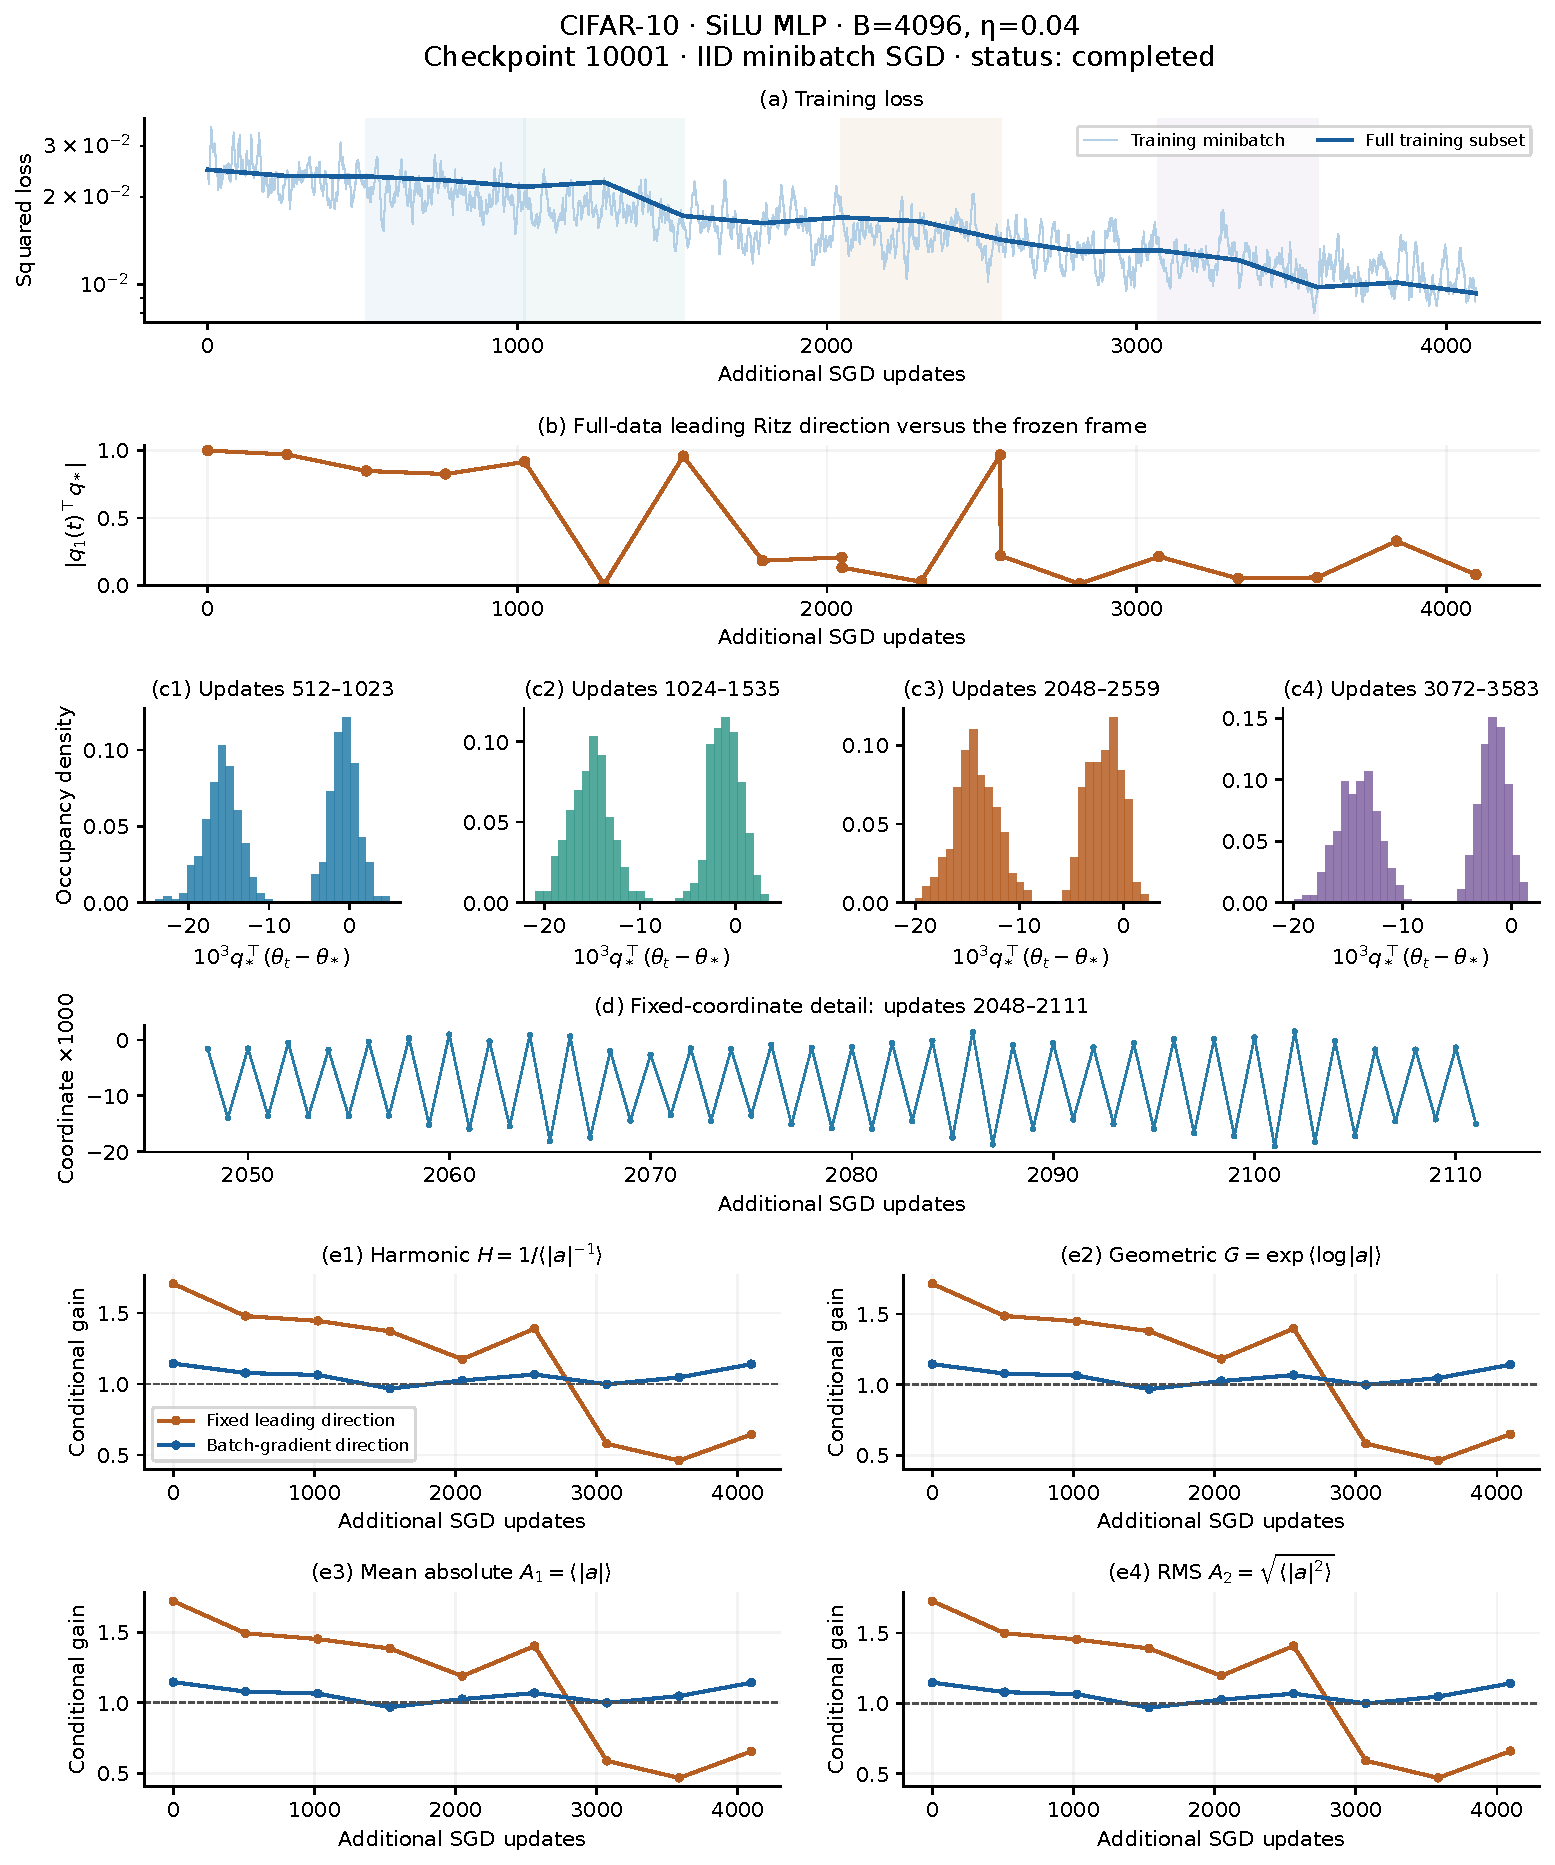
\includegraphics[width=\linewidth,height=0.78\textheight,keepaspectratio]{img/current_results/fig01_mlp_loss_alignment_bimodality.pdf}
\caption{The center and plotting direction are fixed at the parent checkpoint. All runs use IID subsets, original parent learning rate, and the full 8192-example training subset. Curvature matrices in the alignment panel use that same subset. Histograms use four declared 512-update intervals and 30 bins without selecting intervals by modality. The short trace uses updates2048--2111. Gain ladders use fresh minibatches at each plotted state: fixed-axis compression versus batch-gradient compression, each summarized by H,G,A1,A2. No propagated-tangent panel and no static ladder panels are included. Sparse even-update conditional probes do not average over oscillation phases; they do not establish stationarity or a full-network Lyapunov exponent. Alignment is measured, not assumed, and Ritz extremality is not certified. The original anchor uses128 fresh draws at zero and24 at subsequent even states512k.}
\label{fig:current-fig01-mlp-loss-alignment-bimodality}
\end{figure}\clearpage

\begin{figure}[p]\centering
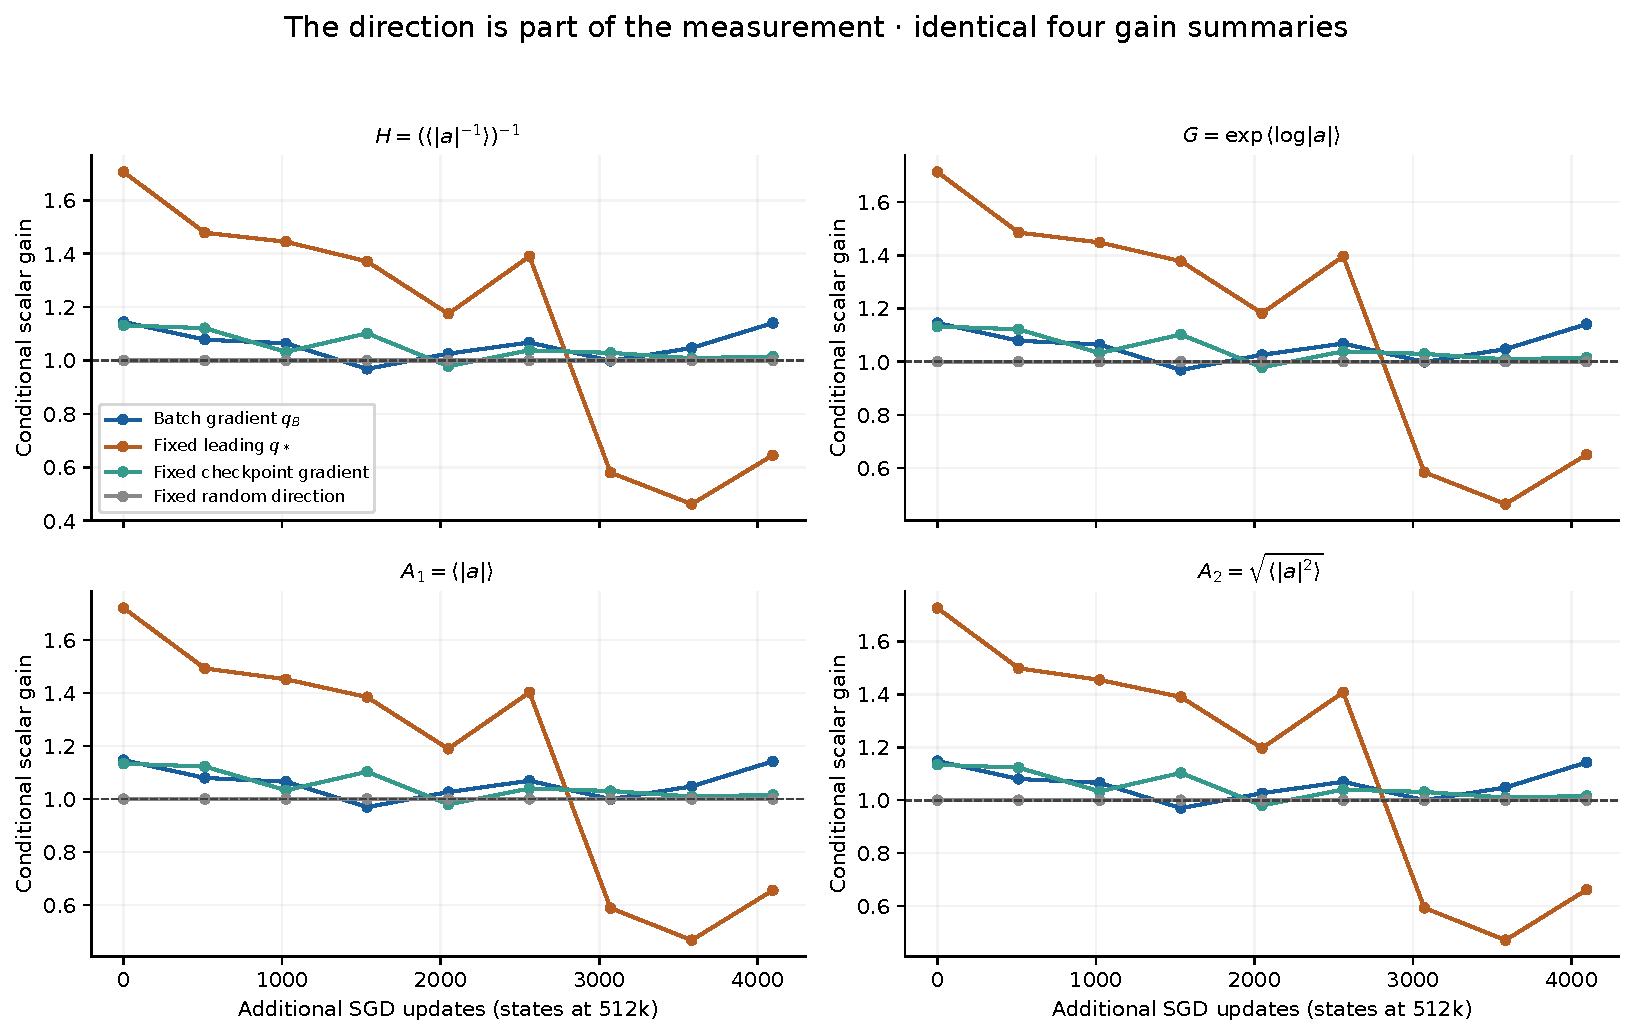
\includegraphics[width=\linewidth,height=0.78\textheight,keepaspectratio]{img/current_results/fig02_direction_resolved_ladder.pdf}
\caption{Fresh conditional minibatch probes at each displayed fixed state, using the same draws across directions. There are 128 draws at update zero and 24 at other displayed states. Only states at multiples of 512 are displayed here; the adjacent phase appears in Figure 3. The batch-gradient direction changes with the sampled batch. All other directions are checkpoint-fixed. Geometric gain G=exp(Lambda) shares the unit reference with H, A1 and A2. Finite H does not establish a finite population inverse moment.}
\label{fig:current-fig02-direction-resolved-ladder}
\end{figure}\clearpage

\begin{figure}[p]\centering
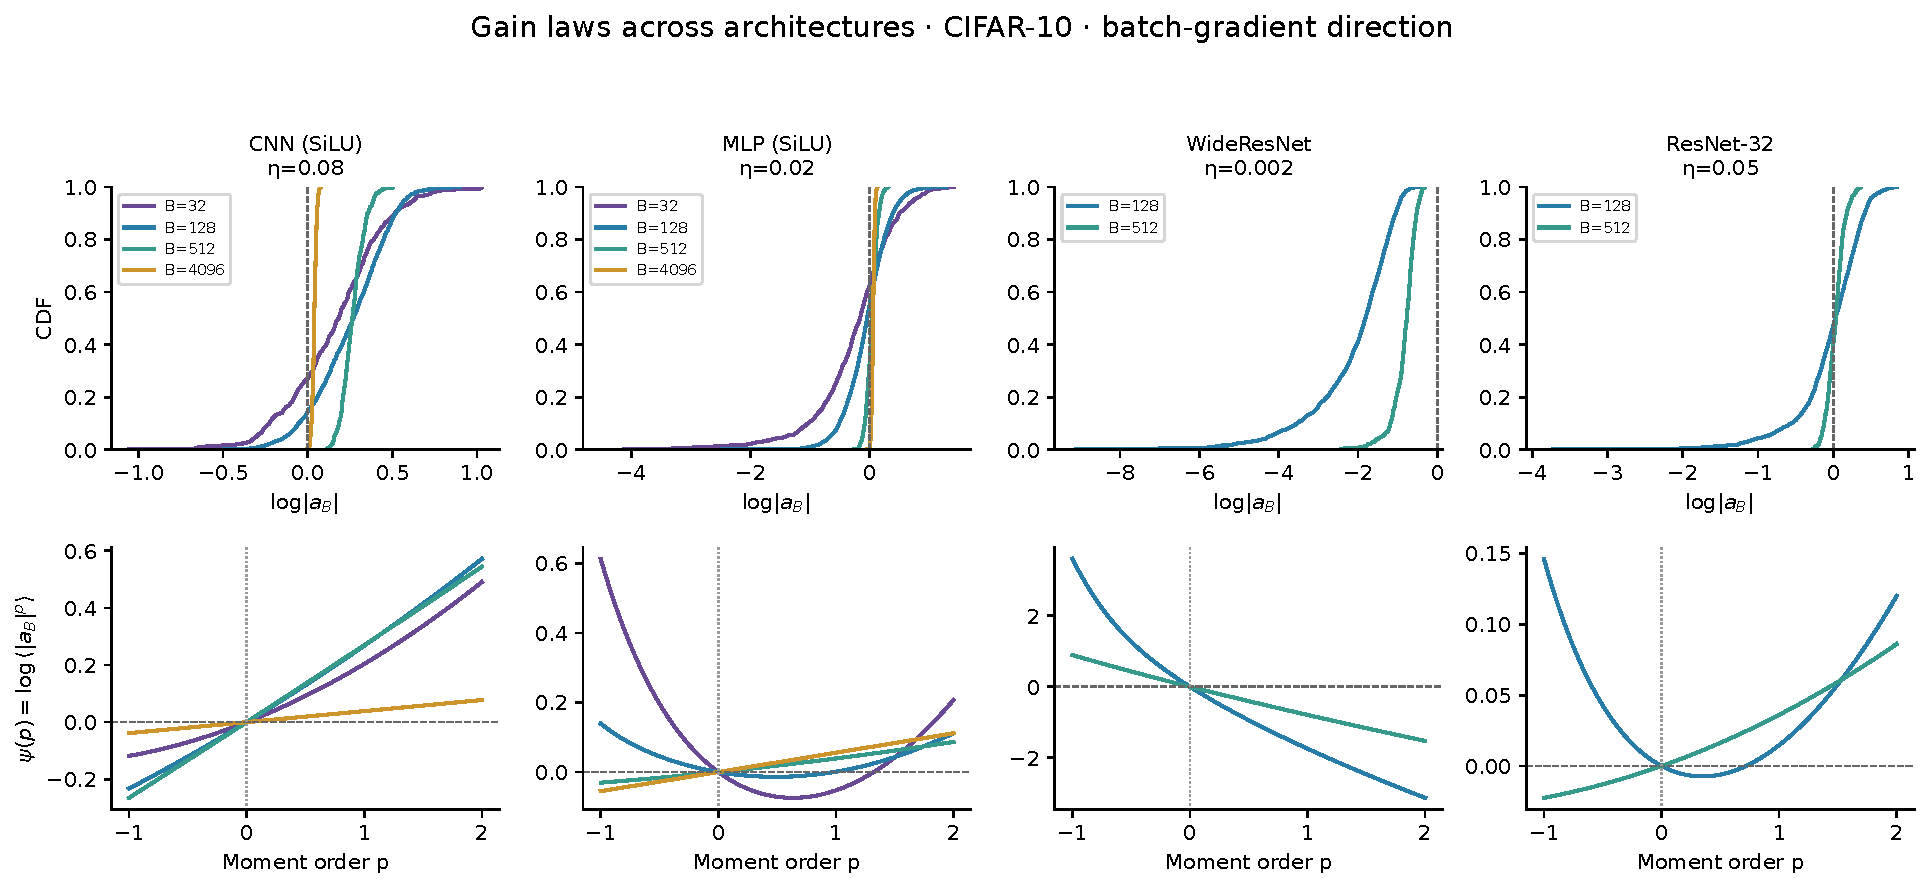
\includegraphics[width=\linewidth,height=0.78\textheight,keepaspectratio]{img/current_results/fig04_cross_architecture_gain_laws.pdf}
\caption{Batch-gradient scalar gains at update 20000 and matched training/probe batch size. Curves average within-run CDFs or log moments equally across available runs; this is not the log moment of pooled gains. No separate seed panels. Architecture-specific step sizes are labeled; this is not a controlled comparison changing architecture alone. Only measured final-checkpoint cases are shown; the full grids retain earlier/pre-escape observations. Positive and negative moments summarize gain distributions, not parameter-coordinate histograms.}
\label{fig:current-fig04-cross-architecture-gain-laws}
\end{figure}\clearpage

\begin{figure}[p]\centering
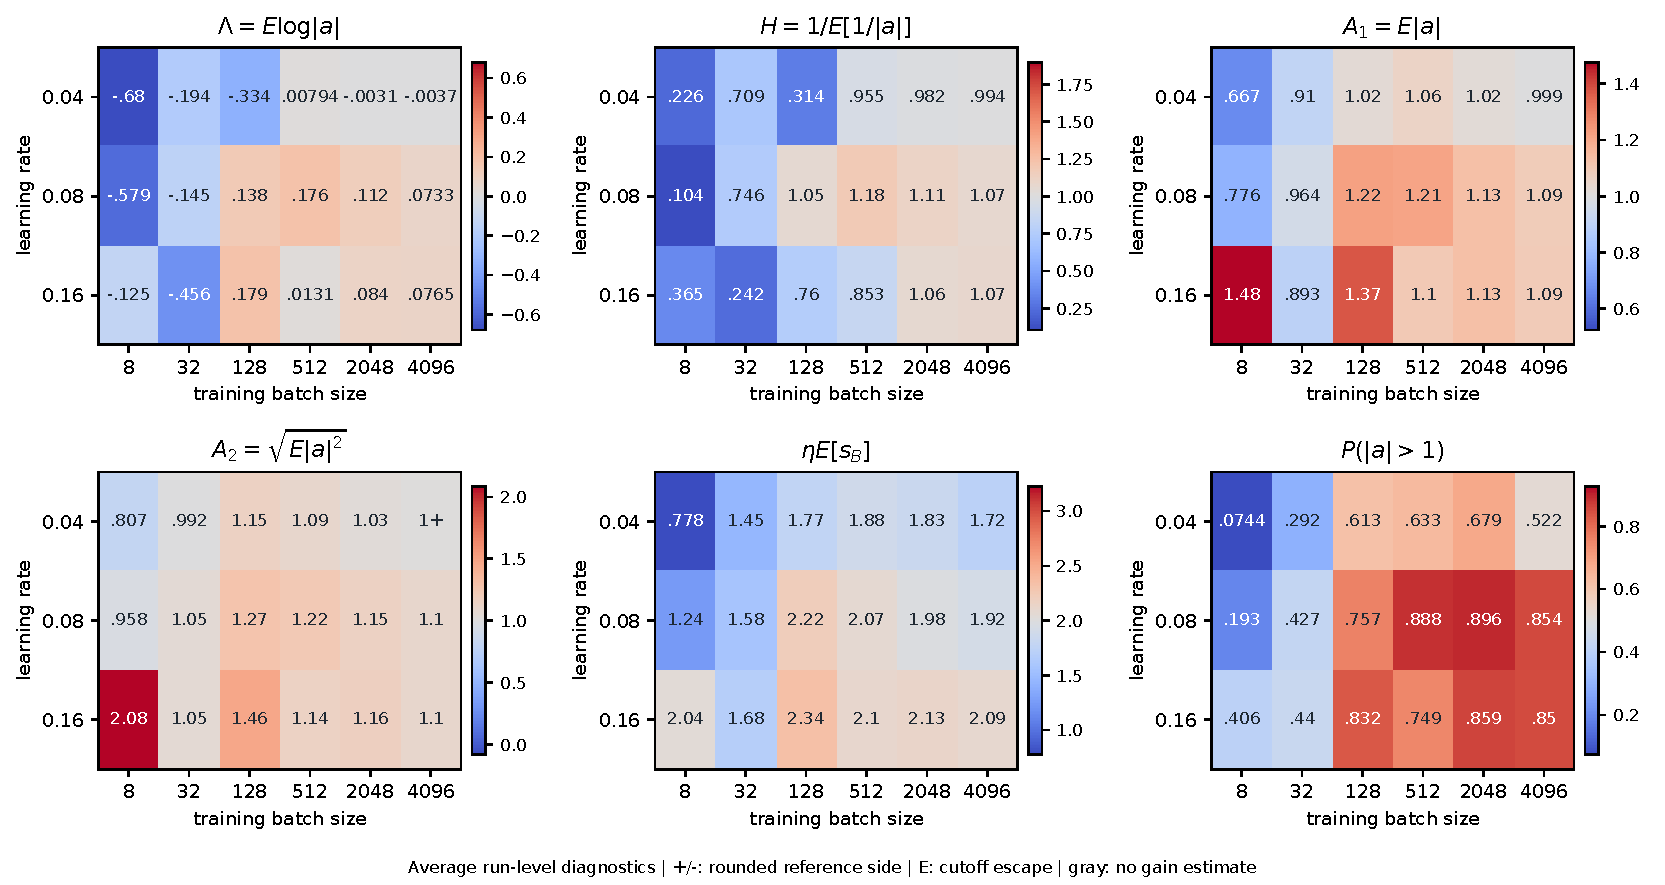
\includegraphics[width=\linewidth,height=0.78\textheight,keepaspectratio]{img/current_results/cnn_silu_grid_eta_batch.pdf}
\caption{\textbf{CNN with SiLU | stability grid over batch size and step size.} Axes are actual training learning rate and batch size. The six panels show Lambda, H, A1, A2, eta E[s\_B], and the fraction of expanding gains. Each cell averages run-level statistics from the final three available checkpoints; time windows can differ across settings and runs. Color centers are 0, 1, 1, 1, 2, and 0.5. Curvature and expansion-fraction centers are references, not full-network stability tests. A trailing +/- preserves the side of a reference after rounding. Gray means no gain estimate; E marks a recorded escape, including pre-escape estimates. Finite H does not establish population inverse-moment finiteness.}
\label{fig:current-cnn-silu-grid-eta-batch}
\end{figure}\clearpage

\begin{figure}[p]\centering
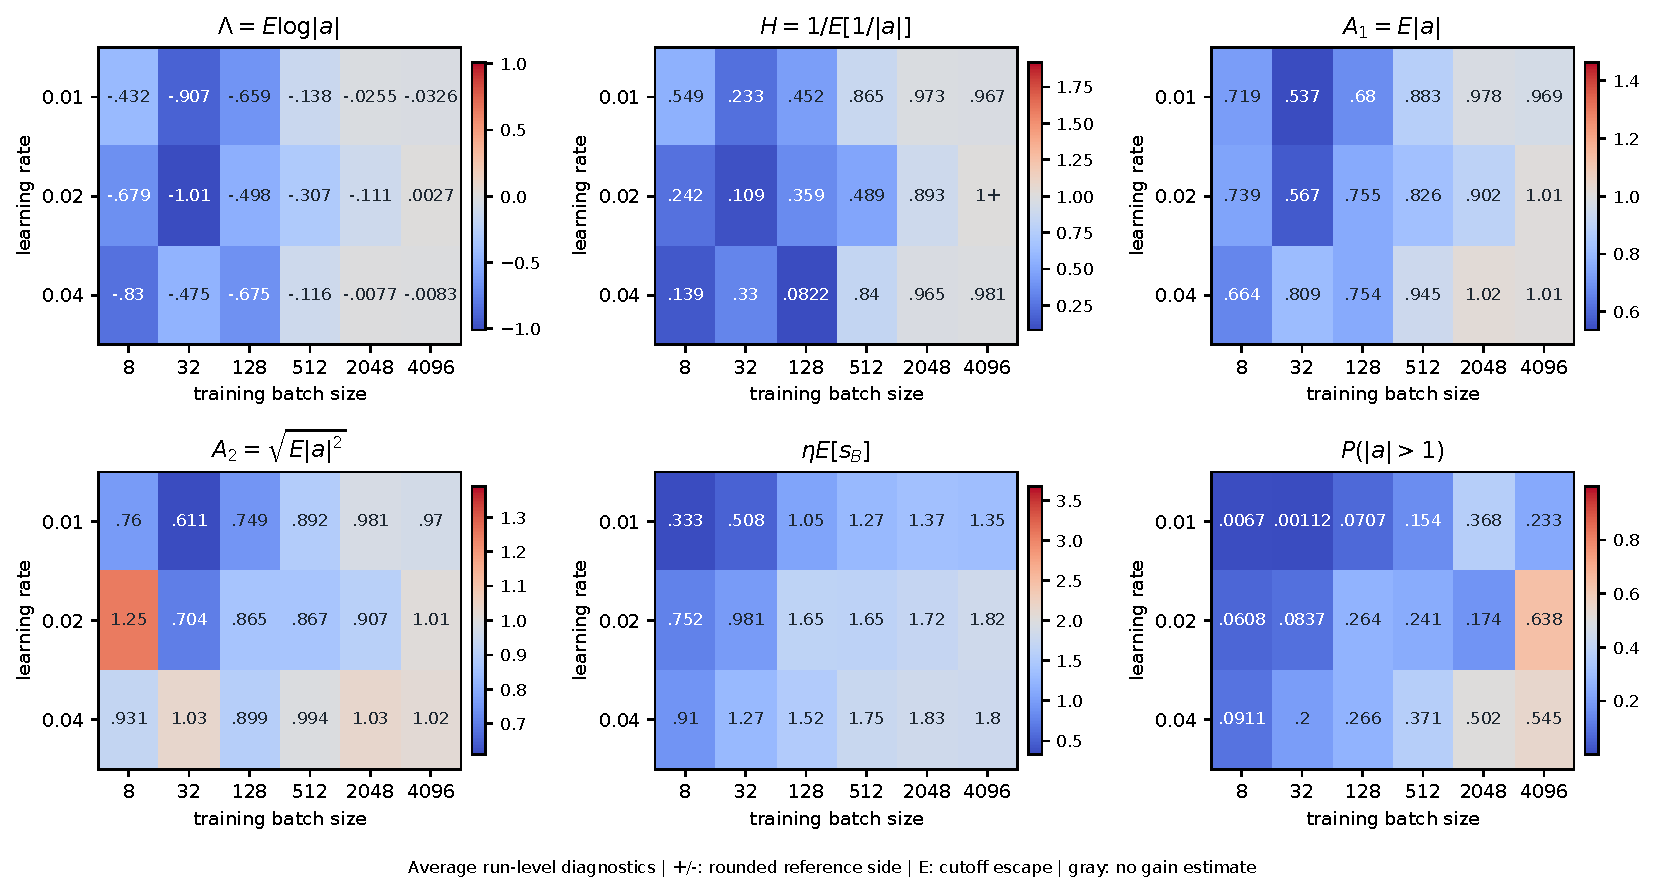
\includegraphics[width=\linewidth,height=0.78\textheight,keepaspectratio]{img/current_results/mlp_silu_grid_eta_batch.pdf}
\caption{\textbf{MLP, 2 x 512 (SiLU) | stability grid over batch size and step size.} Axes are actual training learning rate and batch size. The six panels show Lambda, H, A1, A2, eta E[s\_B], and the fraction of expanding gains. Each cell averages run-level statistics from the final three available checkpoints; time windows can differ across settings and runs. Color centers are 0, 1, 1, 1, 2, and 0.5. Curvature and expansion-fraction centers are references, not full-network stability tests. A trailing +/- preserves the side of a reference after rounding. Gray means no gain estimate; E marks a recorded escape, including pre-escape estimates. Finite H does not establish population inverse-moment finiteness.}
\label{fig:current-mlp-silu-grid-eta-batch}
\end{figure}\clearpage

\begin{figure}[p]\centering
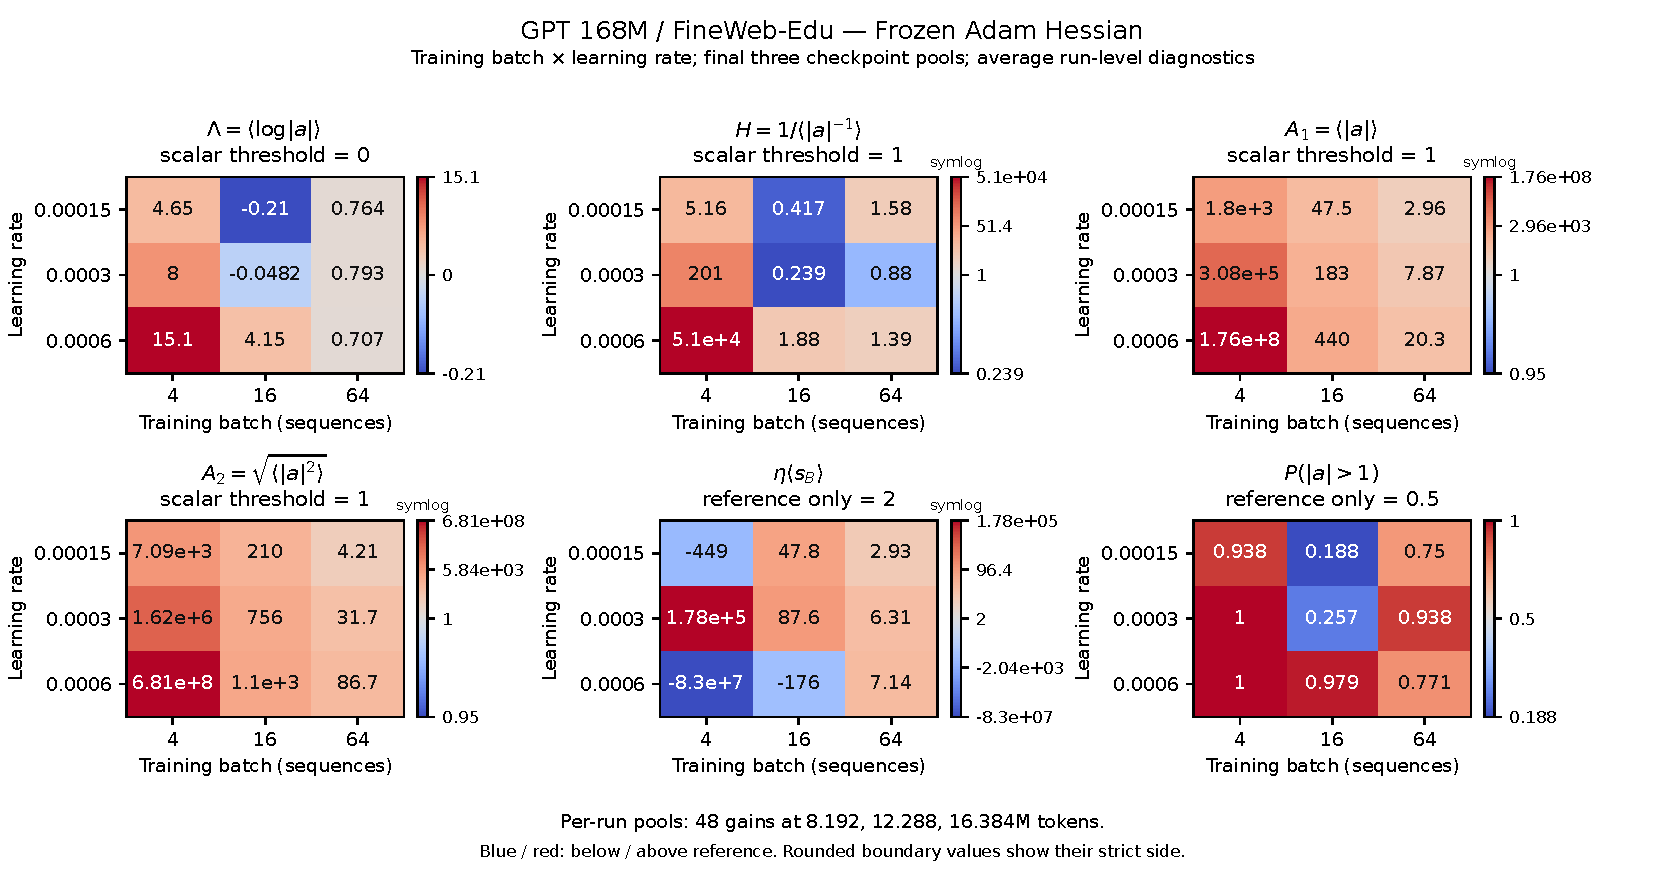
\includegraphics[width=\linewidth,height=0.78\textheight,keepaspectratio]{img/current_results/gpt_grid03_frozen_adam_hessian.pdf}
\caption{\textbf{GPT / FineWeb-Edu: batch--step-size grid, frozen adam hessian.} Frozen Adam Hessian; all nine batch-rate cells retained. Values average run-level statistics from final-three-checkpoint pools at 8.192, 12.288 and 16.384 million tokens. Blue/red means below/above the panel reference. Pools contain 48 Hessian or 24 GGN gains per run. Annotations use three significant figures, with strict inequalities when rounded to a threshold. Symlog colorbars retain extreme values; ticks use original units. Eta E[s\_B]=2 and P(|a|>1)=0.5 are references, not stability certificates. Small inverse-moment samples do not establish population finiteness or stationarity. Parents use Adam: raw metrics are scalar SGD counterfactuals; frozen metrics exclude momentum and preconditioner evolution. Neither is a full-Adam Jacobian.}
\label{fig:current-gpt-grid03-frozen-adam-hessian}
\end{figure}\clearpage

\section*{Architecture and dataset atlas}

\begin{figure}[p]\centering
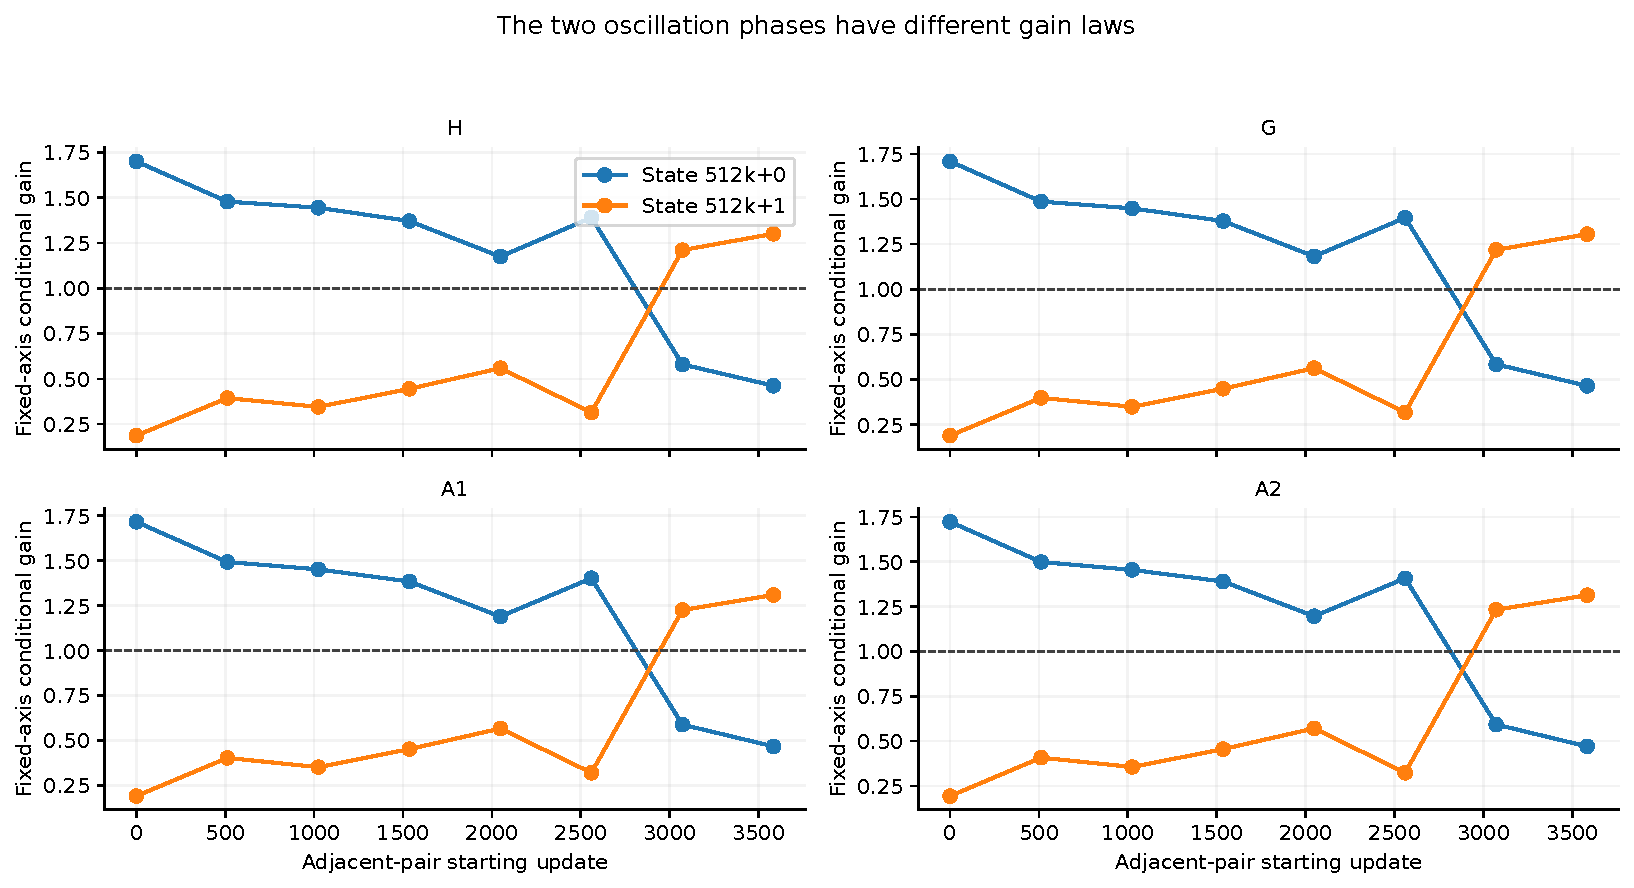
\includegraphics[width=\linewidth,height=0.78\textheight,keepaspectratio]{img/current_results/fig03_paired_phase_ladder.pdf}
\caption{Fixed leading-axis scalar gains: 24 identical fresh minibatches reused across the two states of each adjacent pair. All four measures are computed separately by phase. These are conditional one-step compression statistics, not the two-step product exponent.}
\label{fig:current-fig03-paired-phase-ladder}
\end{figure}\clearpage

\begin{figure}[p]\centering
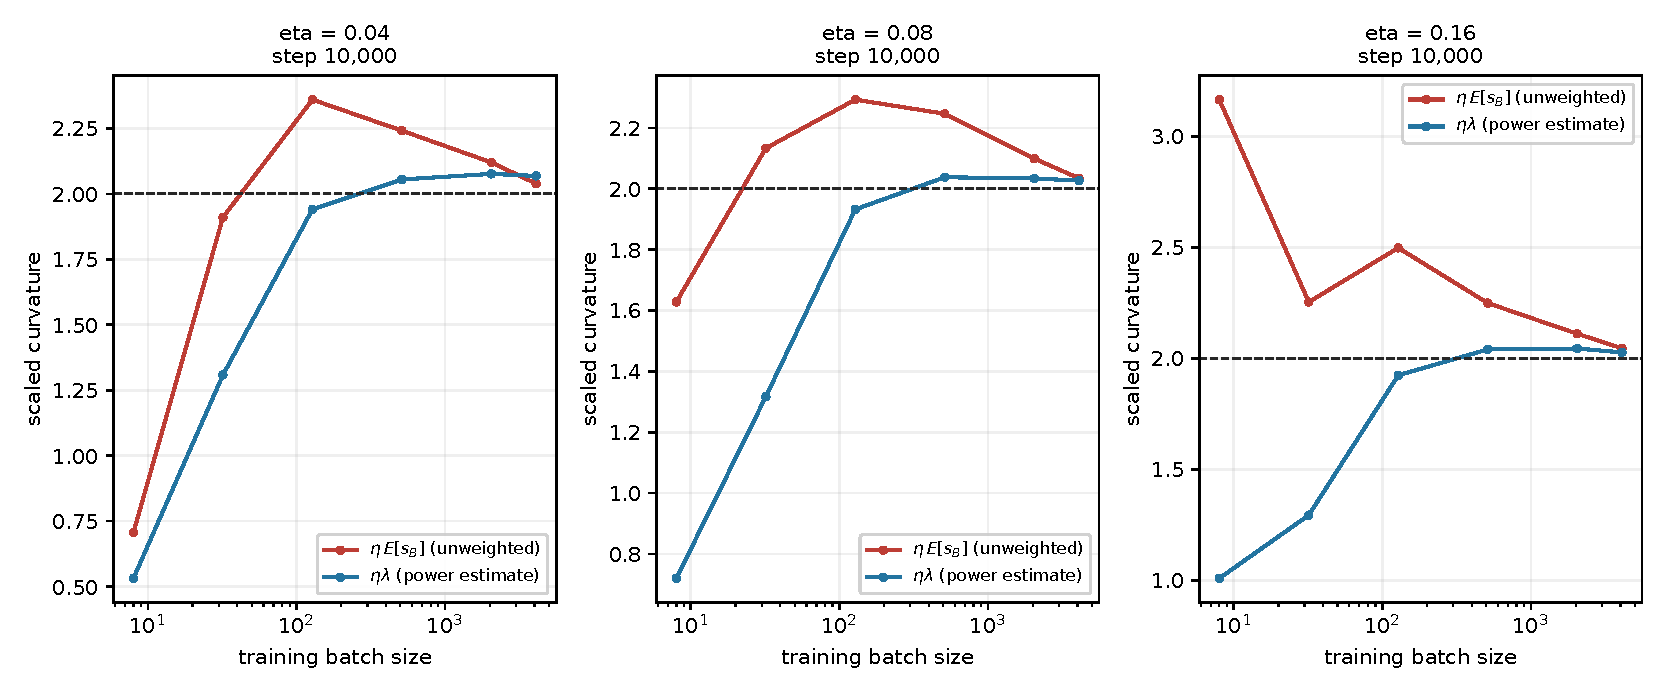
\includegraphics[width=\linewidth,height=0.78\textheight,keepaspectratio]{img/current_results/cnn_silu_01_curvature.pdf}
\caption{\textbf{CNN with SiLU | curvature thresholds.} eta=0.04: step 10,000; eta=0.08: step 10,000; eta=0.16: step 10,000. Curves show average run-level measurements. The Hessian curve is a finite power-iteration estimate; it is not a certified largest eigenvalue. Actual saved learning rates are used. A red cross retains a pre-escape checkpoint.}
\label{fig:current-cnn-silu-01-curvature}
\end{figure}\clearpage

\begin{figure}[p]\centering
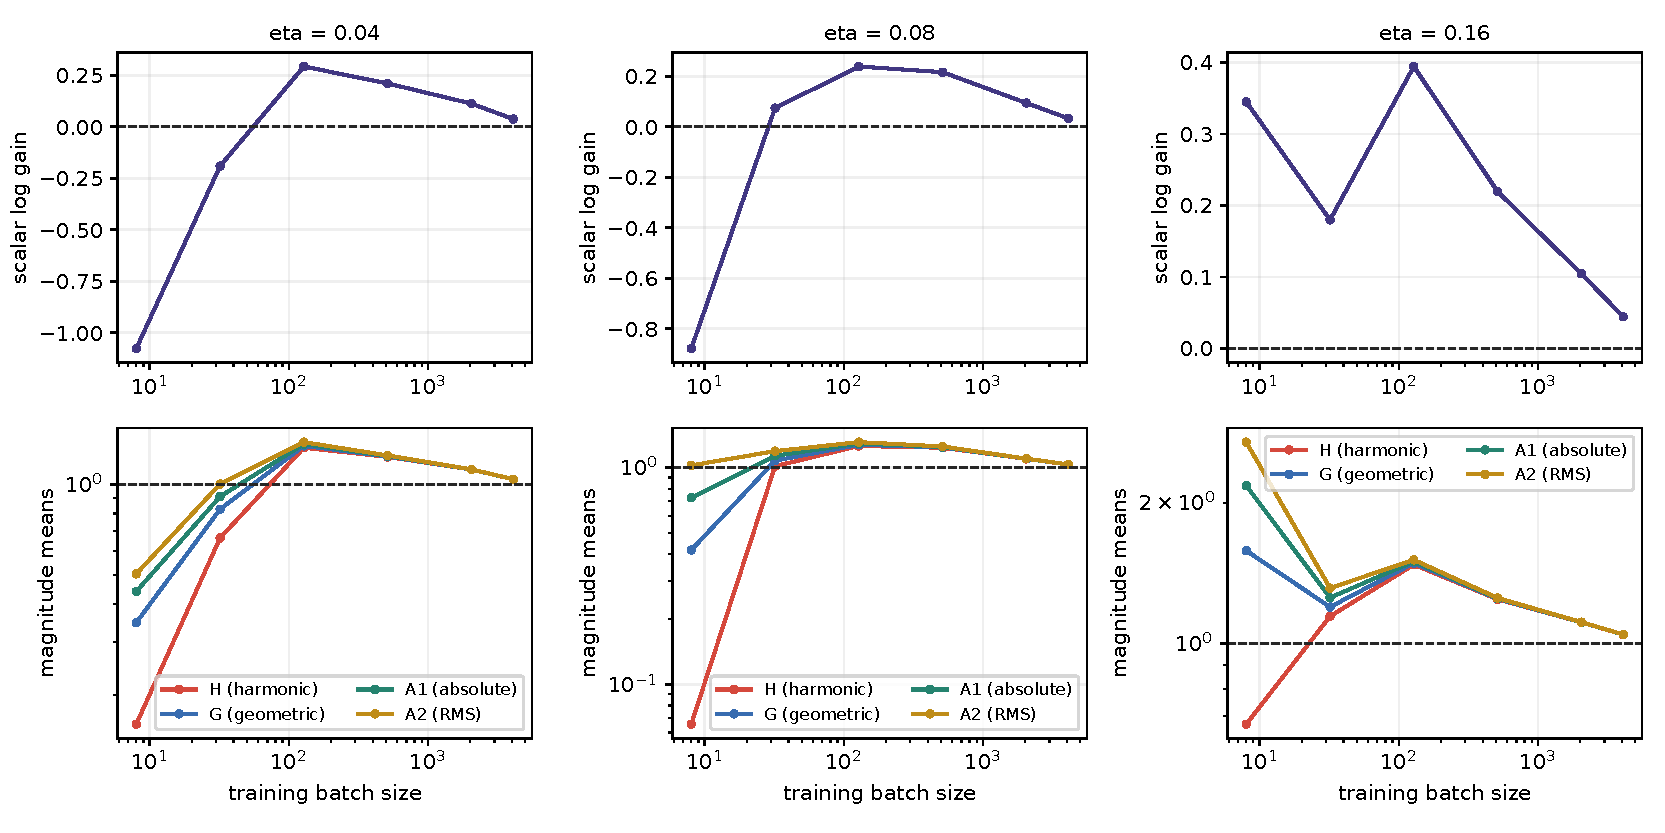
\includegraphics[width=\linewidth,height=0.78\textheight,keepaspectratio]{img/current_results/cnn_silu_02_moments.pdf}
\caption{\textbf{CNN with SiLU | the moment ladder.} eta=0.04: step 10,000; eta=0.08: step 10,000; eta=0.16: step 10,000. Curves show average run-level measurements. H=1/E[1/|a|], G=exp(Lambda), A1=E|a|, A2=sqrt(E|a|\textasciicircum{}2). The lower panel uses a logarithmic scale. A mean of run-level H estimates is not H of a pooled distribution; finite estimates do not prove inverse-moment existence.}
\label{fig:current-cnn-silu-02-moments}
\end{figure}\clearpage

\begin{figure}[p]\centering
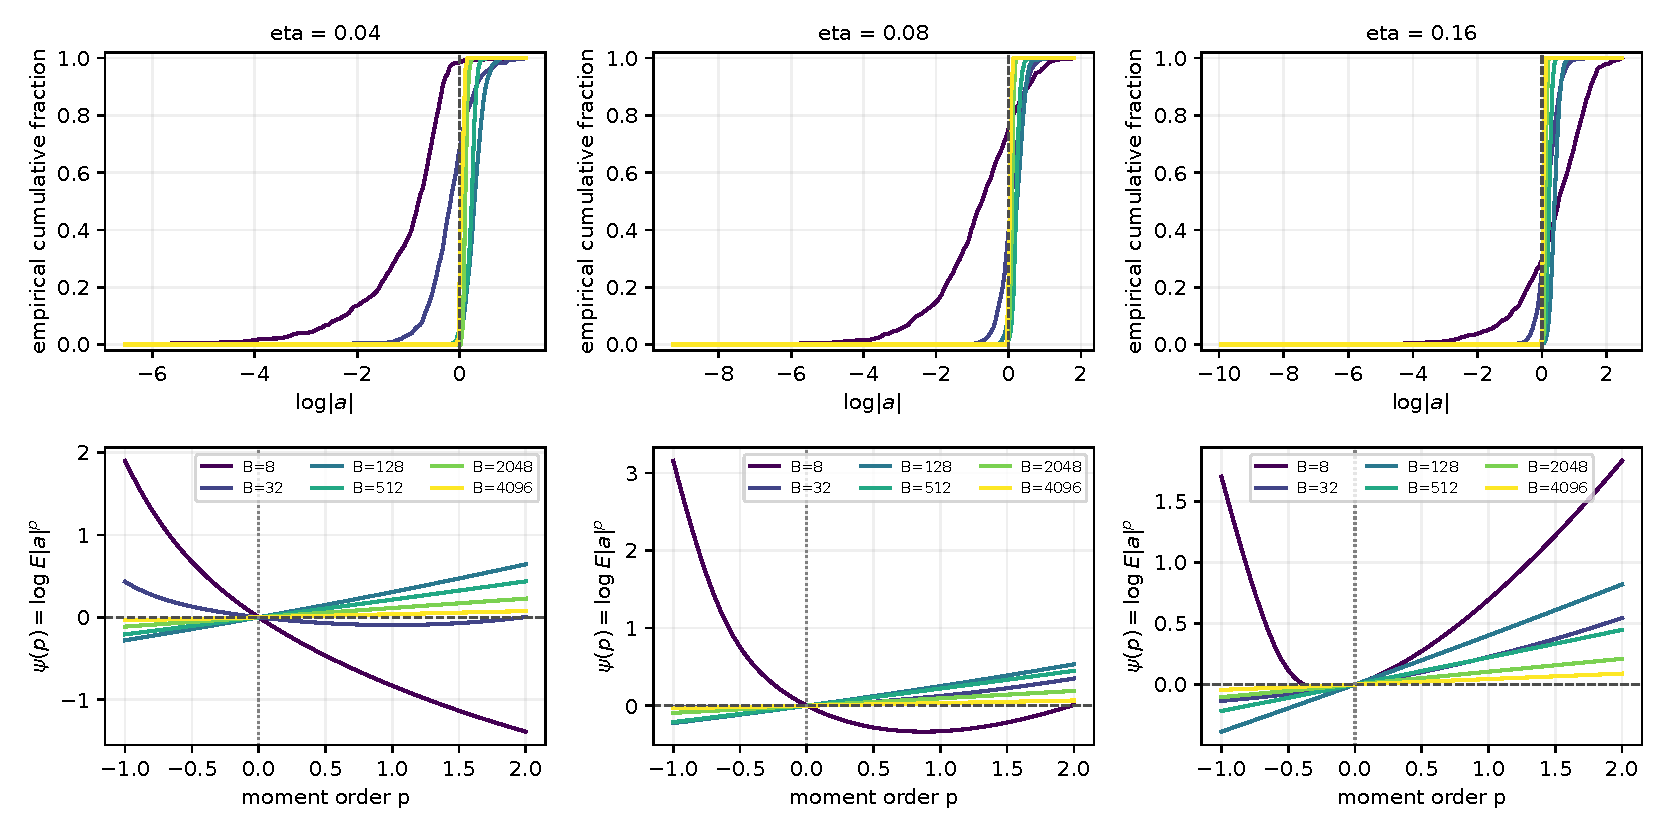
\includegraphics[width=\linewidth,height=0.78\textheight,keepaspectratio]{img/current_results/cnn_silu_03_gain_law.pdf}
\caption{\textbf{CNN with SiLU | gain distributions and moment pressure.} eta=0.04: step 10,000; eta=0.08: step 10,000; eta=0.16: step 10,000. Curves show average run-level measurements. CDFs and log moments are computed within each run, then averaged equally. These are distributions of a conditional scalar multiplier, not distributions of a fixed parameter coordinate. Values near a=0 dominate inverse moments; p=0 is exactly zero by definition.}
\label{fig:current-cnn-silu-03-gain-law}
\end{figure}\clearpage

\begin{figure}[p]\centering
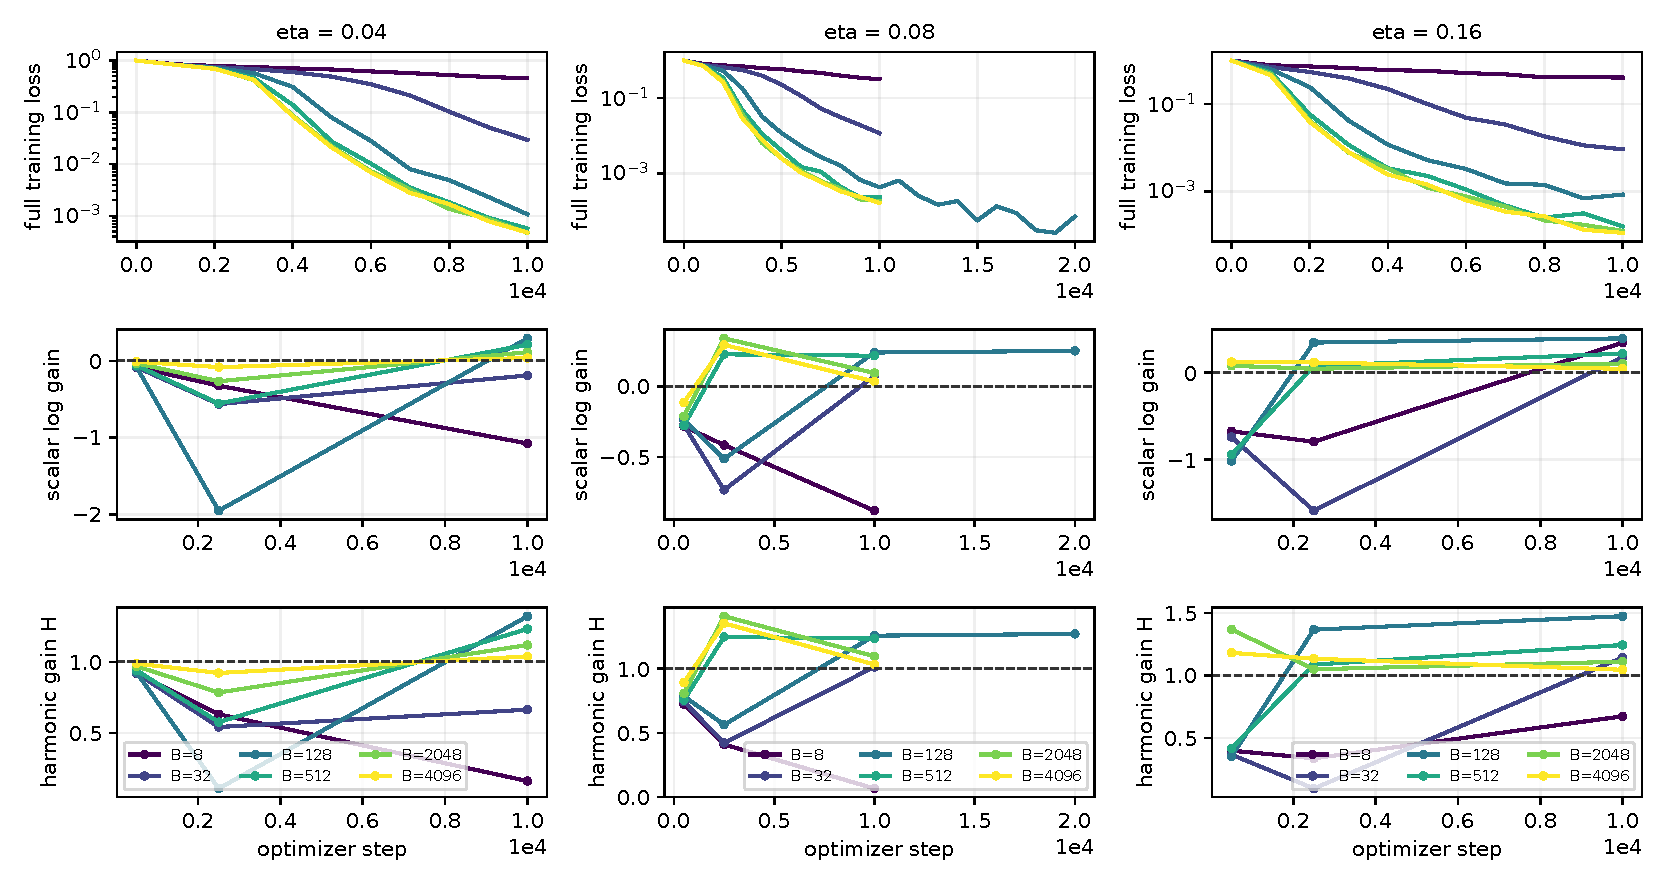
\includegraphics[width=\linewidth,height=0.78\textheight,keepaspectratio]{img/current_results/cnn_silu_04_dynamics.pdf}
\caption{\textbf{CNN with SiLU | training and conditional gain dynamics.} Each batch curve averages run-level measurements at shared checkpoints and stops at the last common measurement. Loss and gain panels use their own recorded sampling grids. Finite training prefixes and decreasing loss do not establish a stationary distribution.}
\label{fig:current-cnn-silu-04-dynamics}
\end{figure}\clearpage

\begin{figure}[p]\centering
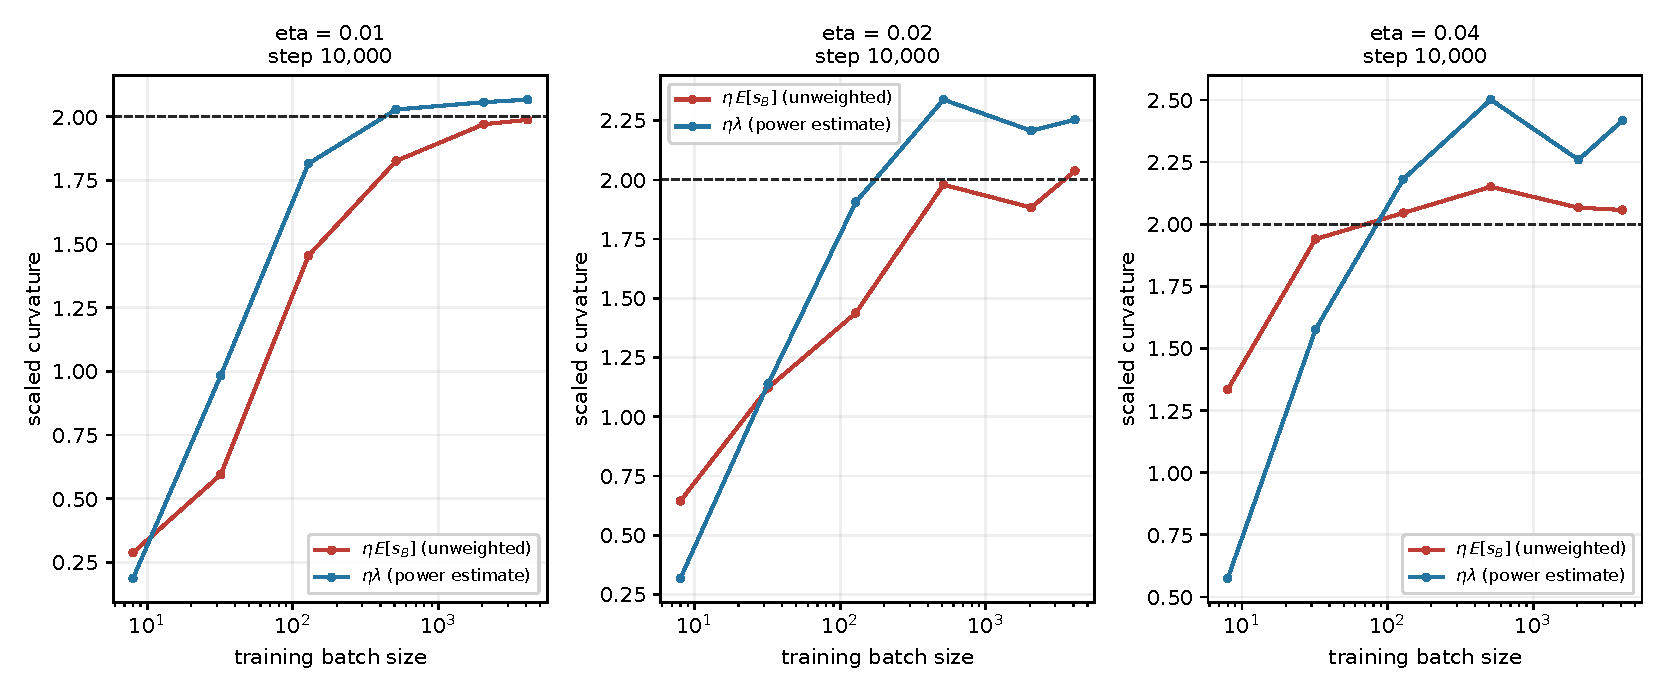
\includegraphics[width=\linewidth,height=0.78\textheight,keepaspectratio]{img/current_results/mlp_silu_01_curvature.pdf}
\caption{\textbf{MLP, 2 x 512 (SiLU) | curvature thresholds.} eta=0.01: step 10,000; eta=0.02: step 10,000; eta=0.04: step 10,000. Curves show average run-level measurements. The Hessian curve is a finite power-iteration estimate; it is not a certified largest eigenvalue. Actual saved learning rates are used. A red cross retains a pre-escape checkpoint.}
\label{fig:current-mlp-silu-01-curvature}
\end{figure}\clearpage

\begin{figure}[p]\centering
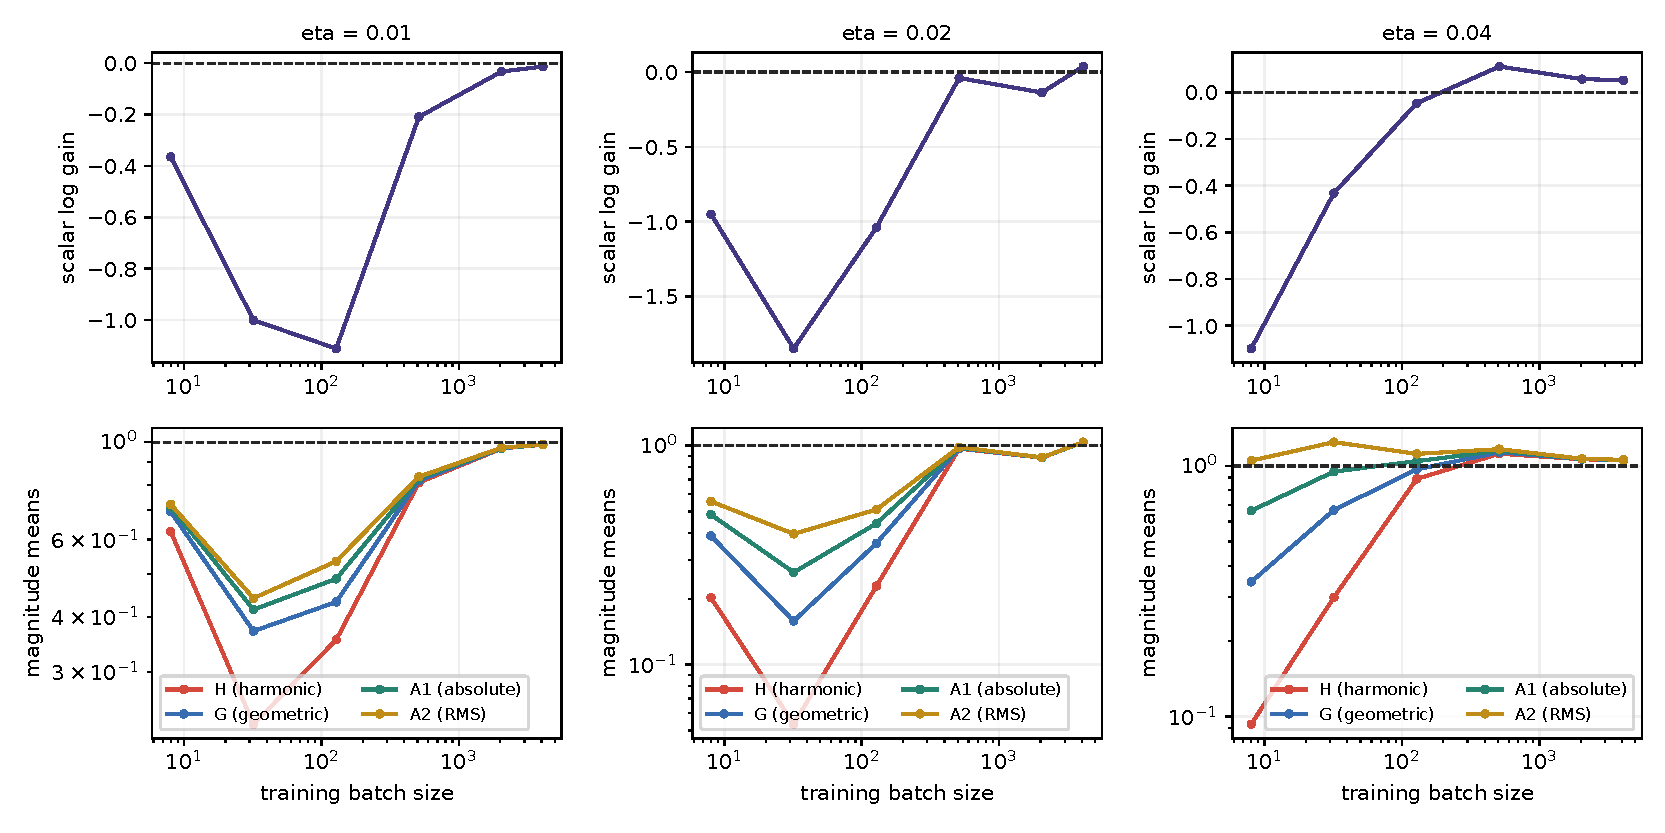
\includegraphics[width=\linewidth,height=0.78\textheight,keepaspectratio]{img/current_results/mlp_silu_02_moments.pdf}
\caption{\textbf{MLP, 2 x 512 (SiLU) | the moment ladder.} eta=0.01: step 10,000; eta=0.02: step 10,000; eta=0.04: step 10,000. Curves show average run-level measurements. H=1/E[1/|a|], G=exp(Lambda), A1=E|a|, A2=sqrt(E|a|\textasciicircum{}2). The lower panel uses a logarithmic scale. A mean of run-level H estimates is not H of a pooled distribution; finite estimates do not prove inverse-moment existence.}
\label{fig:current-mlp-silu-02-moments}
\end{figure}\clearpage

\begin{figure}[p]\centering
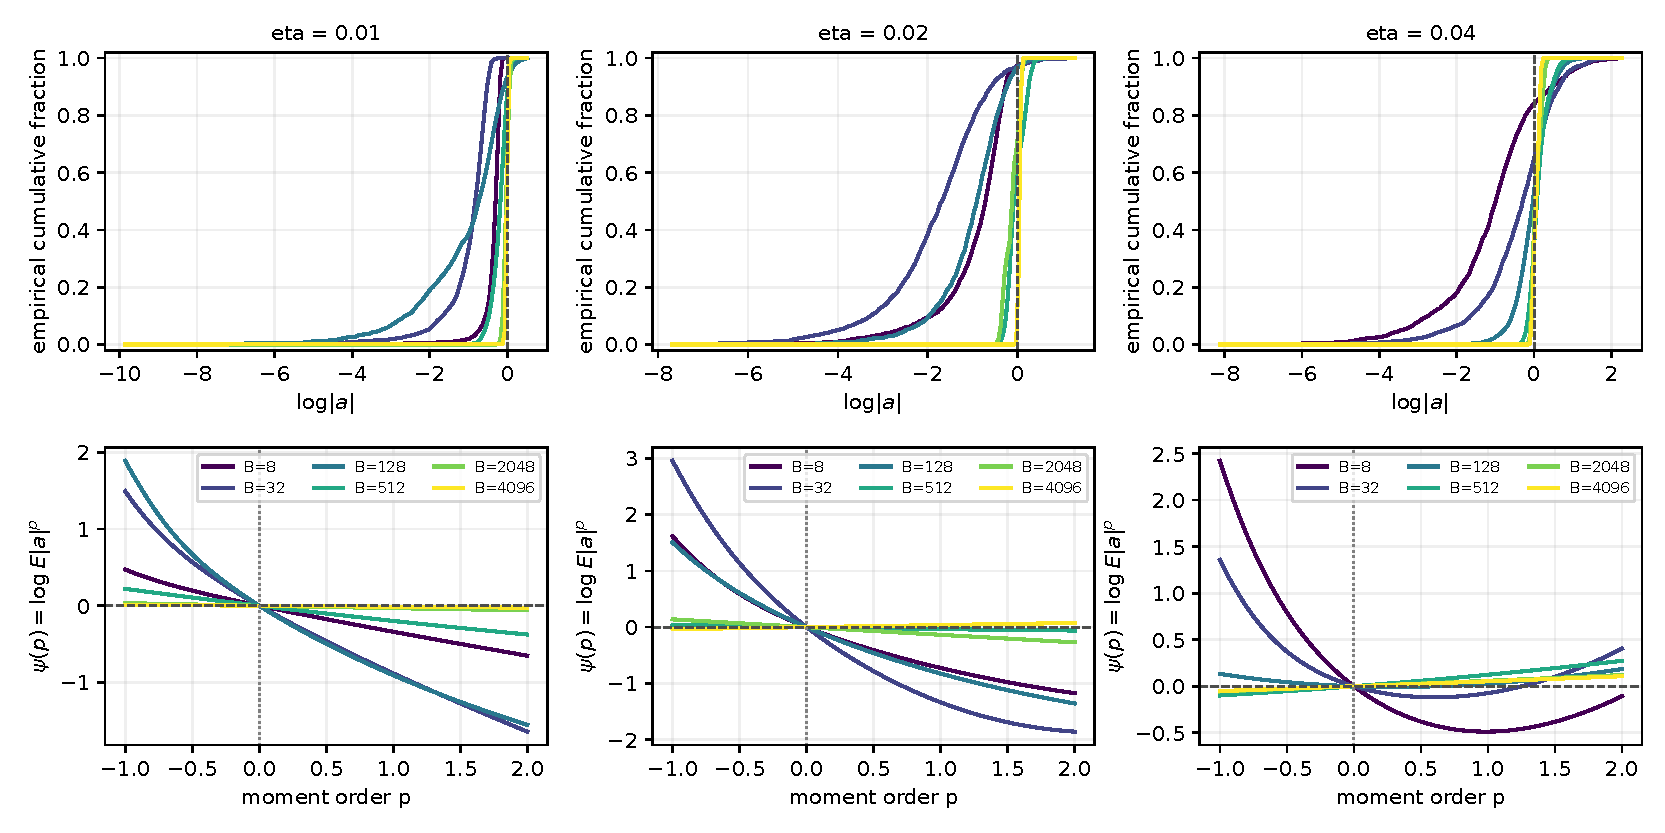
\includegraphics[width=\linewidth,height=0.78\textheight,keepaspectratio]{img/current_results/mlp_silu_03_gain_law.pdf}
\caption{\textbf{MLP, 2 x 512 (SiLU) | gain distributions and moment pressure.} eta=0.01: step 10,000; eta=0.02: step 10,000; eta=0.04: step 10,000. Curves show average run-level measurements. CDFs and log moments are computed within each run, then averaged equally. These are distributions of a conditional scalar multiplier, not distributions of a fixed parameter coordinate. Values near a=0 dominate inverse moments; p=0 is exactly zero by definition.}
\label{fig:current-mlp-silu-03-gain-law}
\end{figure}\clearpage

\begin{figure}[p]\centering
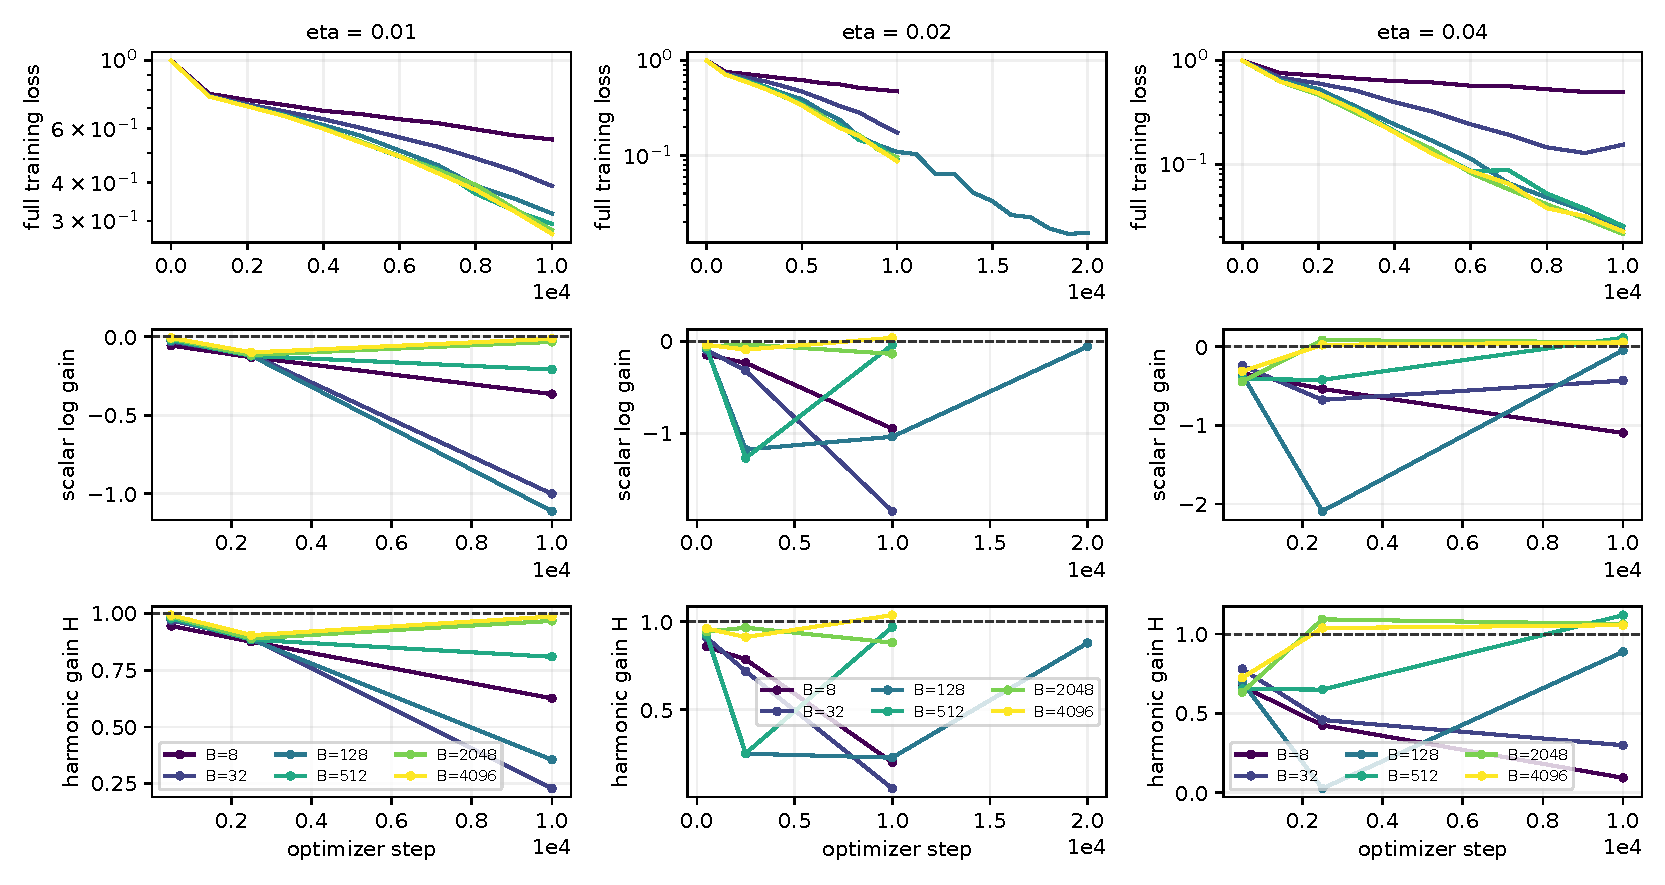
\includegraphics[width=\linewidth,height=0.78\textheight,keepaspectratio]{img/current_results/mlp_silu_04_dynamics.pdf}
\caption{\textbf{MLP, 2 x 512 (SiLU) | training and conditional gain dynamics.} Each batch curve averages run-level measurements at shared checkpoints and stops at the last common measurement. Loss and gain panels use their own recorded sampling grids. Finite training prefixes and decreasing loss do not establish a stationary distribution.}
\label{fig:current-mlp-silu-04-dynamics}
\end{figure}\clearpage

\begin{figure}[p]\centering
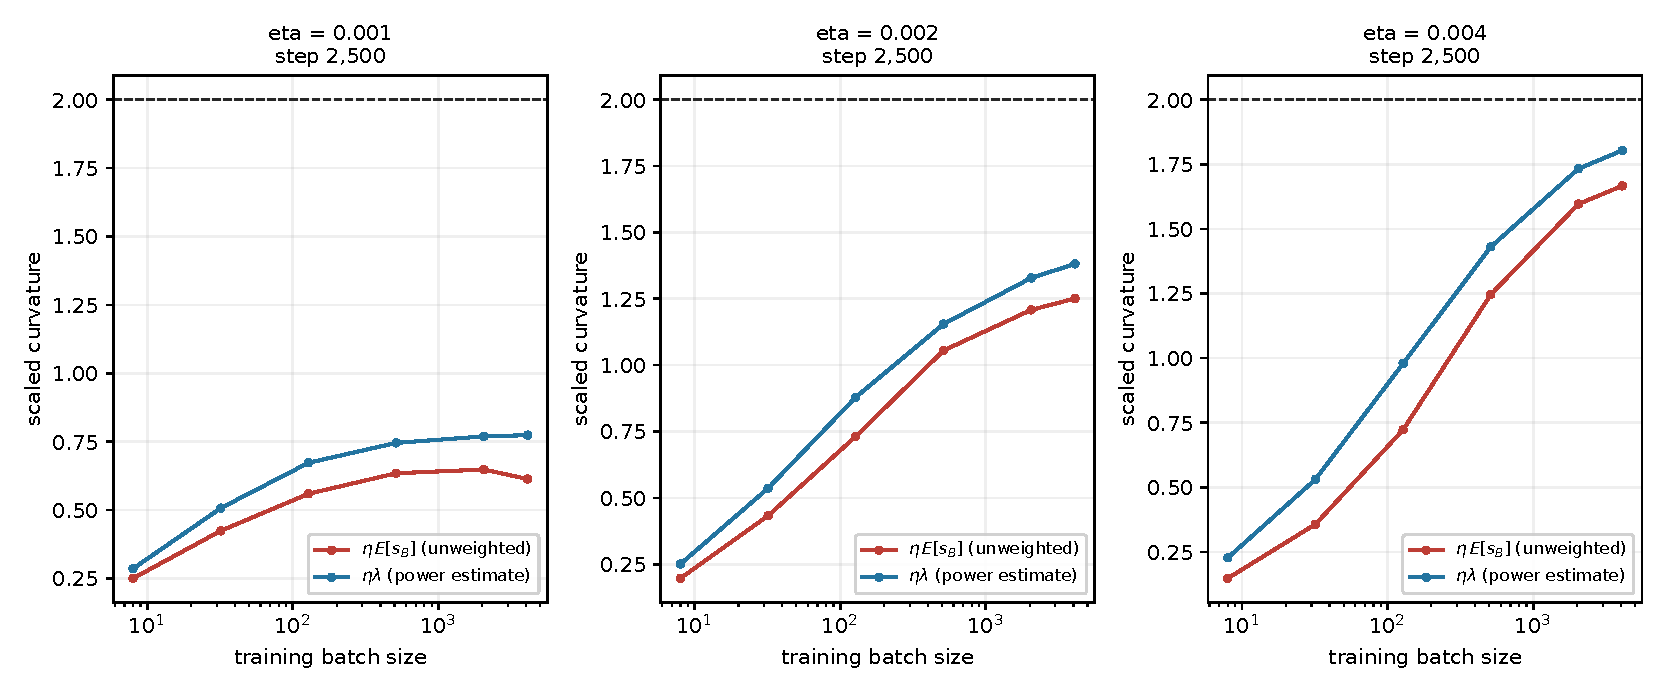
\includegraphics[width=\linewidth,height=0.78\textheight,keepaspectratio]{img/current_results/wrn_no_bn_01_curvature.pdf}
\caption{\textbf{WideResNet-10-2, native Fixup | curvature thresholds.} eta=0.001: step 2,500; eta=0.002: step 2,500; eta=0.004: step 2,500. Curves show average run-level measurements. The Hessian curve is a finite power-iteration estimate; it is not a certified largest eigenvalue. Actual saved learning rates are used. A red cross retains a pre-escape checkpoint.}
\label{fig:current-wrn-no-bn-01-curvature}
\end{figure}\clearpage

\begin{figure}[p]\centering
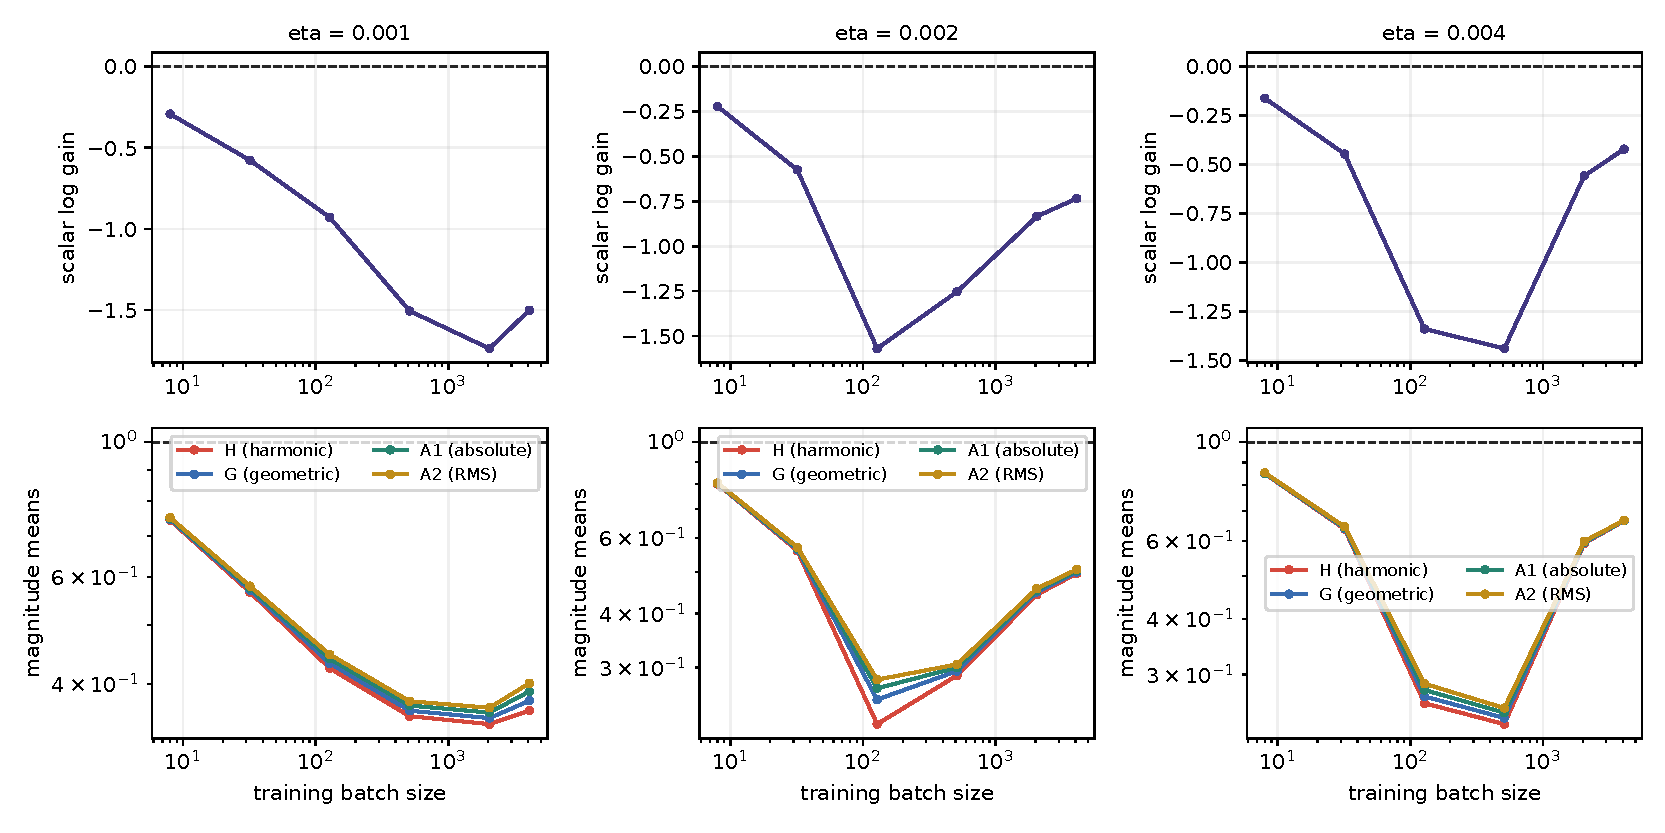
\includegraphics[width=\linewidth,height=0.78\textheight,keepaspectratio]{img/current_results/wrn_no_bn_02_moments.pdf}
\caption{\textbf{WideResNet-10-2, native Fixup | the moment ladder.} eta=0.001: step 2,500; eta=0.002: step 2,500; eta=0.004: step 2,500. Curves show average run-level measurements. H=1/E[1/|a|], G=exp(Lambda), A1=E|a|, A2=sqrt(E|a|\textasciicircum{}2). The lower panel uses a logarithmic scale. A mean of run-level H estimates is not H of a pooled distribution; finite estimates do not prove inverse-moment existence.}
\label{fig:current-wrn-no-bn-02-moments}
\end{figure}\clearpage

\begin{figure}[p]\centering
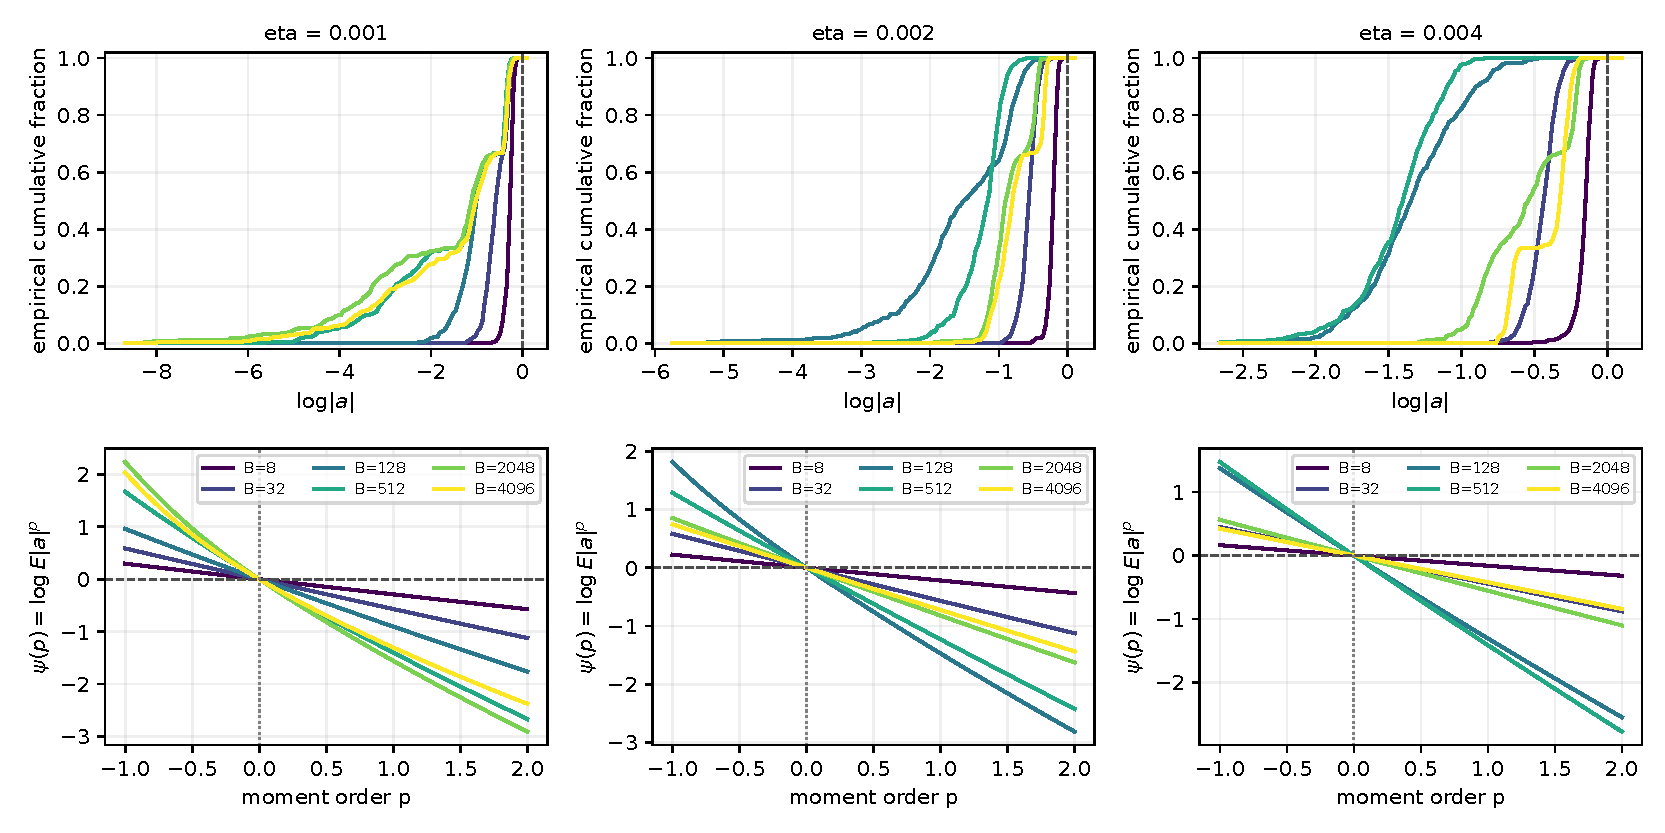
\includegraphics[width=\linewidth,height=0.78\textheight,keepaspectratio]{img/current_results/wrn_no_bn_03_gain_law.pdf}
\caption{\textbf{WideResNet-10-2, native Fixup | gain distributions and moment pressure.} eta=0.001: step 2,500; eta=0.002: step 2,500; eta=0.004: step 2,500. Curves show average run-level measurements. CDFs and log moments are computed within each run, then averaged equally. These are distributions of a conditional scalar multiplier, not distributions of a fixed parameter coordinate. Values near a=0 dominate inverse moments; p=0 is exactly zero by definition.}
\label{fig:current-wrn-no-bn-03-gain-law}
\end{figure}\clearpage

\begin{figure}[p]\centering
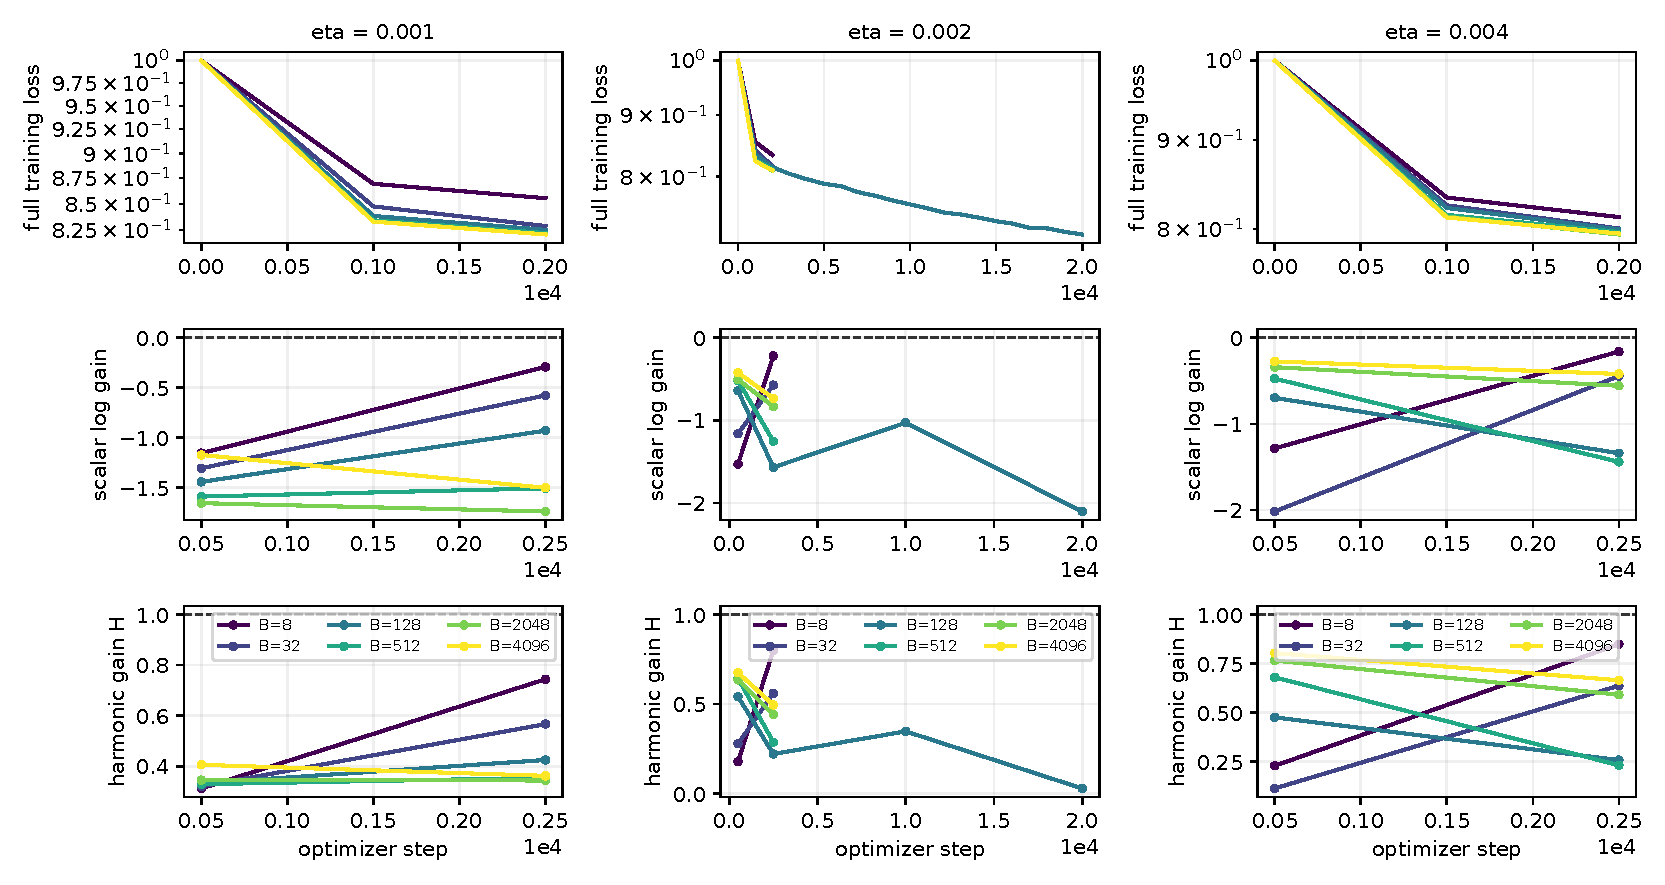
\includegraphics[width=\linewidth,height=0.78\textheight,keepaspectratio]{img/current_results/wrn_no_bn_04_dynamics.pdf}
\caption{\textbf{WideResNet-10-2, native Fixup | training and conditional gain dynamics.} Each batch curve averages run-level measurements at shared checkpoints and stops at the last common measurement. Loss and gain panels use their own recorded sampling grids. Finite training prefixes and decreasing loss do not establish a stationary distribution.}
\label{fig:current-wrn-no-bn-04-dynamics}
\end{figure}\clearpage

\begin{figure}[p]\centering
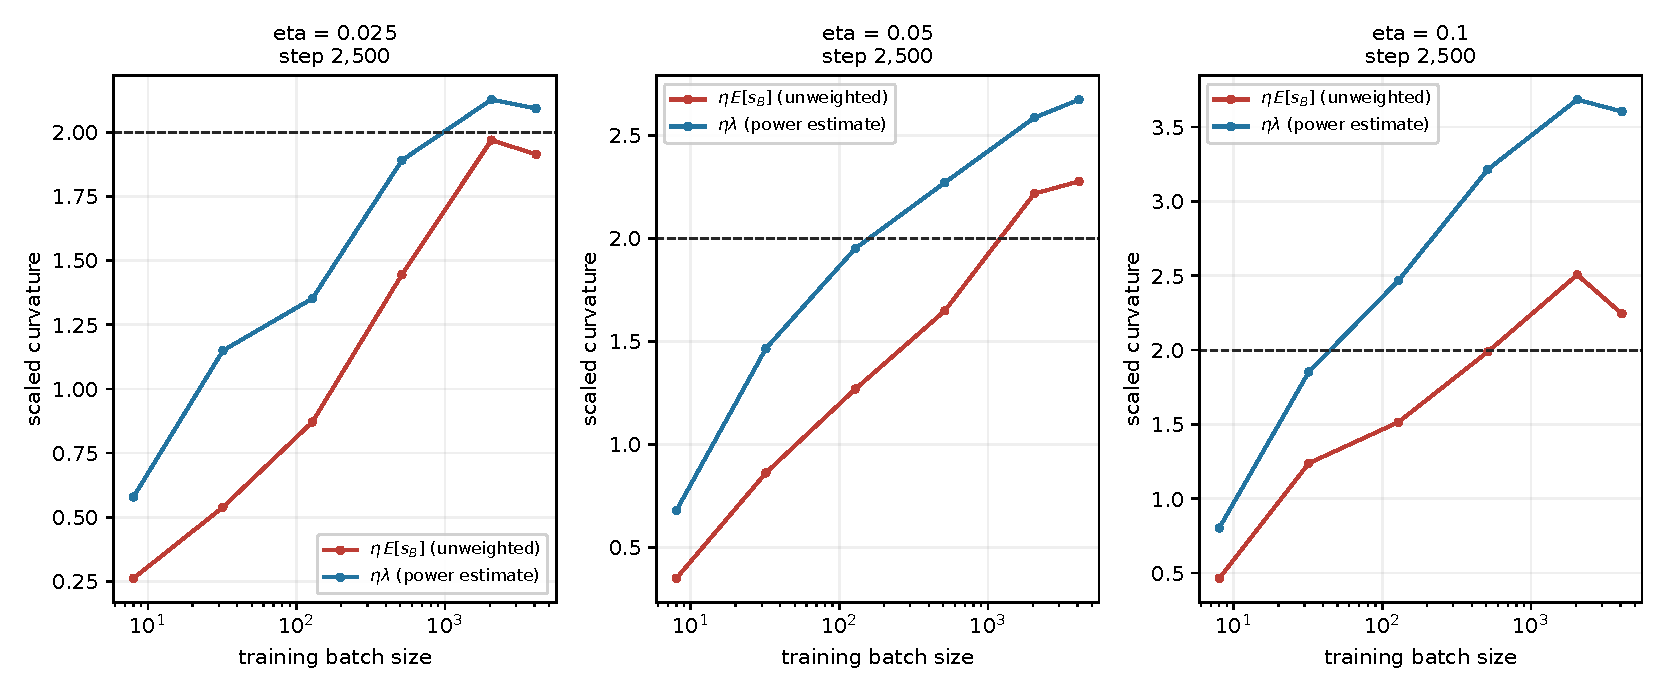
\includegraphics[width=\linewidth,height=0.78\textheight,keepaspectratio]{img/current_results/resnet32_01_curvature.pdf}
\caption{\textbf{ResNet-32 without BatchNorm | curvature thresholds.} eta=0.025: step 2,500; eta=0.05: step 2,500; eta=0.1: step 2,500. Curves show average run-level measurements. The Hessian curve is a finite power-iteration estimate; it is not a certified largest eigenvalue. Actual saved learning rates are used. A red cross retains a pre-escape checkpoint.}
\label{fig:current-resnet32-01-curvature}
\end{figure}\clearpage

\begin{figure}[p]\centering
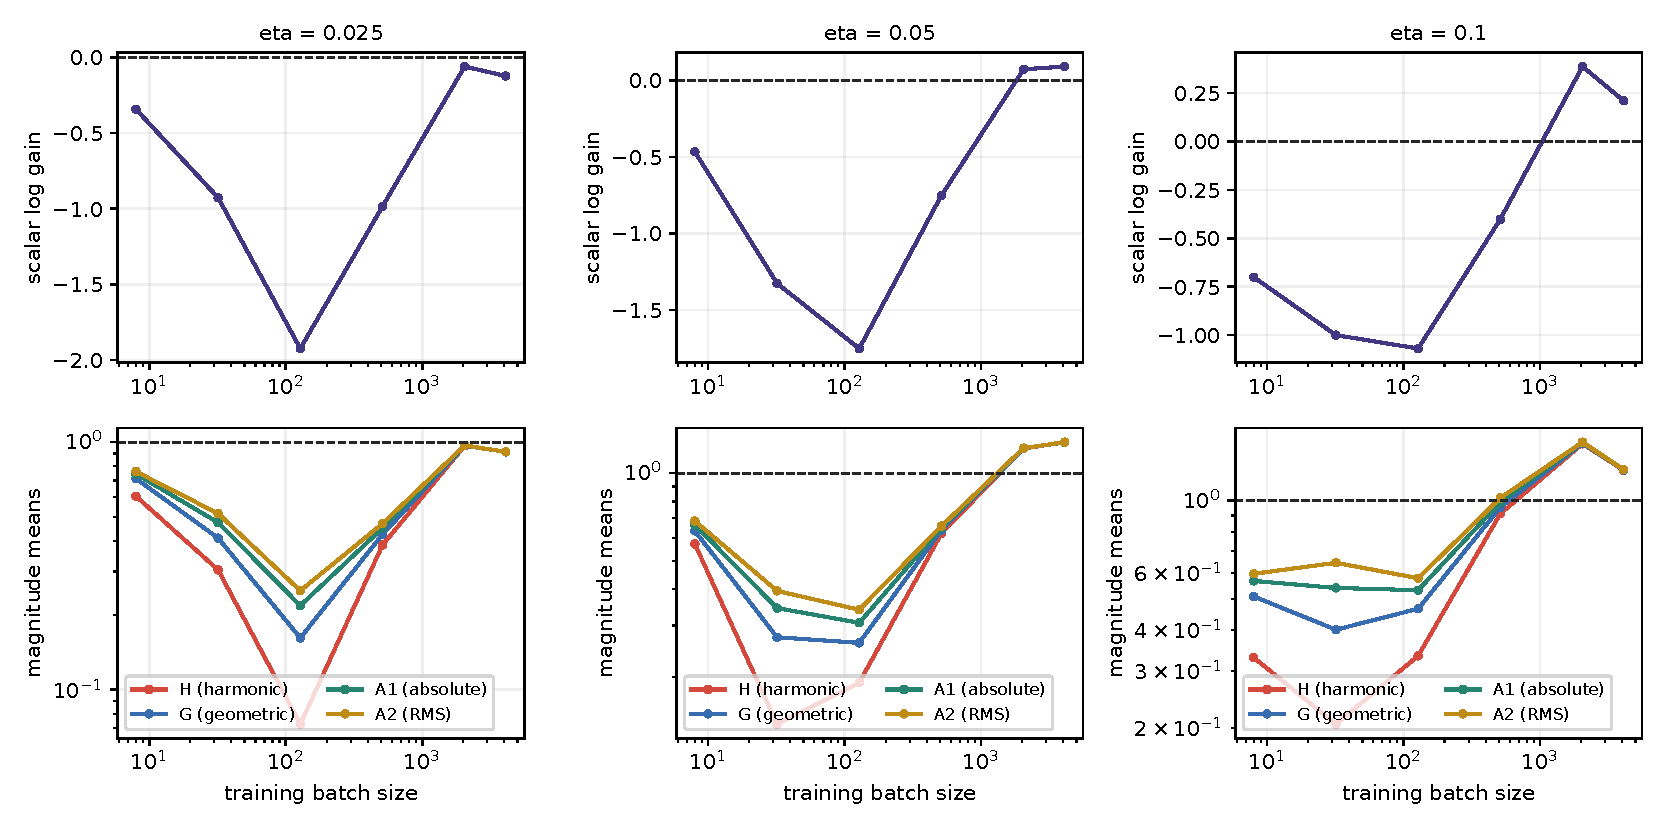
\includegraphics[width=\linewidth,height=0.78\textheight,keepaspectratio]{img/current_results/resnet32_02_moments.pdf}
\caption{\textbf{ResNet-32 without BatchNorm | the moment ladder.} eta=0.025: step 2,500; eta=0.05: step 2,500; eta=0.1: step 2,500. Curves show average run-level measurements. H=1/E[1/|a|], G=exp(Lambda), A1=E|a|, A2=sqrt(E|a|\textasciicircum{}2). The lower panel uses a logarithmic scale. A mean of run-level H estimates is not H of a pooled distribution; finite estimates do not prove inverse-moment existence.}
\label{fig:current-resnet32-02-moments}
\end{figure}\clearpage

\begin{figure}[p]\centering
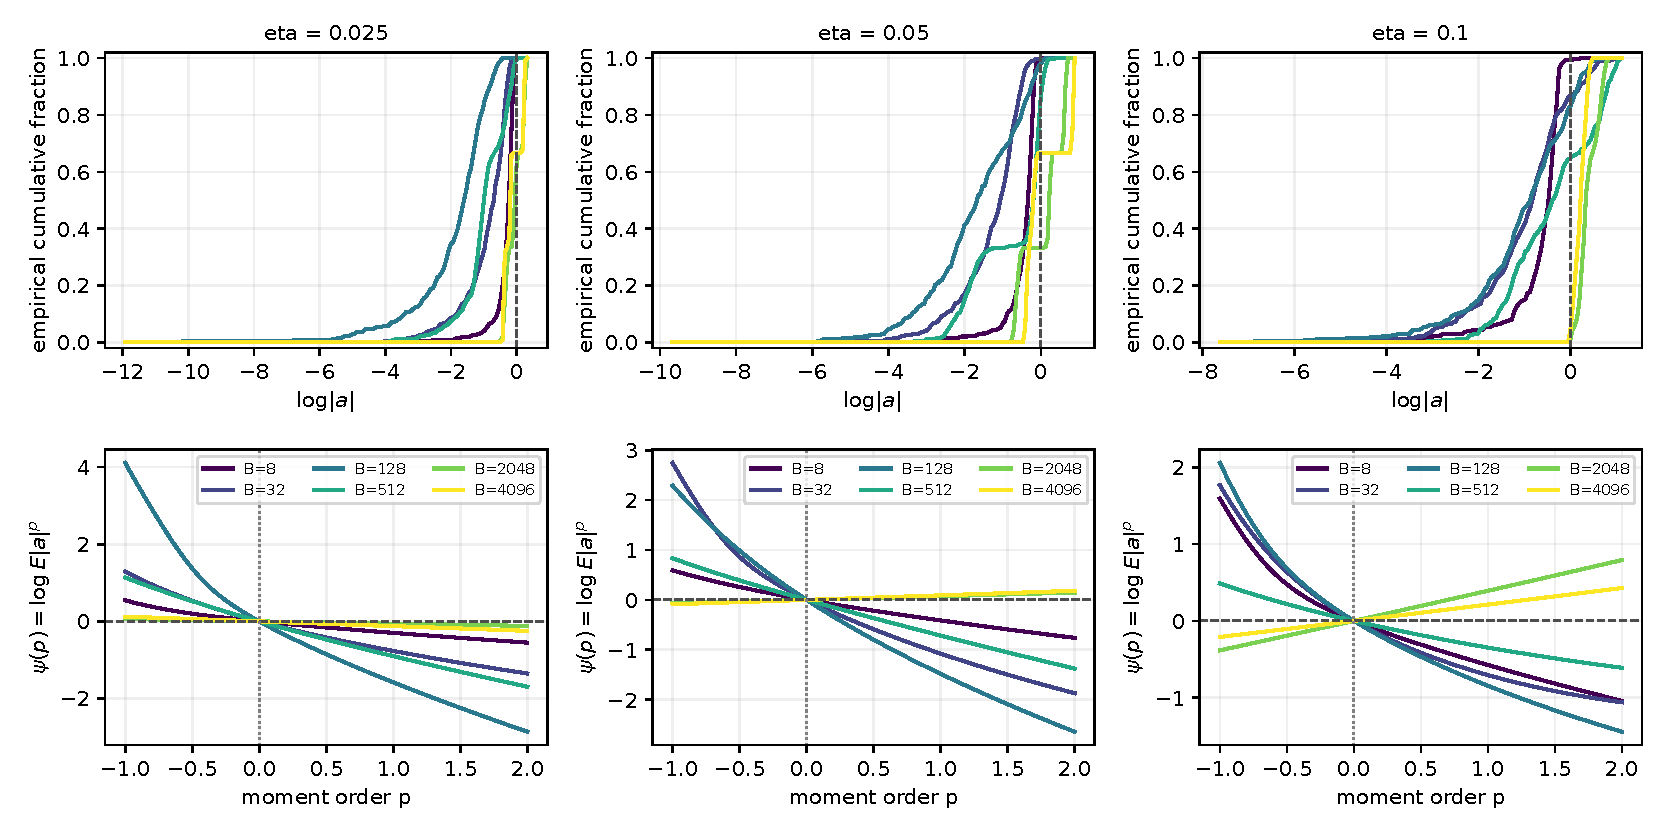
\includegraphics[width=\linewidth,height=0.78\textheight,keepaspectratio]{img/current_results/resnet32_03_gain_law.pdf}
\caption{\textbf{ResNet-32 without BatchNorm | gain distributions and moment pressure.} eta=0.025: step 2,500; eta=0.05: step 2,500; eta=0.1: step 2,500. Curves show average run-level measurements. CDFs and log moments are computed within each run, then averaged equally. These are distributions of a conditional scalar multiplier, not distributions of a fixed parameter coordinate. Values near a=0 dominate inverse moments; p=0 is exactly zero by definition.}
\label{fig:current-resnet32-03-gain-law}
\end{figure}\clearpage

\begin{figure}[p]\centering
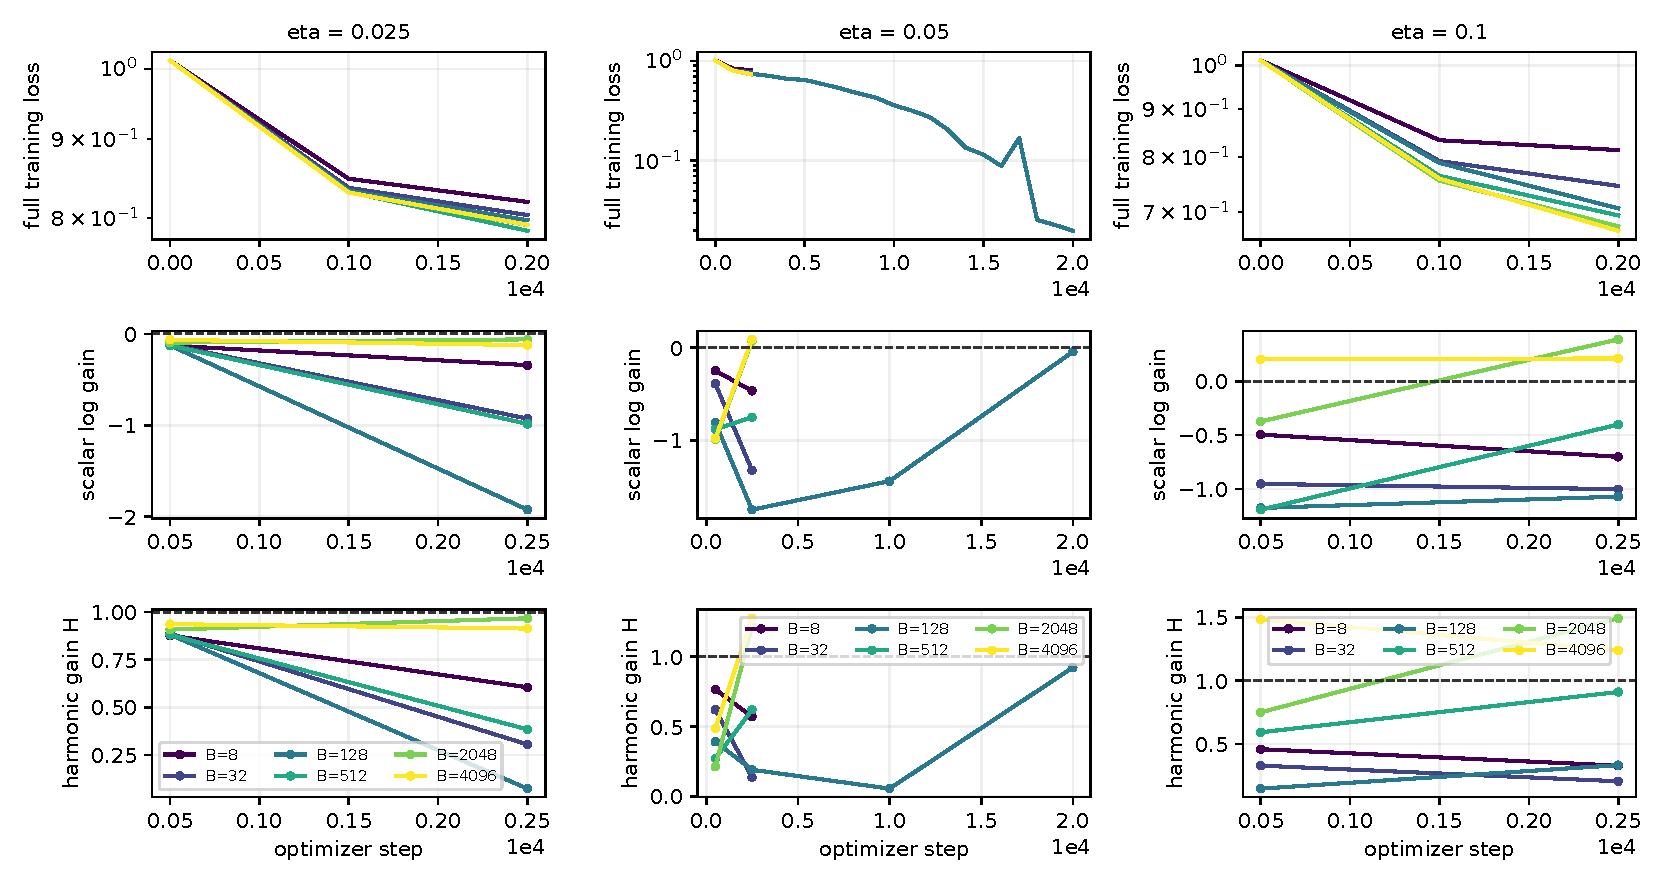
\includegraphics[width=\linewidth,height=0.78\textheight,keepaspectratio]{img/current_results/resnet32_04_dynamics.pdf}
\caption{\textbf{ResNet-32 without BatchNorm | training and conditional gain dynamics.} Each batch curve averages run-level measurements at shared checkpoints and stops at the last common measurement. Loss and gain panels use their own recorded sampling grids. Finite training prefixes and decreasing loss do not establish a stationary distribution.}
\label{fig:current-resnet32-04-dynamics}
\end{figure}\clearpage

\begin{figure}[p]\centering
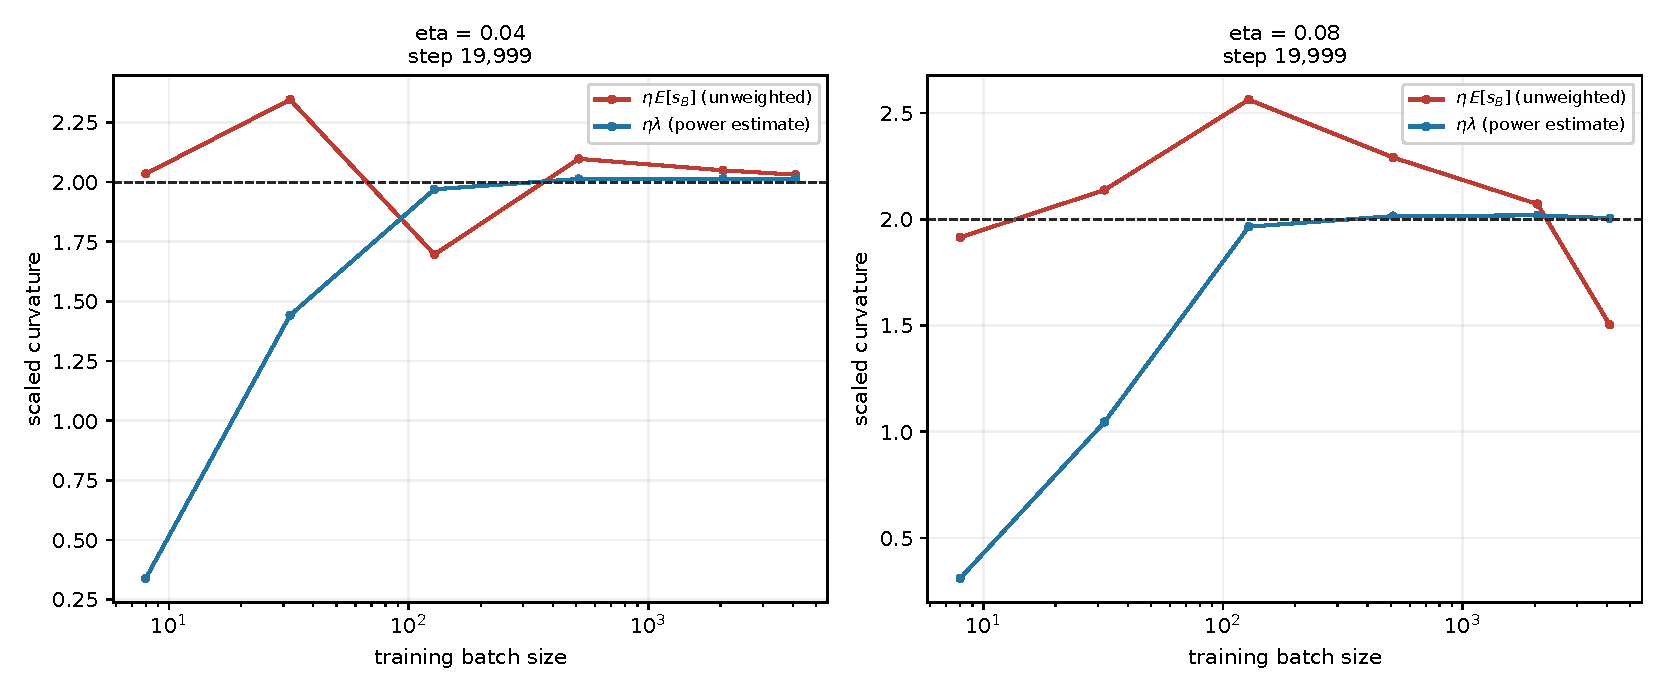
\includegraphics[width=\linewidth,height=0.78\textheight,keepaspectratio]{img/current_results/cnn_01_curvature.pdf}
\caption{\textbf{CNN, 3 convolutional layers (ReLU) | curvature thresholds.} eta=0.04: step 19,999; eta=0.08: step 19,999. Curves show average run-level measurements. The Hessian curve is a finite power-iteration estimate; it is not a certified largest eigenvalue. Actual saved learning rates are used. A red cross retains a pre-escape checkpoint.}
\label{fig:current-cnn-01-curvature}
\end{figure}\clearpage

\begin{figure}[p]\centering
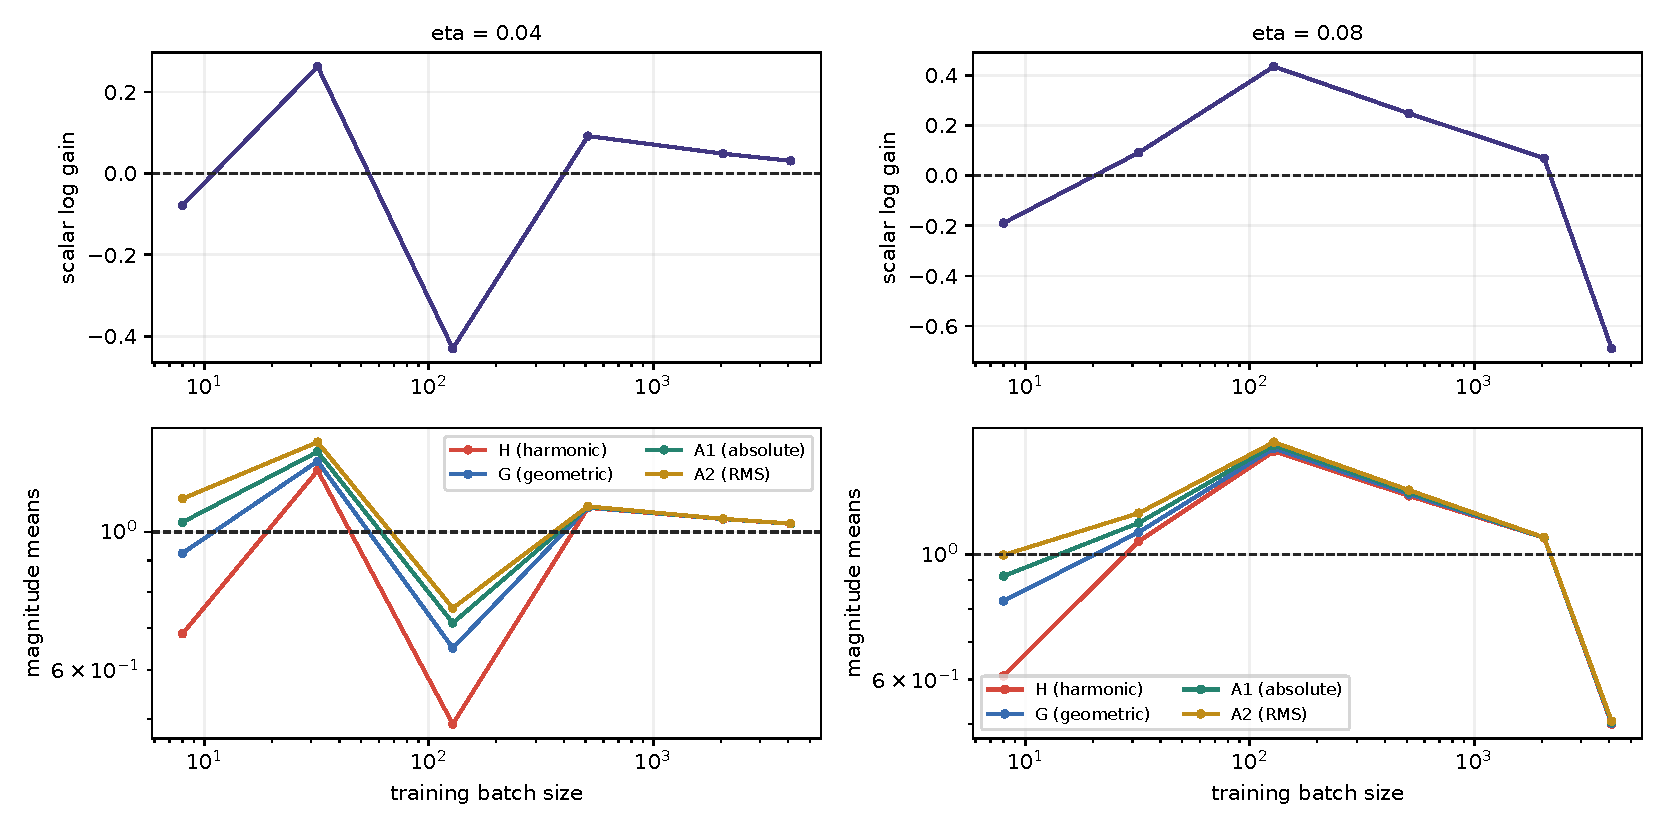
\includegraphics[width=\linewidth,height=0.78\textheight,keepaspectratio]{img/current_results/cnn_02_moments.pdf}
\caption{\textbf{CNN, 3 convolutional layers (ReLU) | the moment ladder.} eta=0.04: step 19,999; eta=0.08: step 19,999. Curves show average run-level measurements. H=1/E[1/|a|], G=exp(Lambda), A1=E|a|, A2=sqrt(E|a|\textasciicircum{}2). The lower panel uses a logarithmic scale. A mean of run-level H estimates is not H of a pooled distribution; finite estimates do not prove inverse-moment existence.}
\label{fig:current-cnn-02-moments}
\end{figure}\clearpage

\begin{figure}[p]\centering
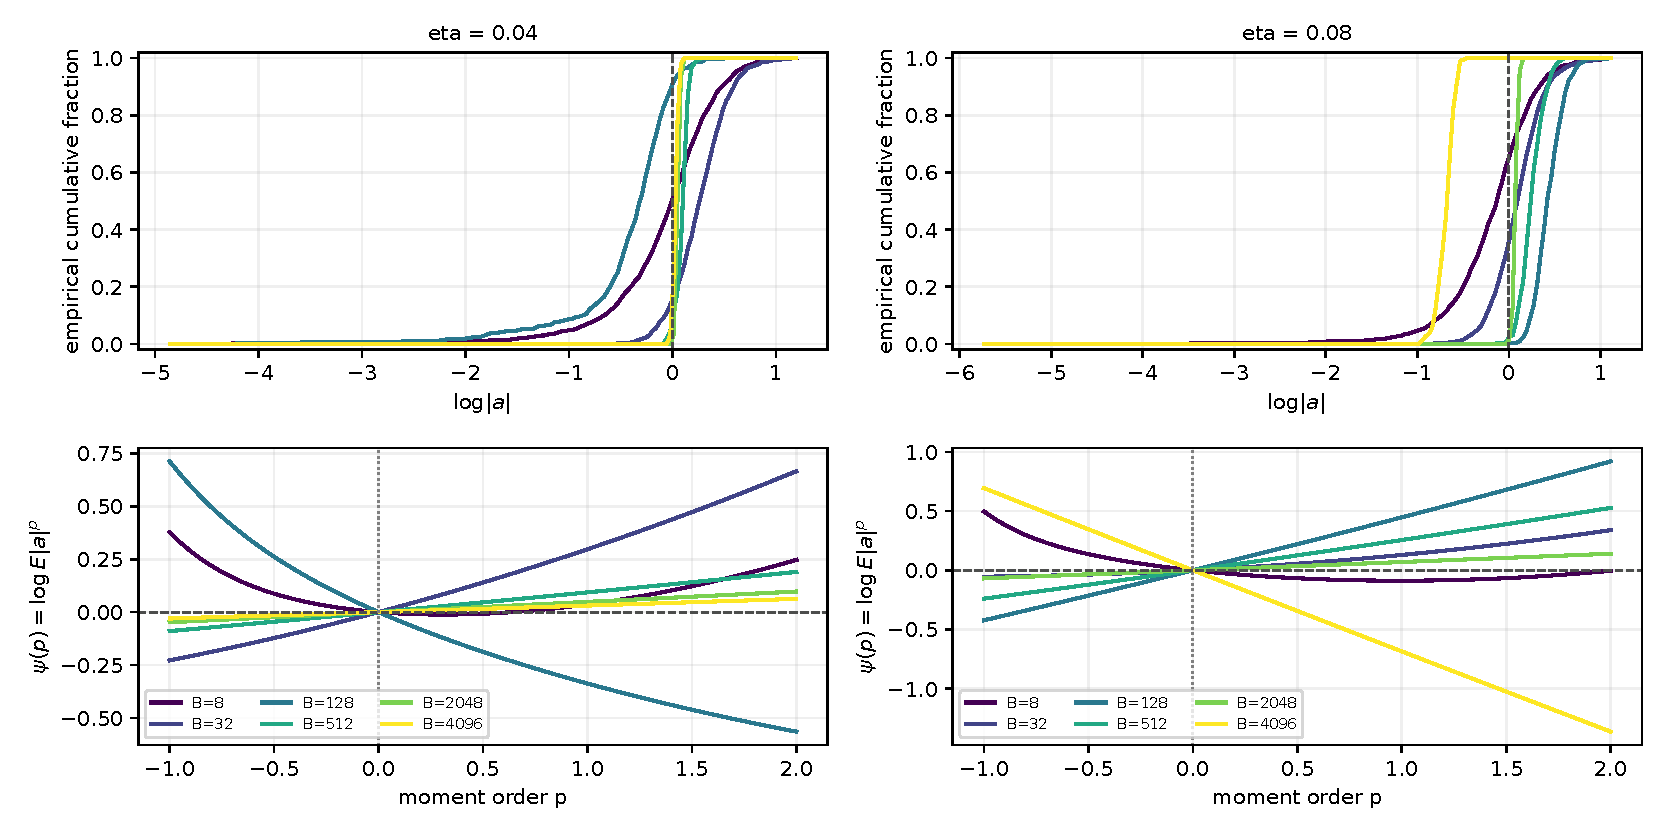
\includegraphics[width=\linewidth,height=0.78\textheight,keepaspectratio]{img/current_results/cnn_03_gain_law.pdf}
\caption{\textbf{CNN, 3 convolutional layers (ReLU) | gain distributions and moment pressure.} eta=0.04: step 19,999; eta=0.08: step 19,999. Curves show average run-level measurements. CDFs and log moments are computed within each run, then averaged equally. These are distributions of a conditional scalar multiplier, not distributions of a fixed parameter coordinate. Values near a=0 dominate inverse moments; p=0 is exactly zero by definition.}
\label{fig:current-cnn-03-gain-law}
\end{figure}\clearpage

\begin{figure}[p]\centering
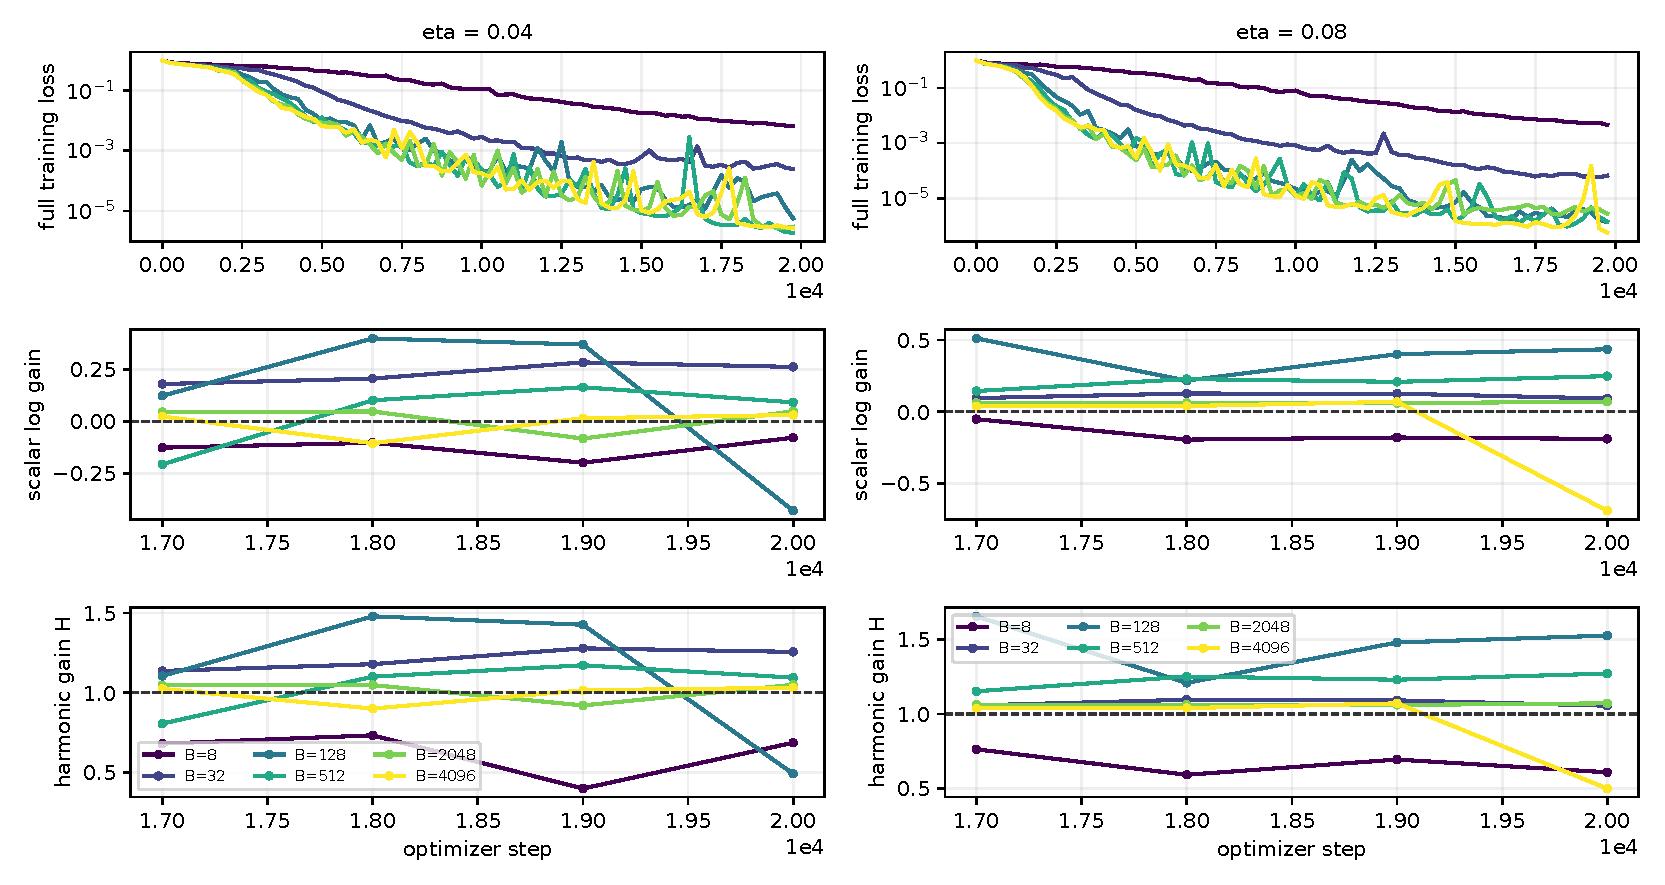
\includegraphics[width=\linewidth,height=0.78\textheight,keepaspectratio]{img/current_results/cnn_04_dynamics.pdf}
\caption{\textbf{CNN, 3 convolutional layers (ReLU) | training and conditional gain dynamics.} Each batch curve averages run-level measurements at shared checkpoints and stops at the last common measurement. Loss and gain panels use their own recorded sampling grids. Finite training prefixes and decreasing loss do not establish a stationary distribution.}
\label{fig:current-cnn-04-dynamics}
\end{figure}\clearpage

\begin{figure}[p]\centering
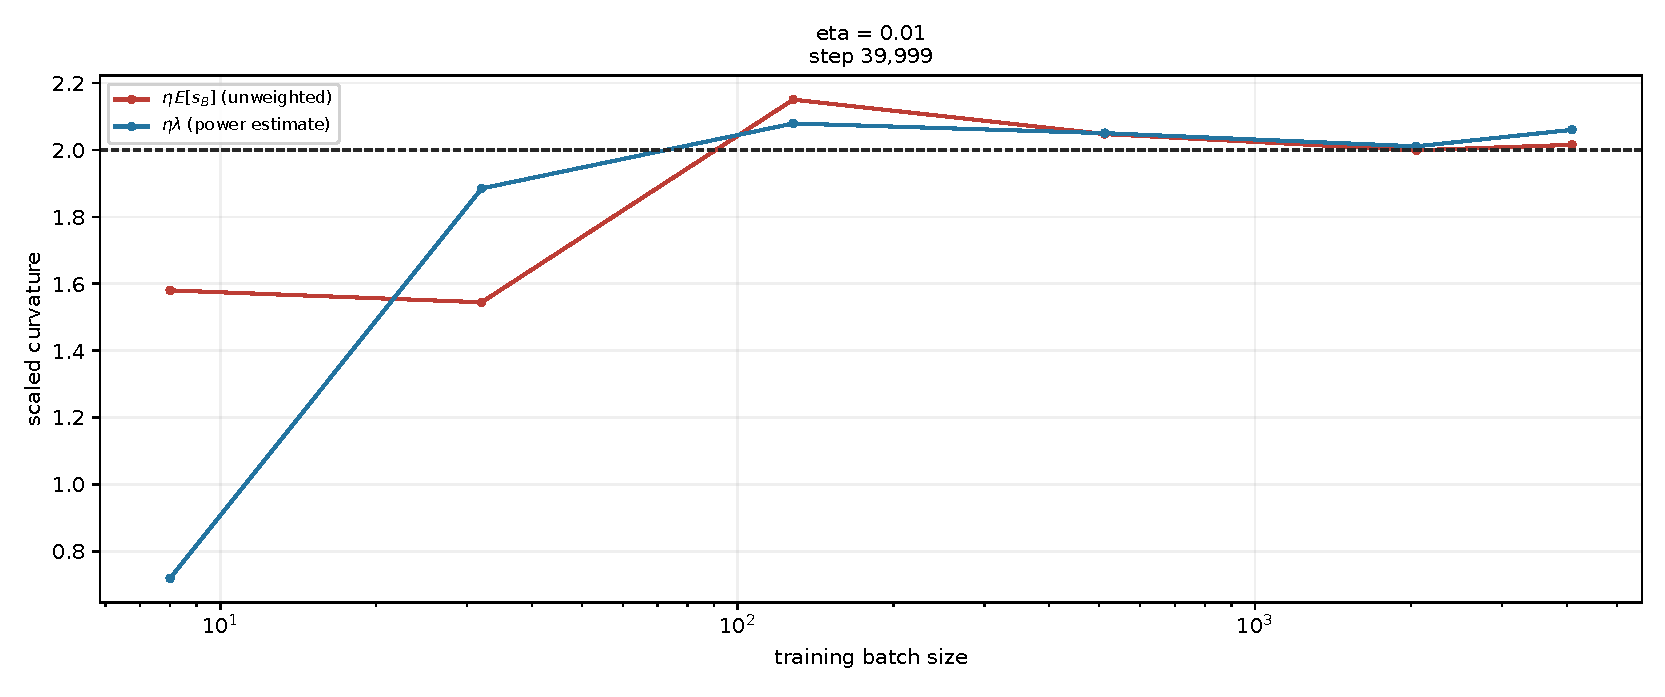
\includegraphics[width=\linewidth,height=0.78\textheight,keepaspectratio]{img/current_results/mlp_d1_01_curvature.pdf}
\caption{\textbf{MLP, 1 x 256 (ReLU) | curvature thresholds.} eta=0.01: step 39,999. Curves show average run-level measurements. The Hessian curve is a finite power-iteration estimate; it is not a certified largest eigenvalue. Actual saved learning rates are used. A red cross retains a pre-escape checkpoint.}
\label{fig:current-mlp-d1-01-curvature}
\end{figure}\clearpage

\begin{figure}[p]\centering
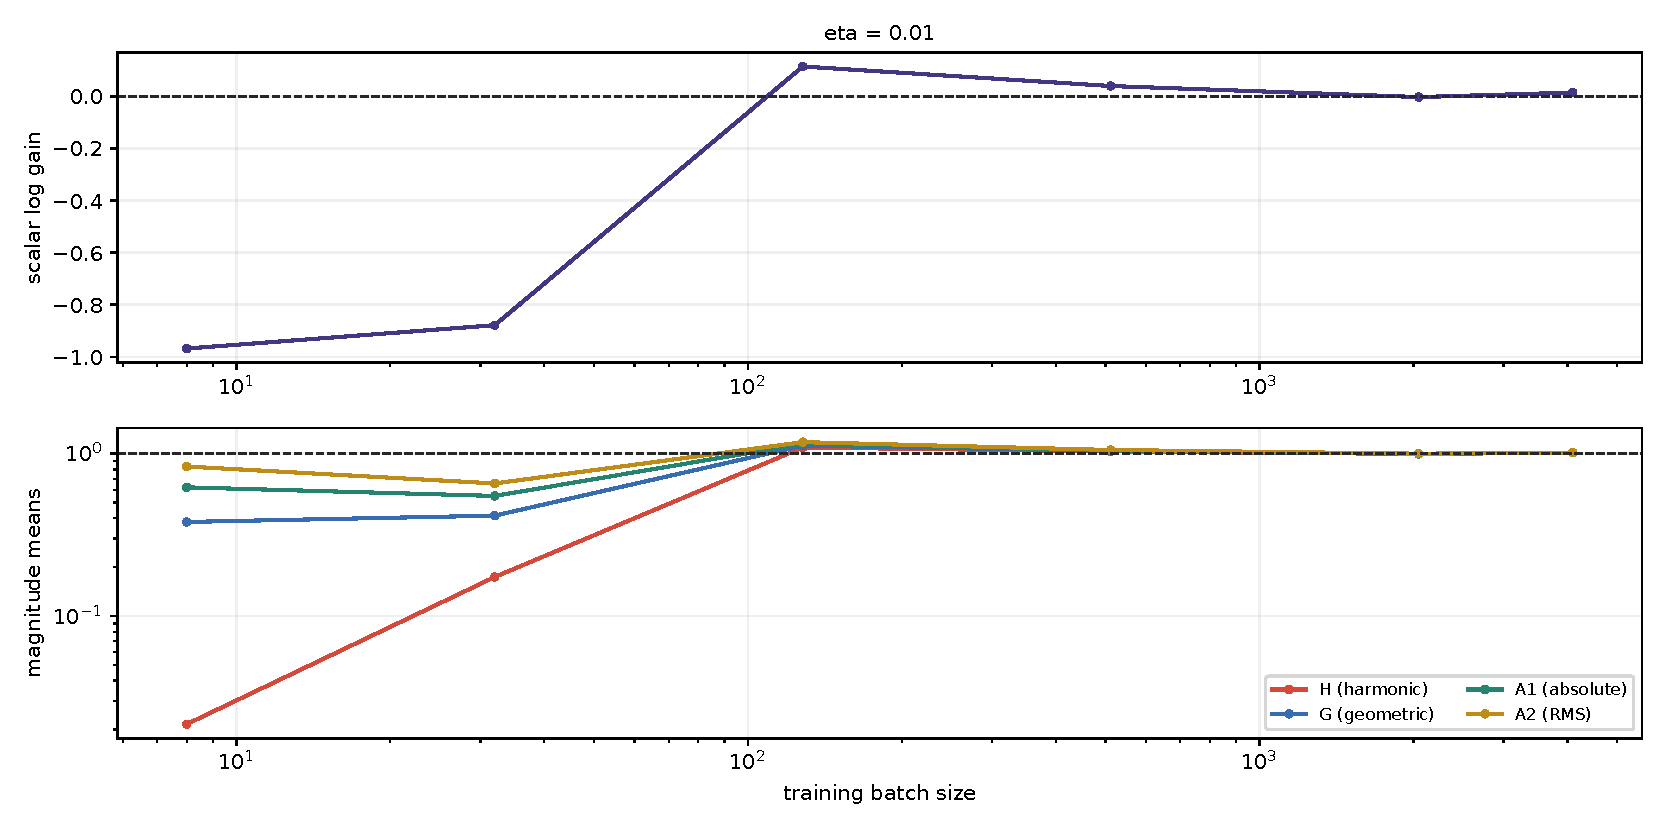
\includegraphics[width=\linewidth,height=0.78\textheight,keepaspectratio]{img/current_results/mlp_d1_02_moments.pdf}
\caption{\textbf{MLP, 1 x 256 (ReLU) | the moment ladder.} eta=0.01: step 39,999. Curves show average run-level measurements. H=1/E[1/|a|], G=exp(Lambda), A1=E|a|, A2=sqrt(E|a|\textasciicircum{}2). The lower panel uses a logarithmic scale. A mean of run-level H estimates is not H of a pooled distribution; finite estimates do not prove inverse-moment existence.}
\label{fig:current-mlp-d1-02-moments}
\end{figure}\clearpage

\begin{figure}[p]\centering
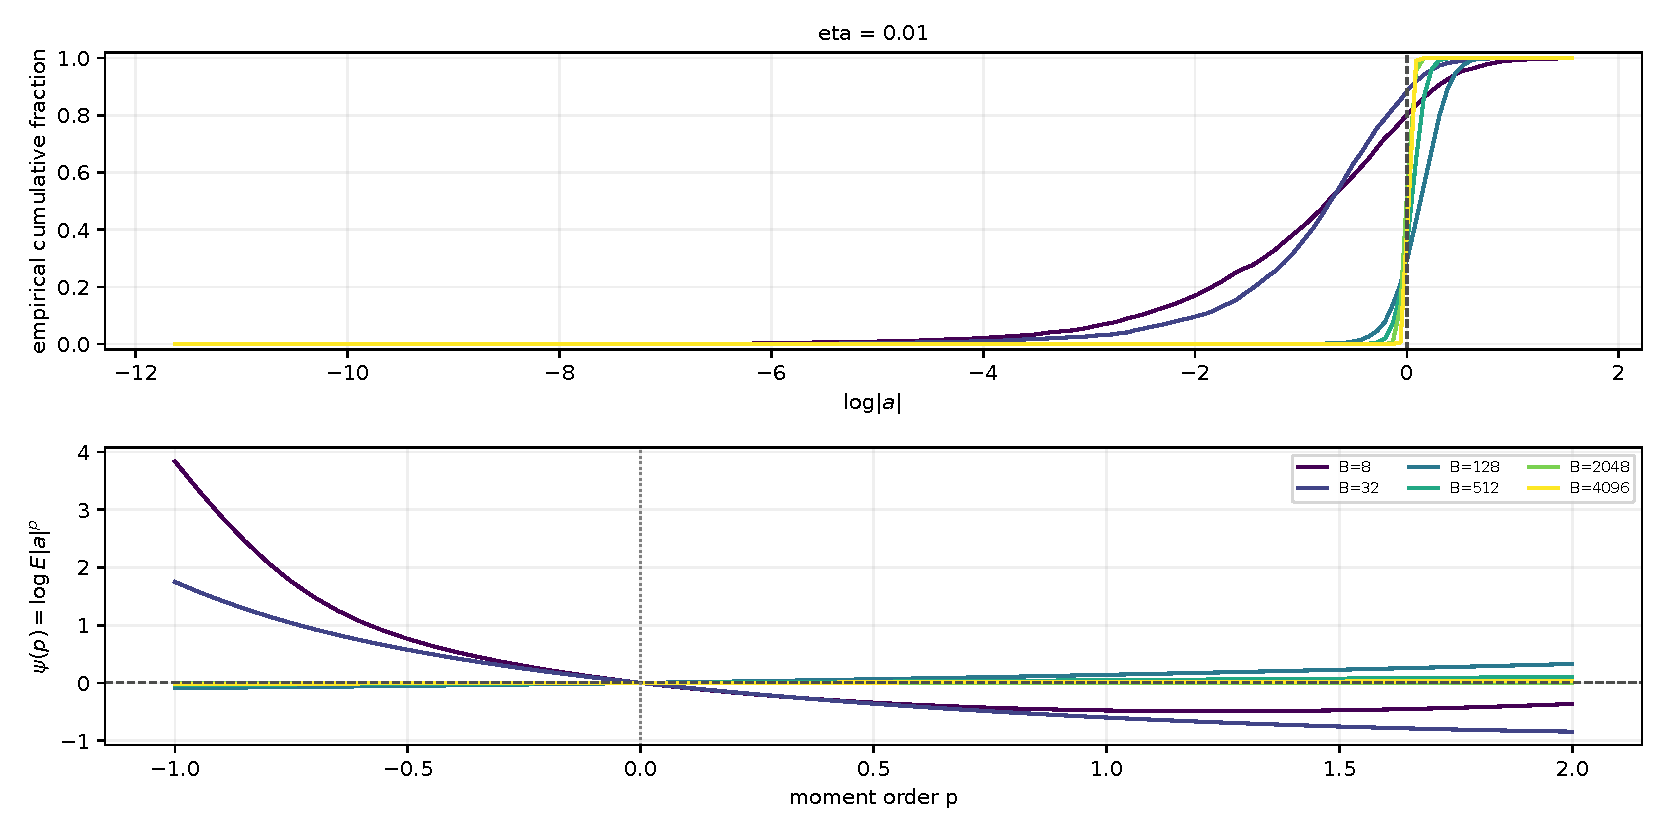
\includegraphics[width=\linewidth,height=0.78\textheight,keepaspectratio]{img/current_results/mlp_d1_03_gain_law.pdf}
\caption{\textbf{MLP, 1 x 256 (ReLU) | gain distributions and moment pressure.} eta=0.01: step 39,999. Curves show average run-level measurements. CDFs and log moments are computed within each run, then averaged equally. These are distributions of a conditional scalar multiplier, not distributions of a fixed parameter coordinate. Values near a=0 dominate inverse moments; p=0 is exactly zero by definition.}
\label{fig:current-mlp-d1-03-gain-law}
\end{figure}\clearpage

\begin{figure}[p]\centering
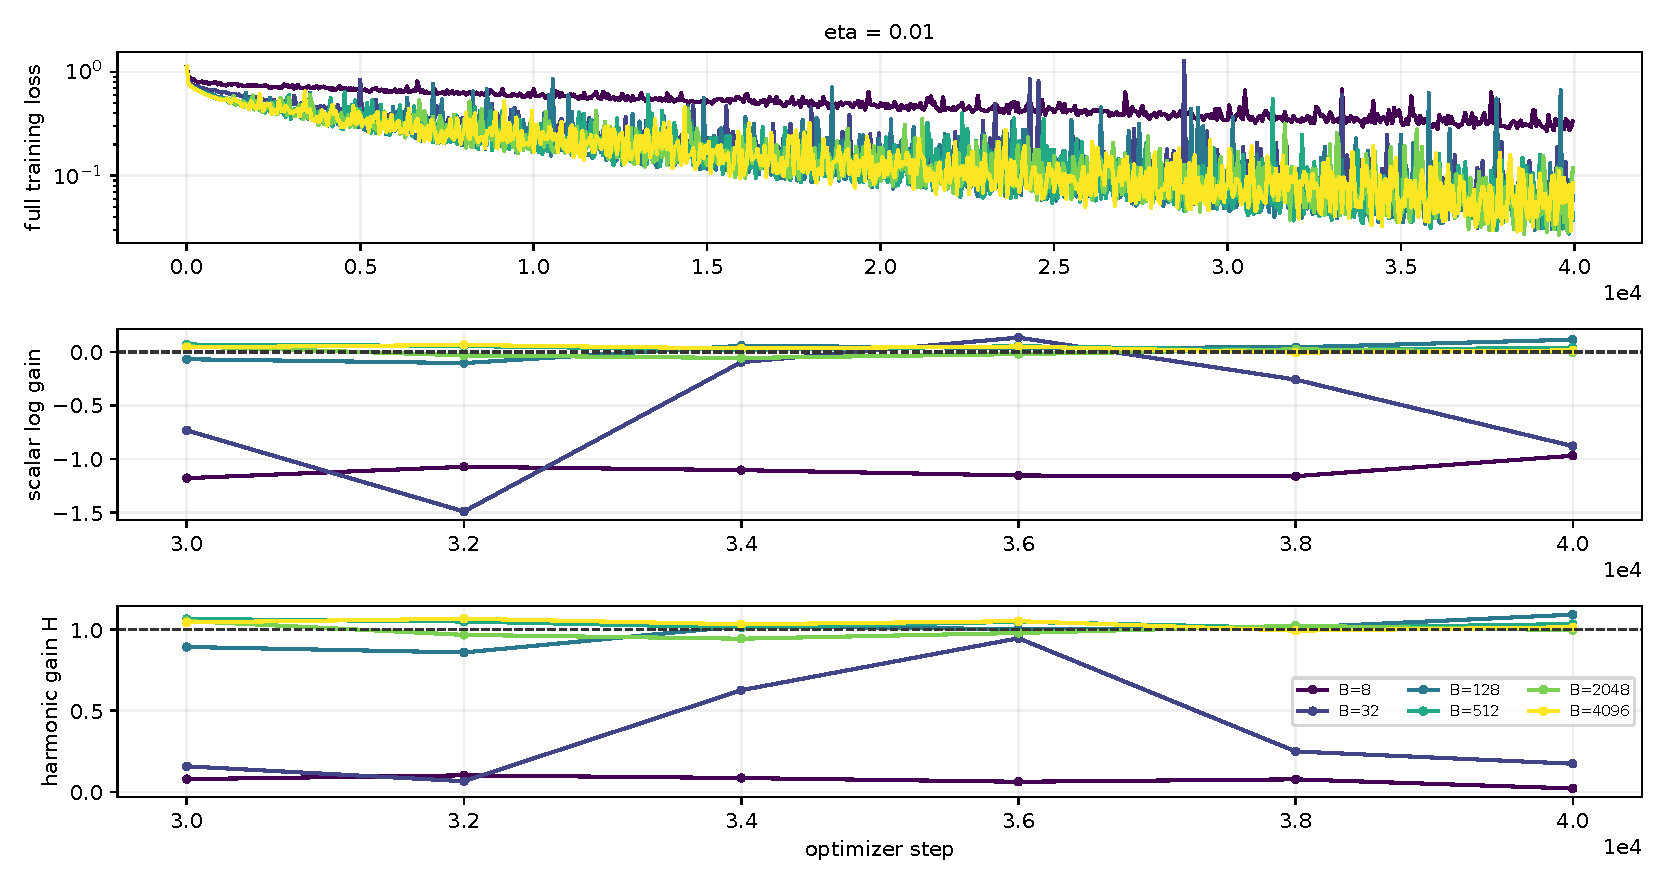
\includegraphics[width=\linewidth,height=0.78\textheight,keepaspectratio]{img/current_results/mlp_d1_04_dynamics.pdf}
\caption{\textbf{MLP, 1 x 256 (ReLU) | training and conditional gain dynamics.} Each batch curve averages run-level measurements at shared checkpoints and stops at the last common measurement. Loss and gain panels use their own recorded sampling grids. Finite training prefixes and decreasing loss do not establish a stationary distribution.}
\label{fig:current-mlp-d1-04-dynamics}
\end{figure}\clearpage

\begin{figure}[p]\centering
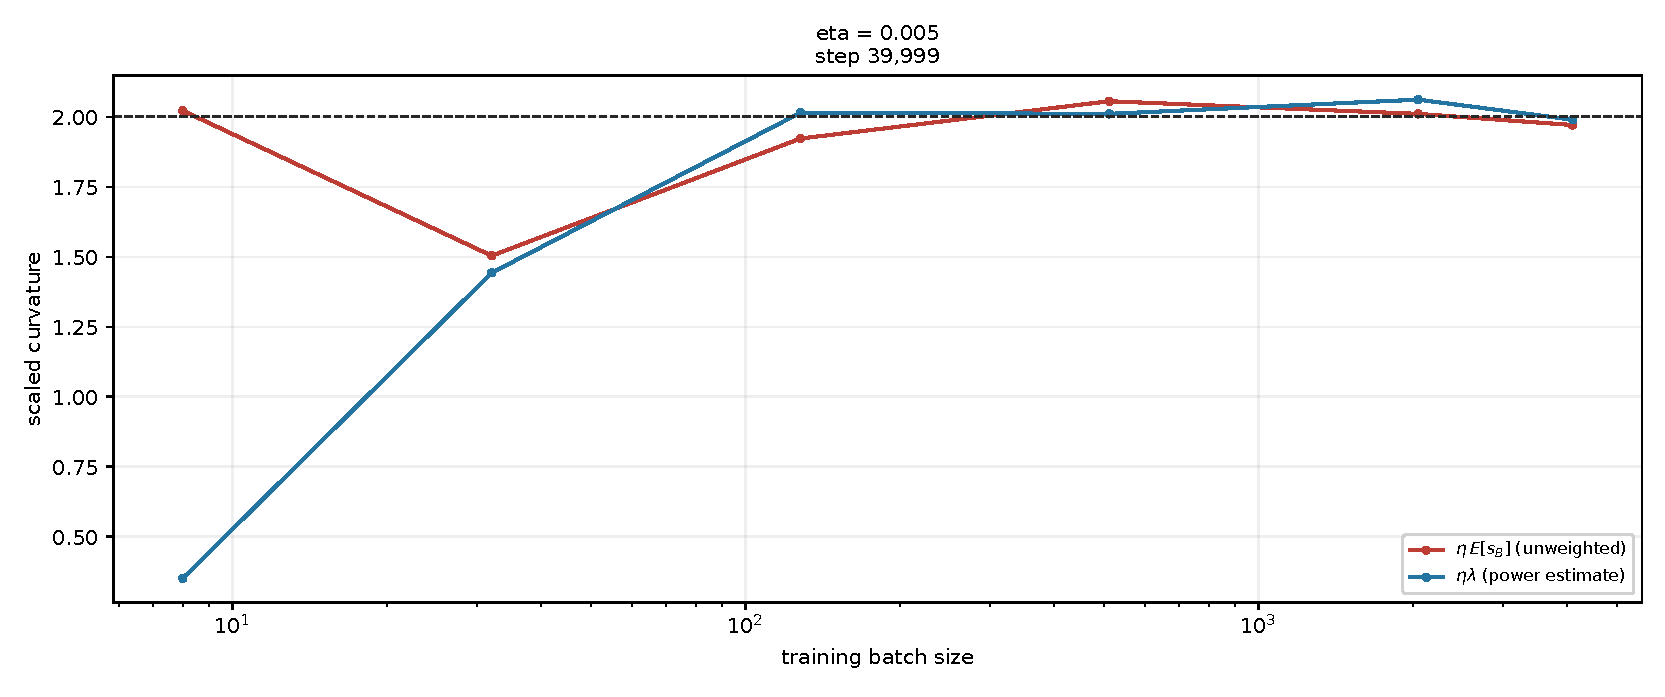
\includegraphics[width=\linewidth,height=0.78\textheight,keepaspectratio]{img/current_results/mlp_d2_01_curvature.pdf}
\caption{\textbf{MLP, 2 x 512 (ReLU) | curvature thresholds.} eta=0.005: step 39,999. Curves show average run-level measurements. The Hessian curve is a finite power-iteration estimate; it is not a certified largest eigenvalue. Actual saved learning rates are used. A red cross retains a pre-escape checkpoint.}
\label{fig:current-mlp-d2-01-curvature}
\end{figure}\clearpage

\begin{figure}[p]\centering
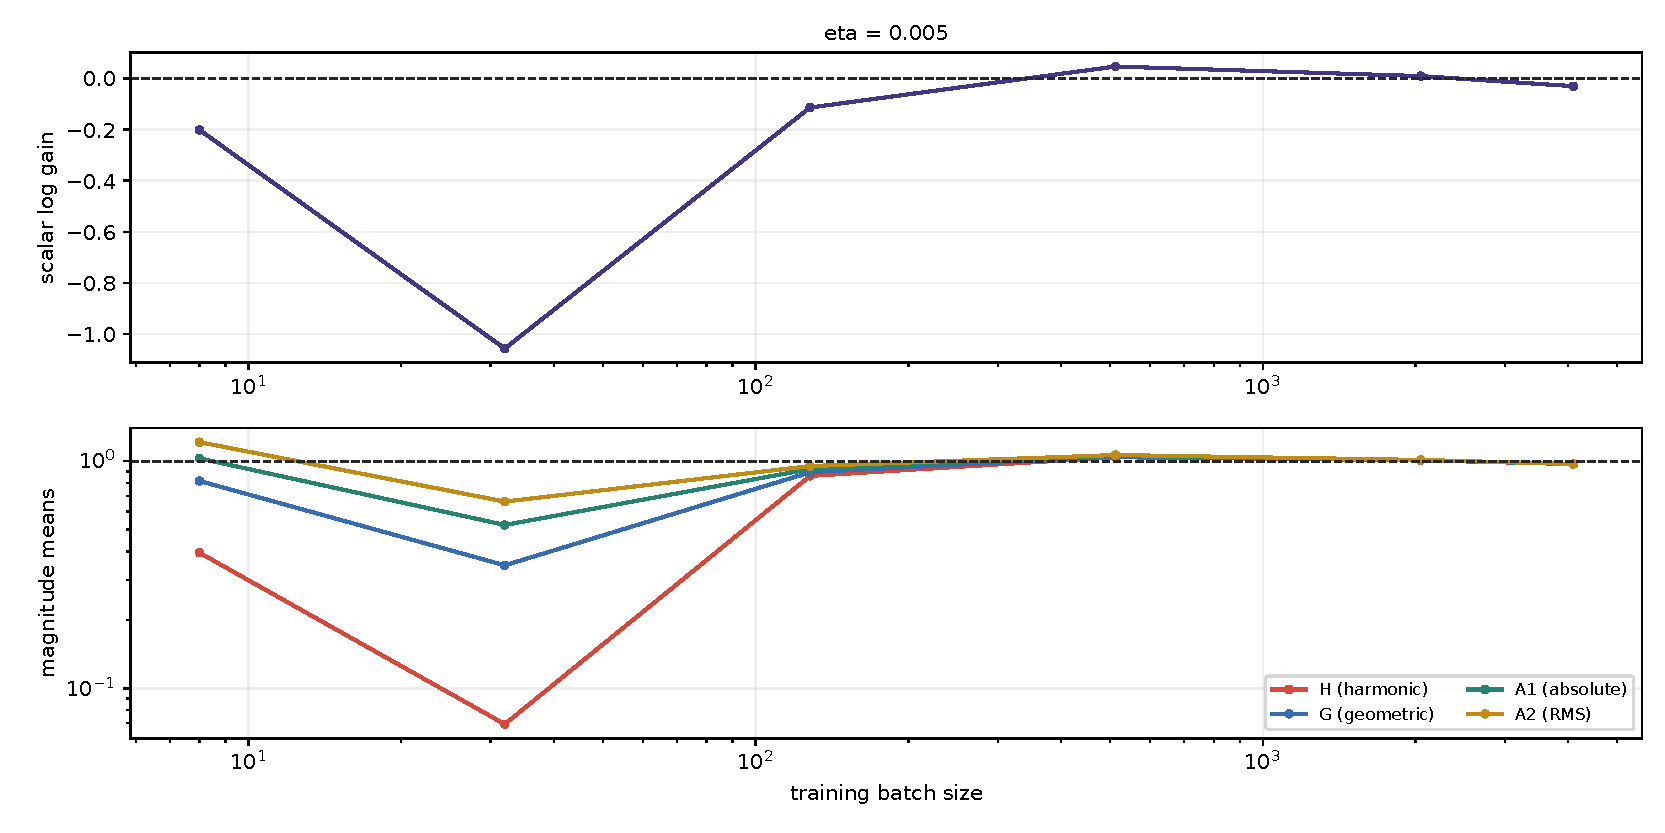
\includegraphics[width=\linewidth,height=0.78\textheight,keepaspectratio]{img/current_results/mlp_d2_02_moments.pdf}
\caption{\textbf{MLP, 2 x 512 (ReLU) | the moment ladder.} eta=0.005: step 39,999. Curves show average run-level measurements. H=1/E[1/|a|], G=exp(Lambda), A1=E|a|, A2=sqrt(E|a|\textasciicircum{}2). The lower panel uses a logarithmic scale. A mean of run-level H estimates is not H of a pooled distribution; finite estimates do not prove inverse-moment existence.}
\label{fig:current-mlp-d2-02-moments}
\end{figure}\clearpage

\begin{figure}[p]\centering
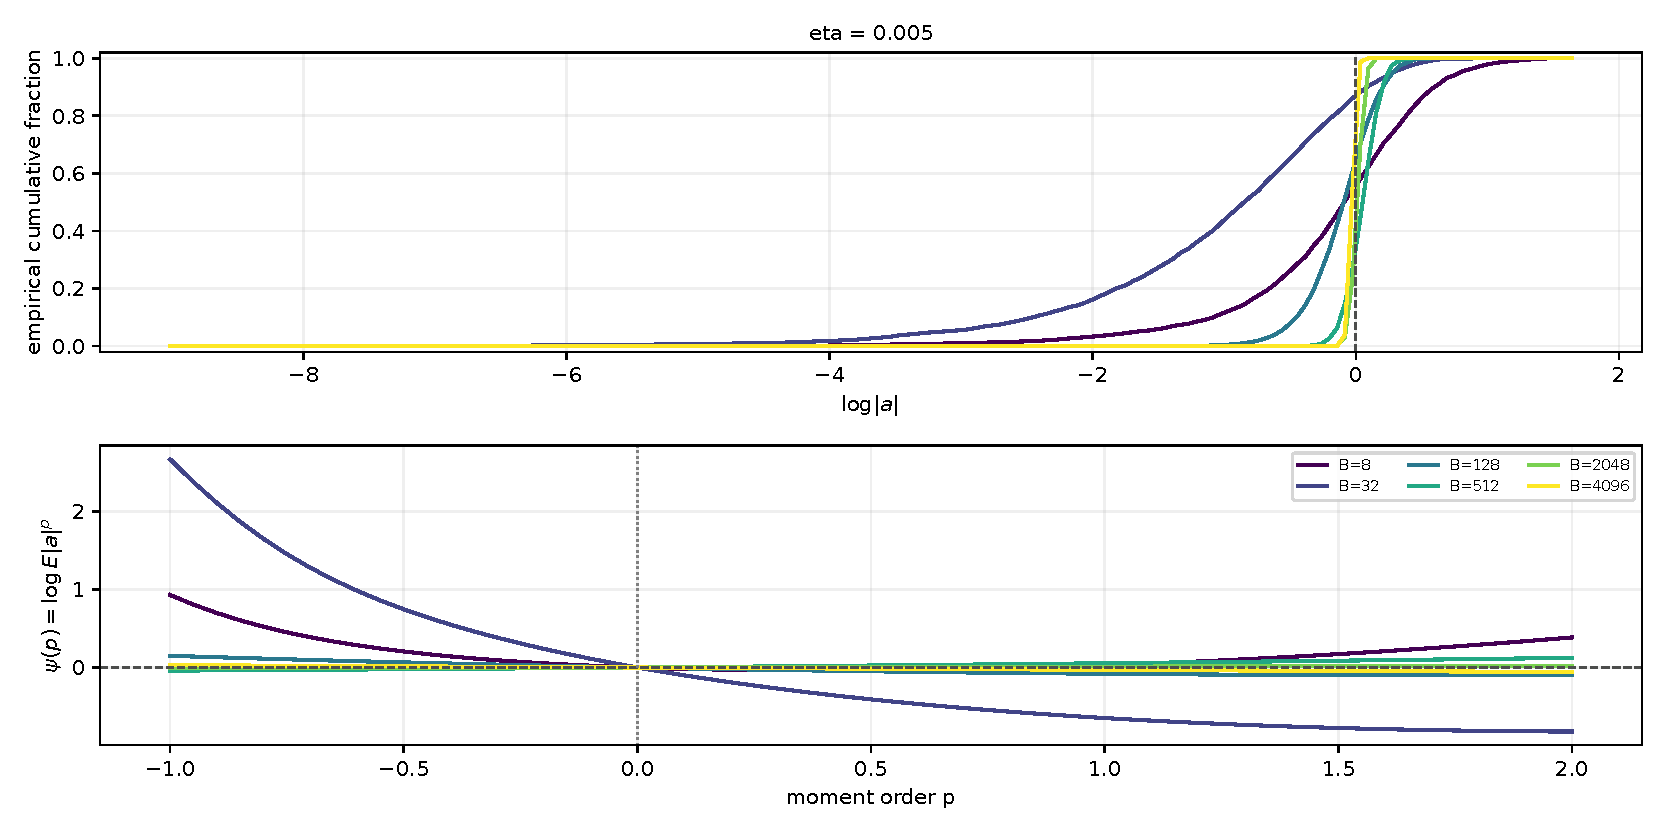
\includegraphics[width=\linewidth,height=0.78\textheight,keepaspectratio]{img/current_results/mlp_d2_03_gain_law.pdf}
\caption{\textbf{MLP, 2 x 512 (ReLU) | gain distributions and moment pressure.} eta=0.005: step 39,999. Curves show average run-level measurements. CDFs and log moments are computed within each run, then averaged equally. These are distributions of a conditional scalar multiplier, not distributions of a fixed parameter coordinate. Values near a=0 dominate inverse moments; p=0 is exactly zero by definition.}
\label{fig:current-mlp-d2-03-gain-law}
\end{figure}\clearpage

\begin{figure}[p]\centering
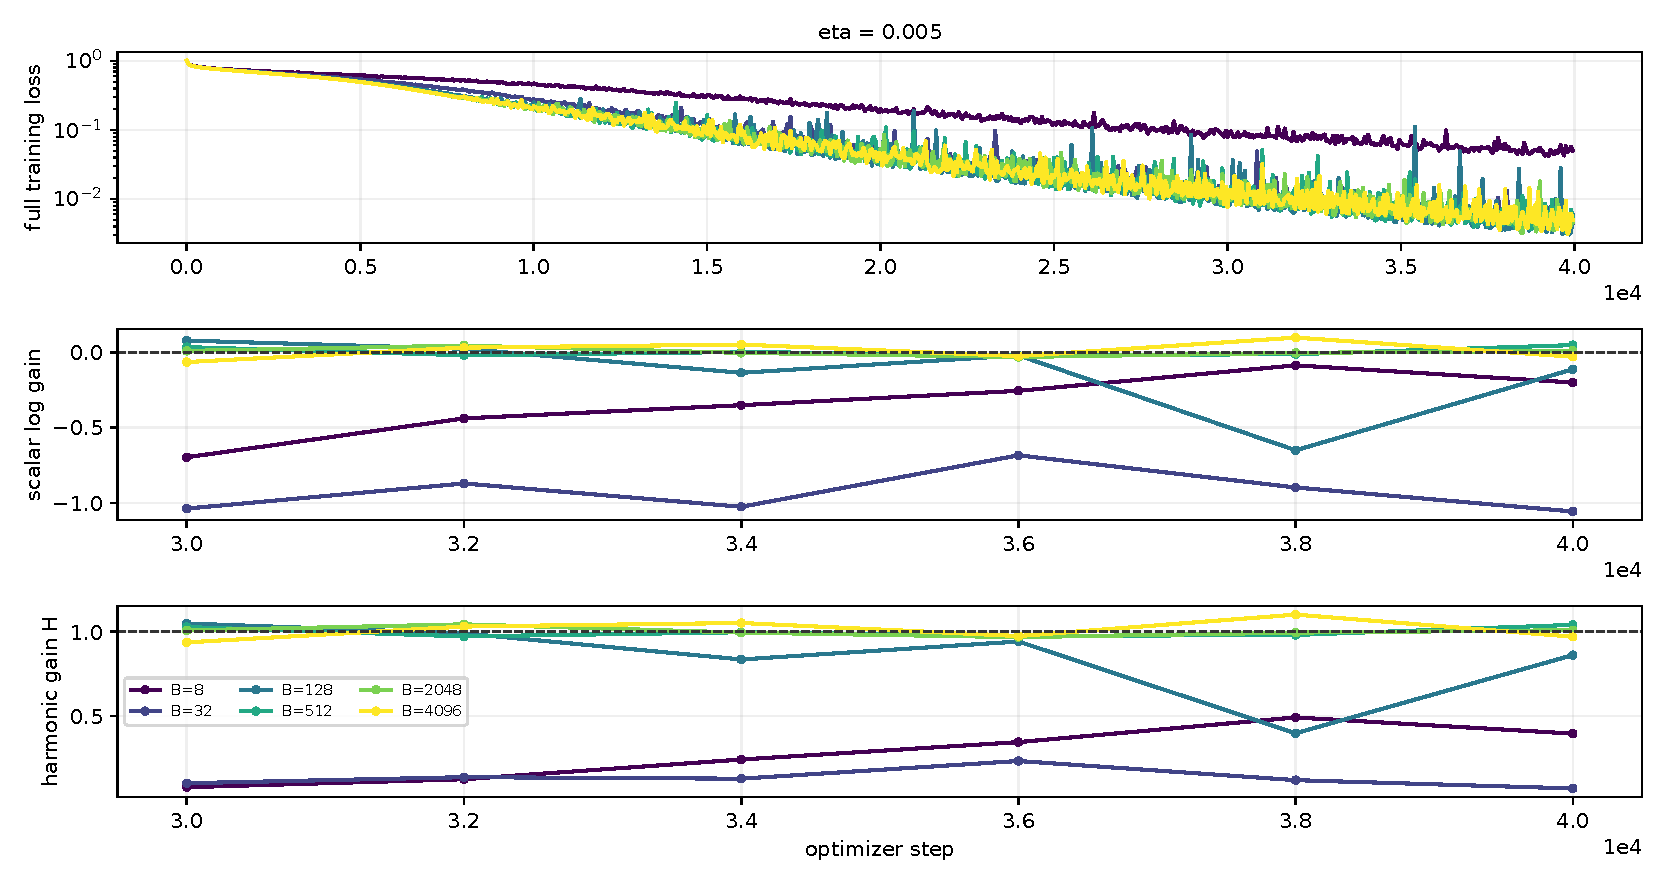
\includegraphics[width=\linewidth,height=0.78\textheight,keepaspectratio]{img/current_results/mlp_d2_04_dynamics.pdf}
\caption{\textbf{MLP, 2 x 512 (ReLU) | training and conditional gain dynamics.} Each batch curve averages run-level measurements at shared checkpoints and stops at the last common measurement. Loss and gain panels use their own recorded sampling grids. Finite training prefixes and decreasing loss do not establish a stationary distribution.}
\label{fig:current-mlp-d2-04-dynamics}
\end{figure}\clearpage

\begin{figure}[p]\centering
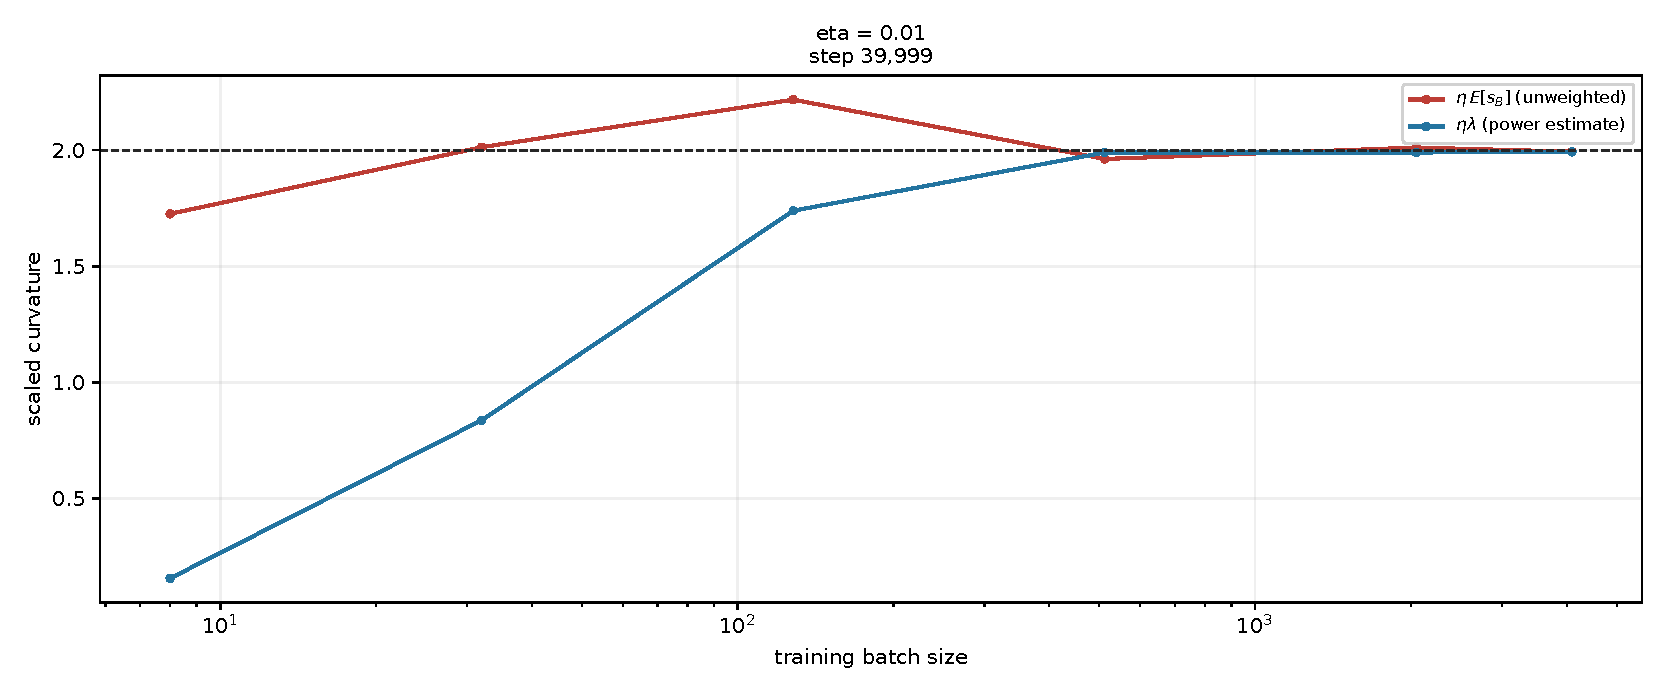
\includegraphics[width=\linewidth,height=0.78\textheight,keepaspectratio]{img/current_results/mlp_d3_01_curvature.pdf}
\caption{\textbf{MLP, 3 x 256 (ReLU) | curvature thresholds.} eta=0.01: step 39,999. Curves show average run-level measurements. The Hessian curve is a finite power-iteration estimate; it is not a certified largest eigenvalue. Actual saved learning rates are used. A red cross retains a pre-escape checkpoint.}
\label{fig:current-mlp-d3-01-curvature}
\end{figure}\clearpage

\begin{figure}[p]\centering
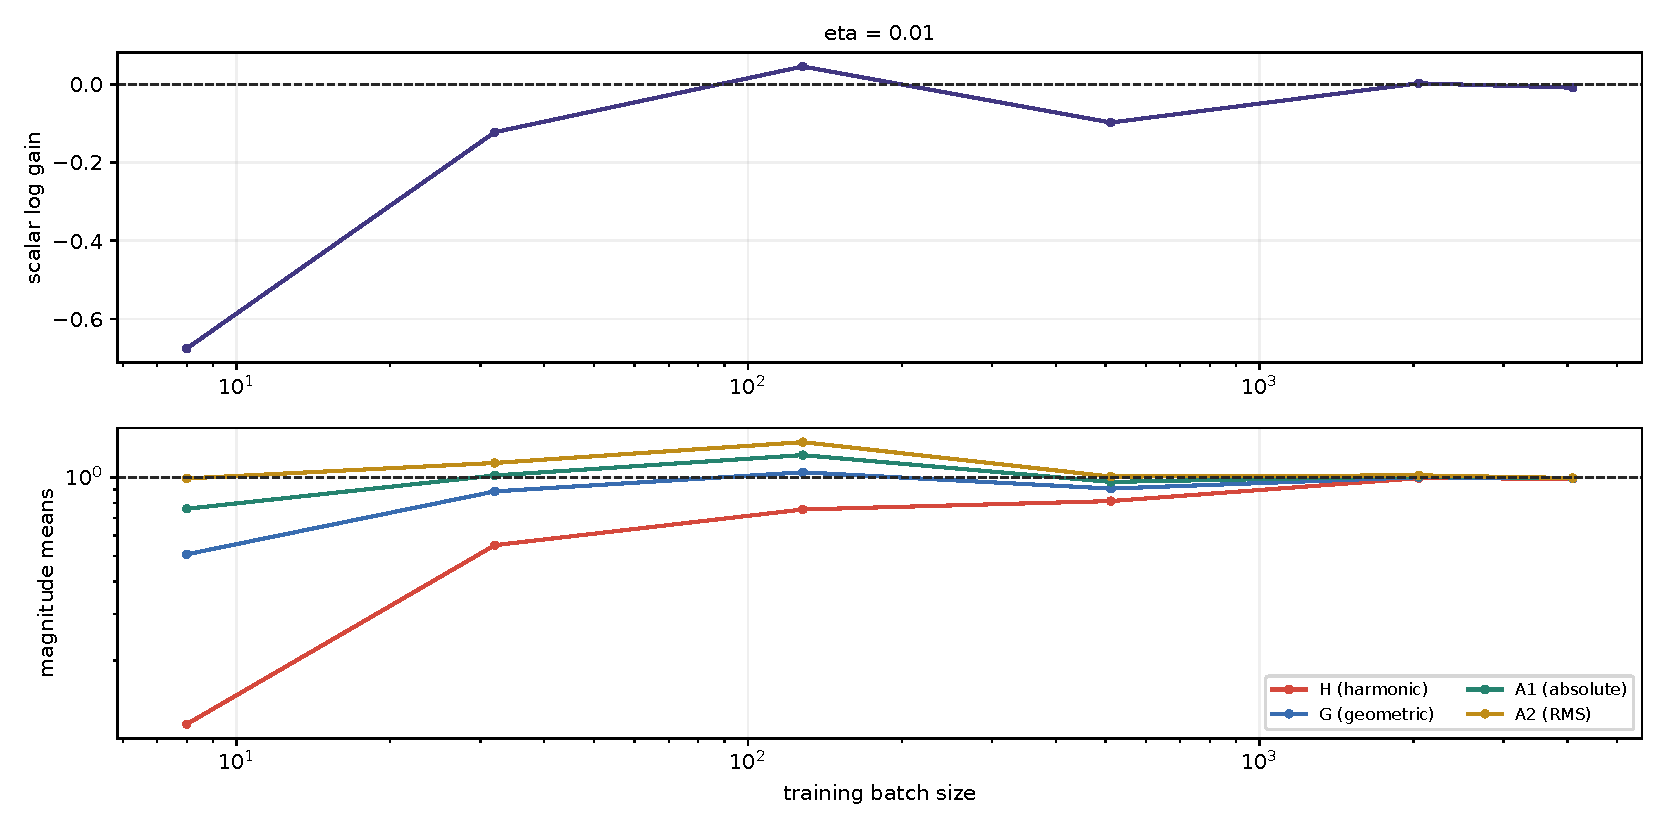
\includegraphics[width=\linewidth,height=0.78\textheight,keepaspectratio]{img/current_results/mlp_d3_02_moments.pdf}
\caption{\textbf{MLP, 3 x 256 (ReLU) | the moment ladder.} eta=0.01: step 39,999. Curves show average run-level measurements. H=1/E[1/|a|], G=exp(Lambda), A1=E|a|, A2=sqrt(E|a|\textasciicircum{}2). The lower panel uses a logarithmic scale. A mean of run-level H estimates is not H of a pooled distribution; finite estimates do not prove inverse-moment existence.}
\label{fig:current-mlp-d3-02-moments}
\end{figure}\clearpage

\begin{figure}[p]\centering
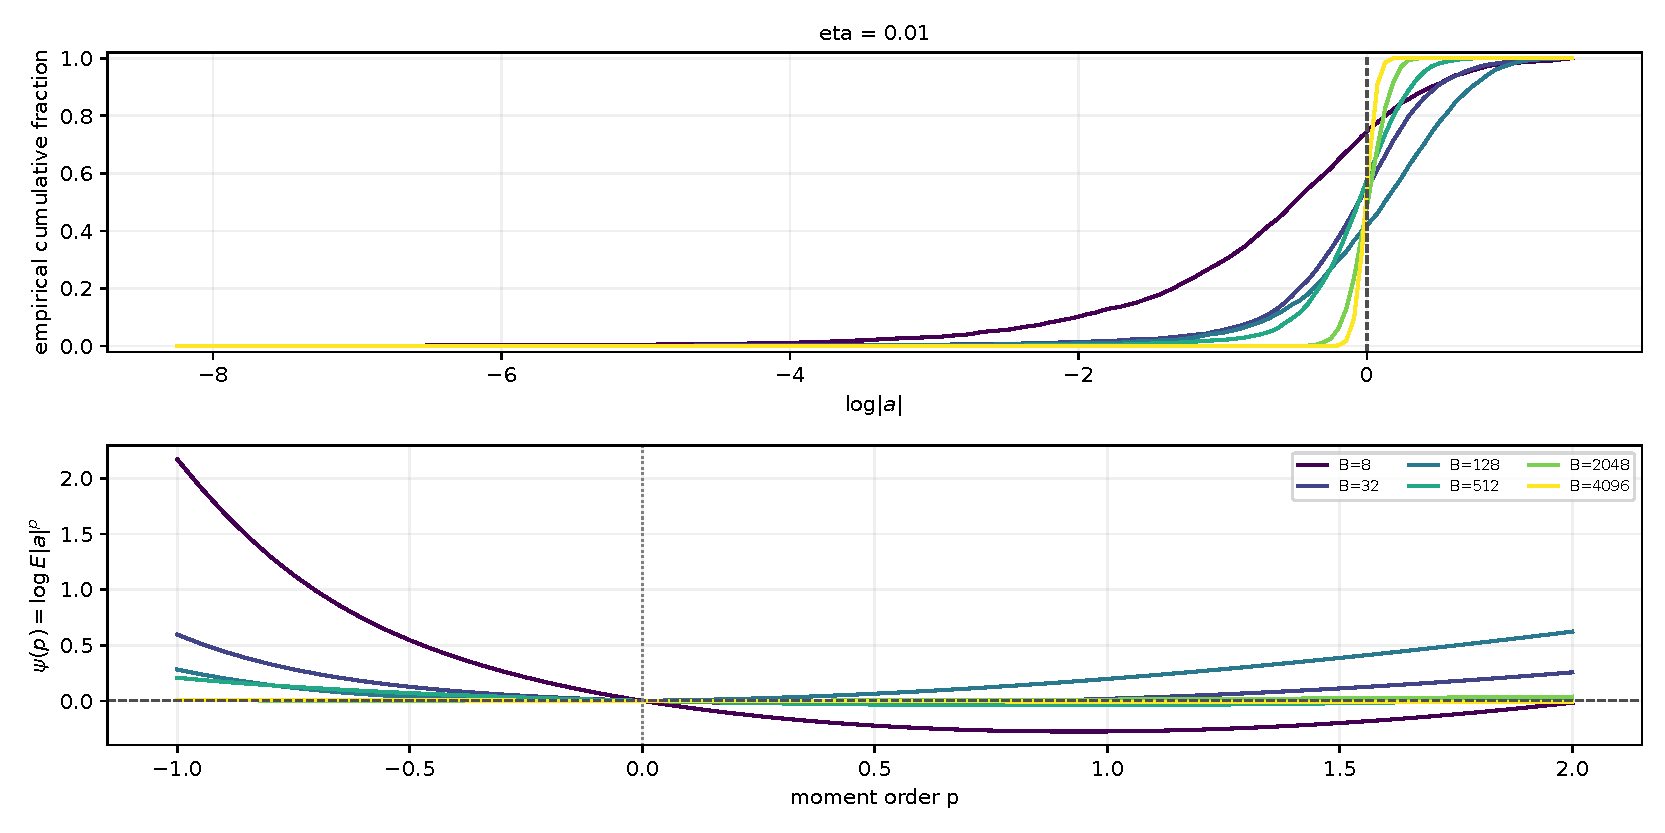
\includegraphics[width=\linewidth,height=0.78\textheight,keepaspectratio]{img/current_results/mlp_d3_03_gain_law.pdf}
\caption{\textbf{MLP, 3 x 256 (ReLU) | gain distributions and moment pressure.} eta=0.01: step 39,999. Curves show average run-level measurements. CDFs and log moments are computed within each run, then averaged equally. These are distributions of a conditional scalar multiplier, not distributions of a fixed parameter coordinate. Values near a=0 dominate inverse moments; p=0 is exactly zero by definition.}
\label{fig:current-mlp-d3-03-gain-law}
\end{figure}\clearpage

\begin{figure}[p]\centering
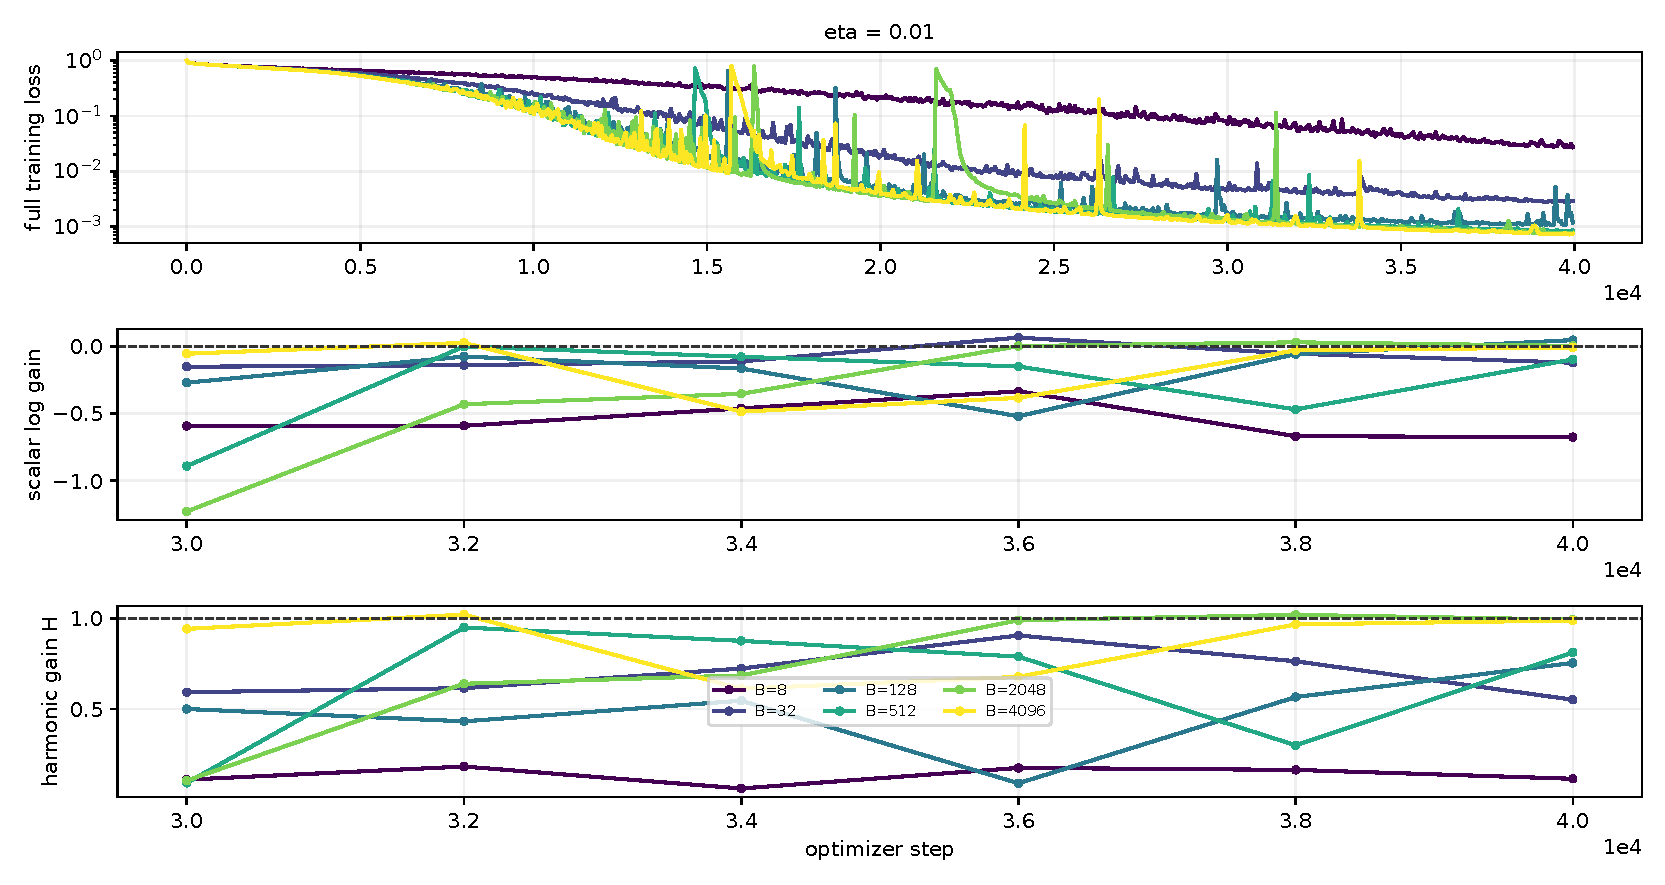
\includegraphics[width=\linewidth,height=0.78\textheight,keepaspectratio]{img/current_results/mlp_d3_04_dynamics.pdf}
\caption{\textbf{MLP, 3 x 256 (ReLU) | training and conditional gain dynamics.} Each batch curve averages run-level measurements at shared checkpoints and stops at the last common measurement. Loss and gain panels use their own recorded sampling grids. Finite training prefixes and decreasing loss do not establish a stationary distribution.}
\label{fig:current-mlp-d3-04-dynamics}
\end{figure}\clearpage

\begin{figure}[p]\centering
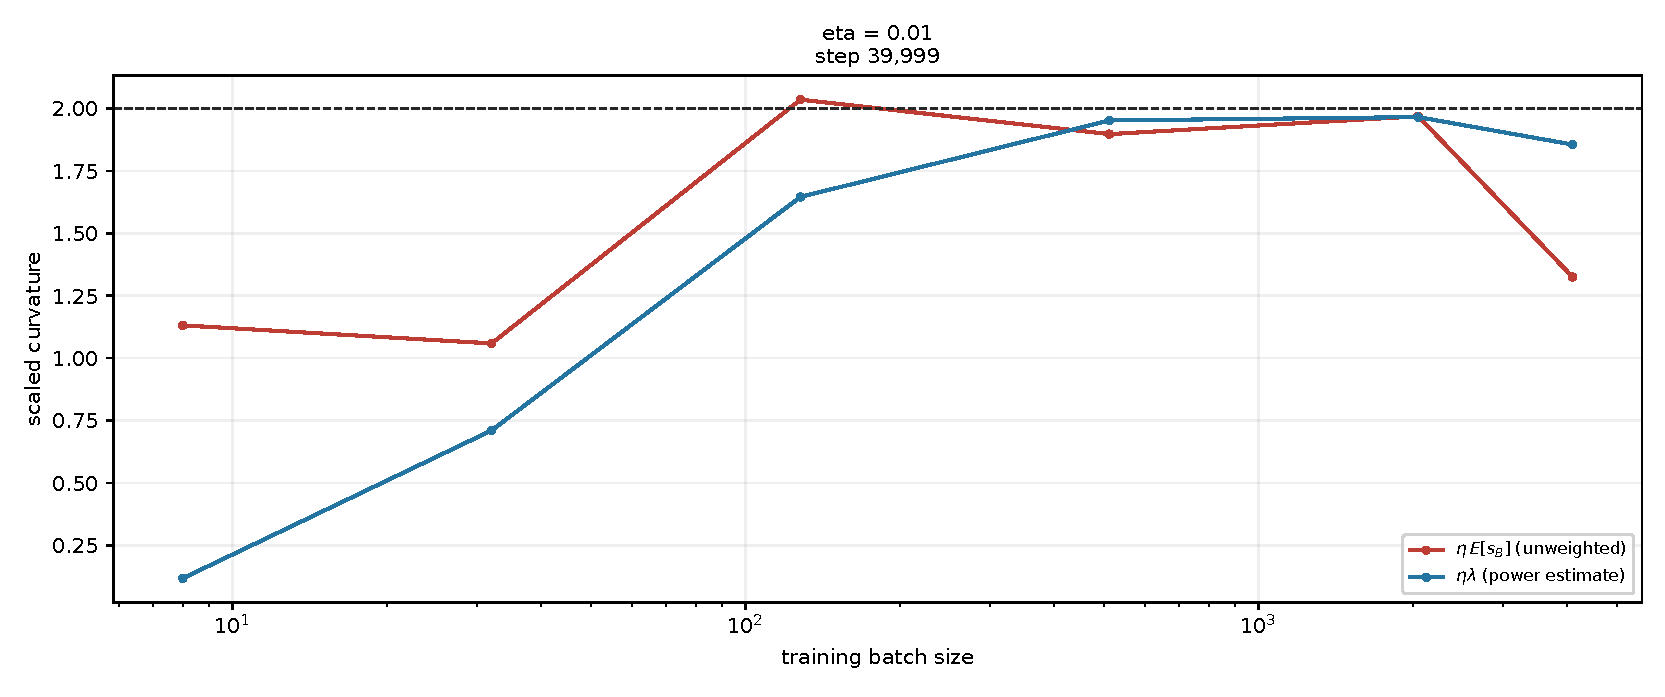
\includegraphics[width=\linewidth,height=0.78\textheight,keepaspectratio]{img/current_results/mlp_d4_01_curvature.pdf}
\caption{\textbf{MLP, 4 x 512 (ReLU) | curvature thresholds.} eta=0.01: step 39,999. Curves show average run-level measurements. The Hessian curve is a finite power-iteration estimate; it is not a certified largest eigenvalue. Actual saved learning rates are used. A red cross retains a pre-escape checkpoint.}
\label{fig:current-mlp-d4-01-curvature}
\end{figure}\clearpage

\begin{figure}[p]\centering
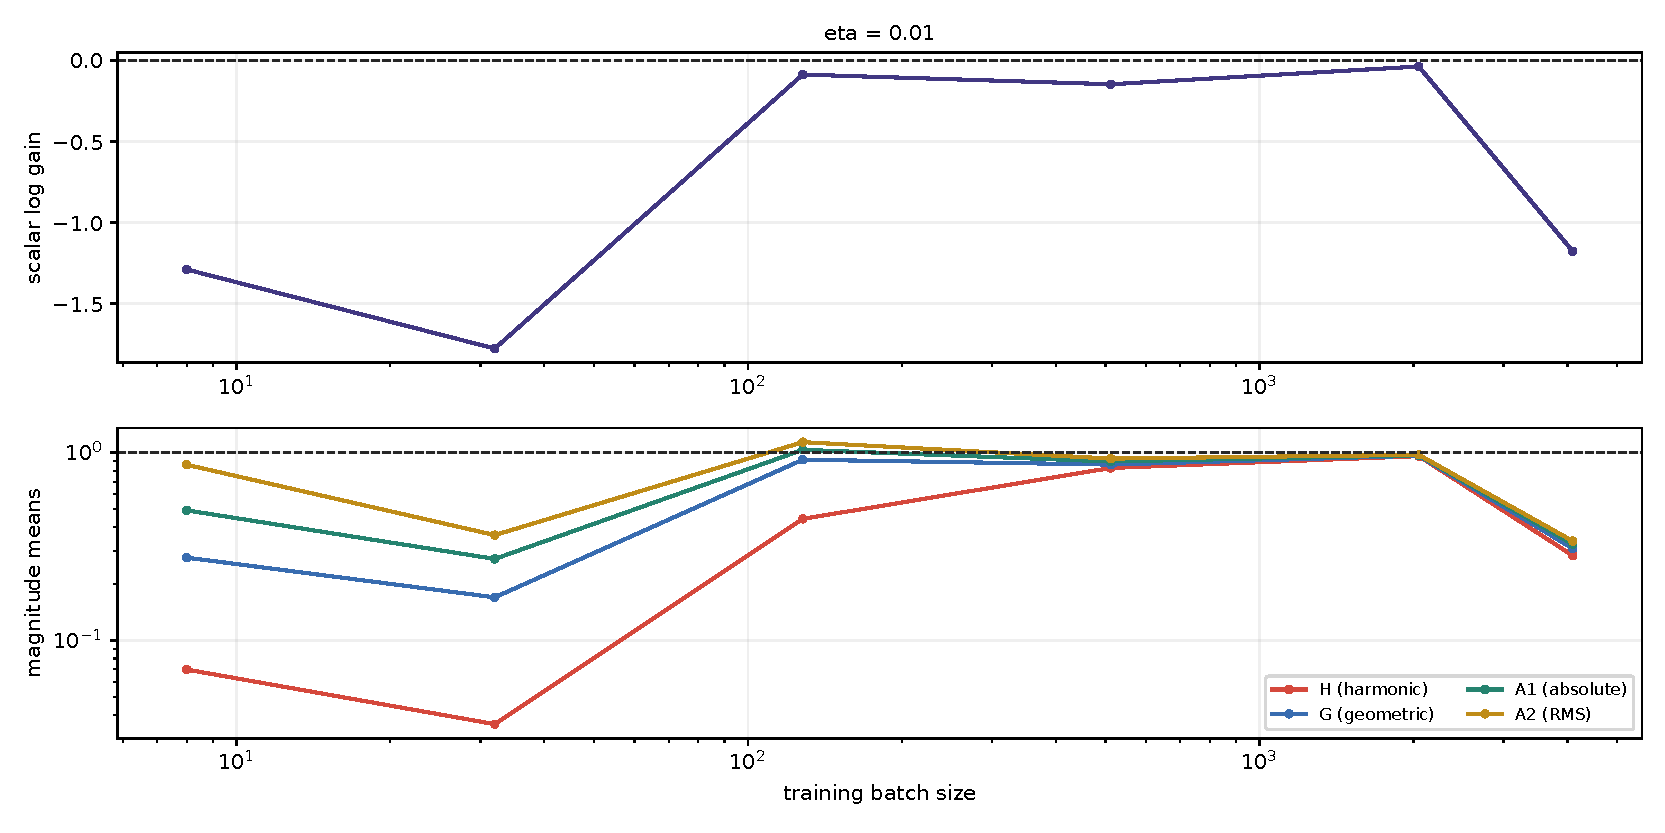
\includegraphics[width=\linewidth,height=0.78\textheight,keepaspectratio]{img/current_results/mlp_d4_02_moments.pdf}
\caption{\textbf{MLP, 4 x 512 (ReLU) | the moment ladder.} eta=0.01: step 39,999. Curves show average run-level measurements. H=1/E[1/|a|], G=exp(Lambda), A1=E|a|, A2=sqrt(E|a|\textasciicircum{}2). The lower panel uses a logarithmic scale. A mean of run-level H estimates is not H of a pooled distribution; finite estimates do not prove inverse-moment existence.}
\label{fig:current-mlp-d4-02-moments}
\end{figure}\clearpage

\begin{figure}[p]\centering
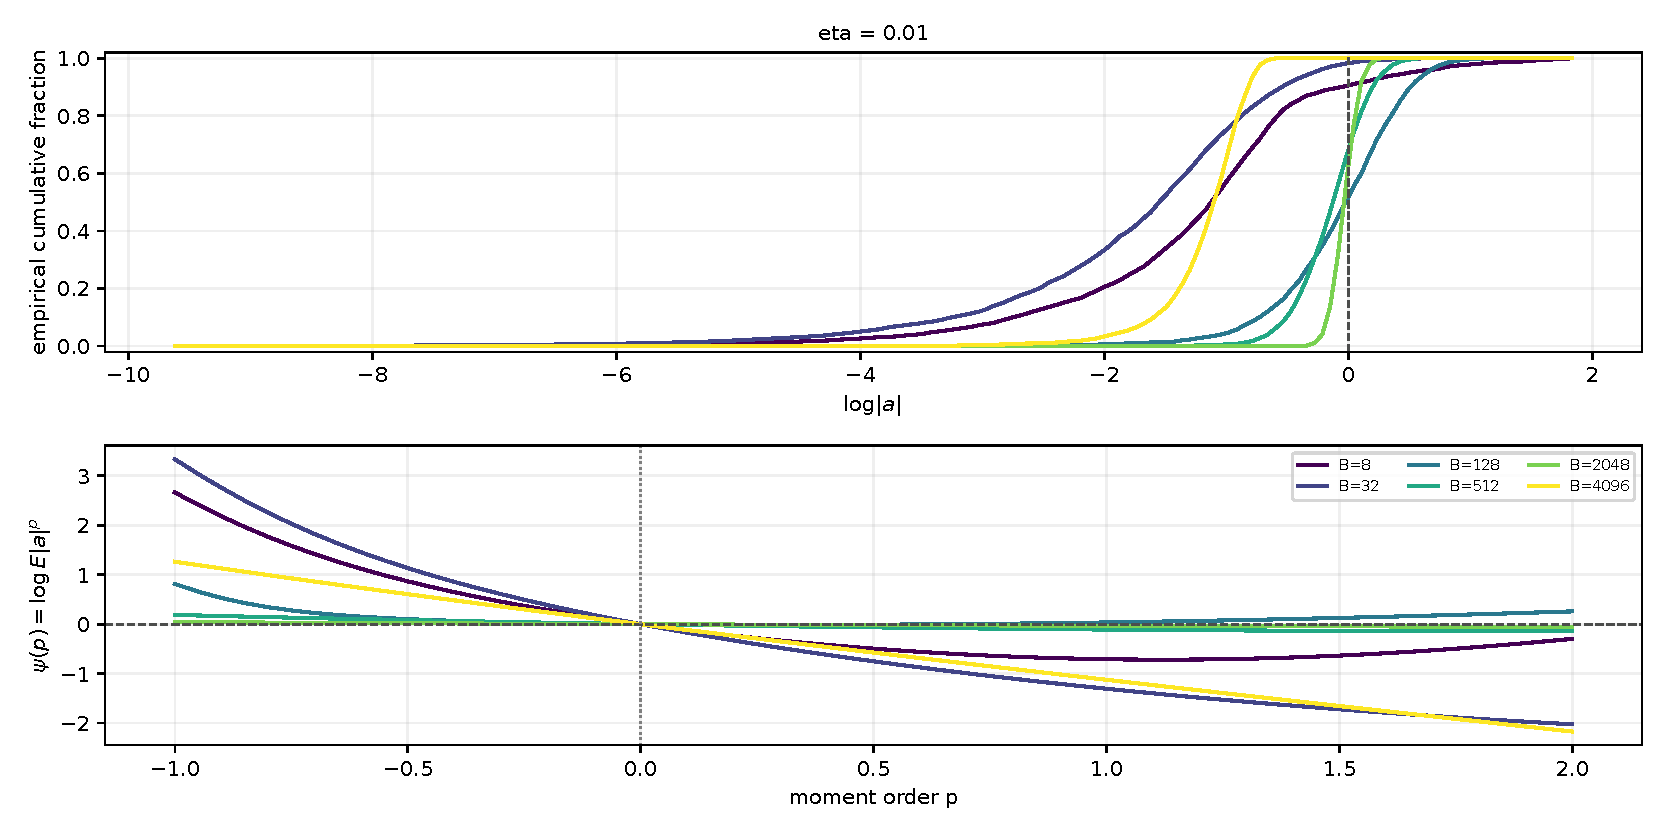
\includegraphics[width=\linewidth,height=0.78\textheight,keepaspectratio]{img/current_results/mlp_d4_03_gain_law.pdf}
\caption{\textbf{MLP, 4 x 512 (ReLU) | gain distributions and moment pressure.} eta=0.01: step 39,999. Curves show average run-level measurements. CDFs and log moments are computed within each run, then averaged equally. These are distributions of a conditional scalar multiplier, not distributions of a fixed parameter coordinate. Values near a=0 dominate inverse moments; p=0 is exactly zero by definition.}
\label{fig:current-mlp-d4-03-gain-law}
\end{figure}\clearpage

\begin{figure}[p]\centering
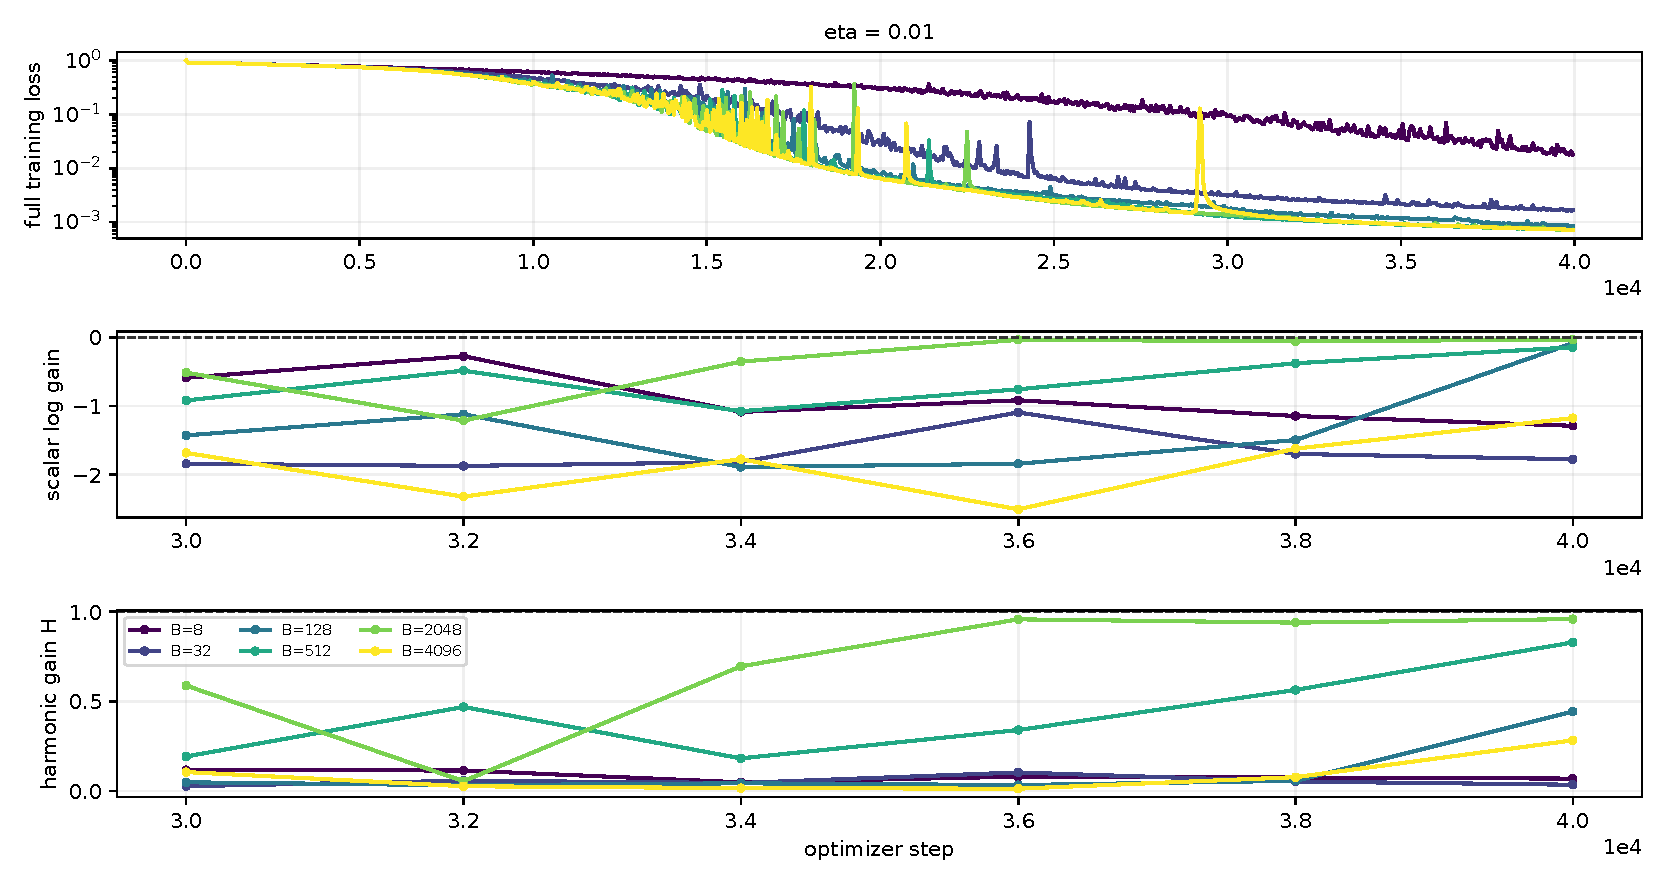
\includegraphics[width=\linewidth,height=0.78\textheight,keepaspectratio]{img/current_results/mlp_d4_04_dynamics.pdf}
\caption{\textbf{MLP, 4 x 512 (ReLU) | training and conditional gain dynamics.} Each batch curve averages run-level measurements at shared checkpoints and stops at the last common measurement. Loss and gain panels use their own recorded sampling grids. Finite training prefixes and decreasing loss do not establish a stationary distribution.}
\label{fig:current-mlp-d4-04-dynamics}
\end{figure}\clearpage

\begin{figure}[p]\centering
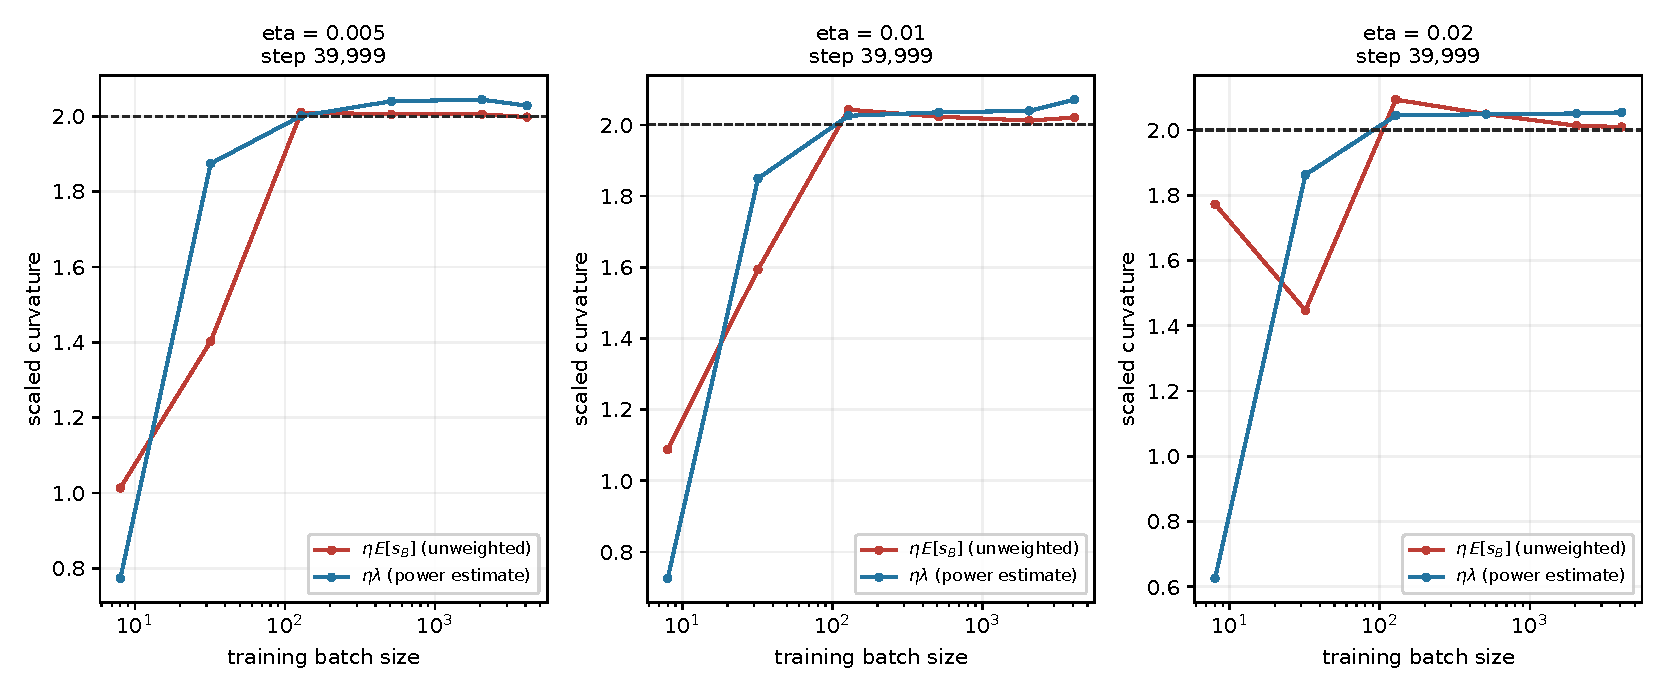
\includegraphics[width=\linewidth,height=0.78\textheight,keepaspectratio]{img/current_results/mlp_tanh_01_curvature.pdf}
\caption{\textbf{MLP, 2 x 512 (tanh) | curvature thresholds.} eta=0.005: step 39,999; eta=0.01: step 39,999; eta=0.02: step 39,999. Curves show average run-level measurements. The Hessian curve is a finite power-iteration estimate; it is not a certified largest eigenvalue. Actual saved learning rates are used. A red cross retains a pre-escape checkpoint.}
\label{fig:current-mlp-tanh-01-curvature}
\end{figure}\clearpage

\begin{figure}[p]\centering
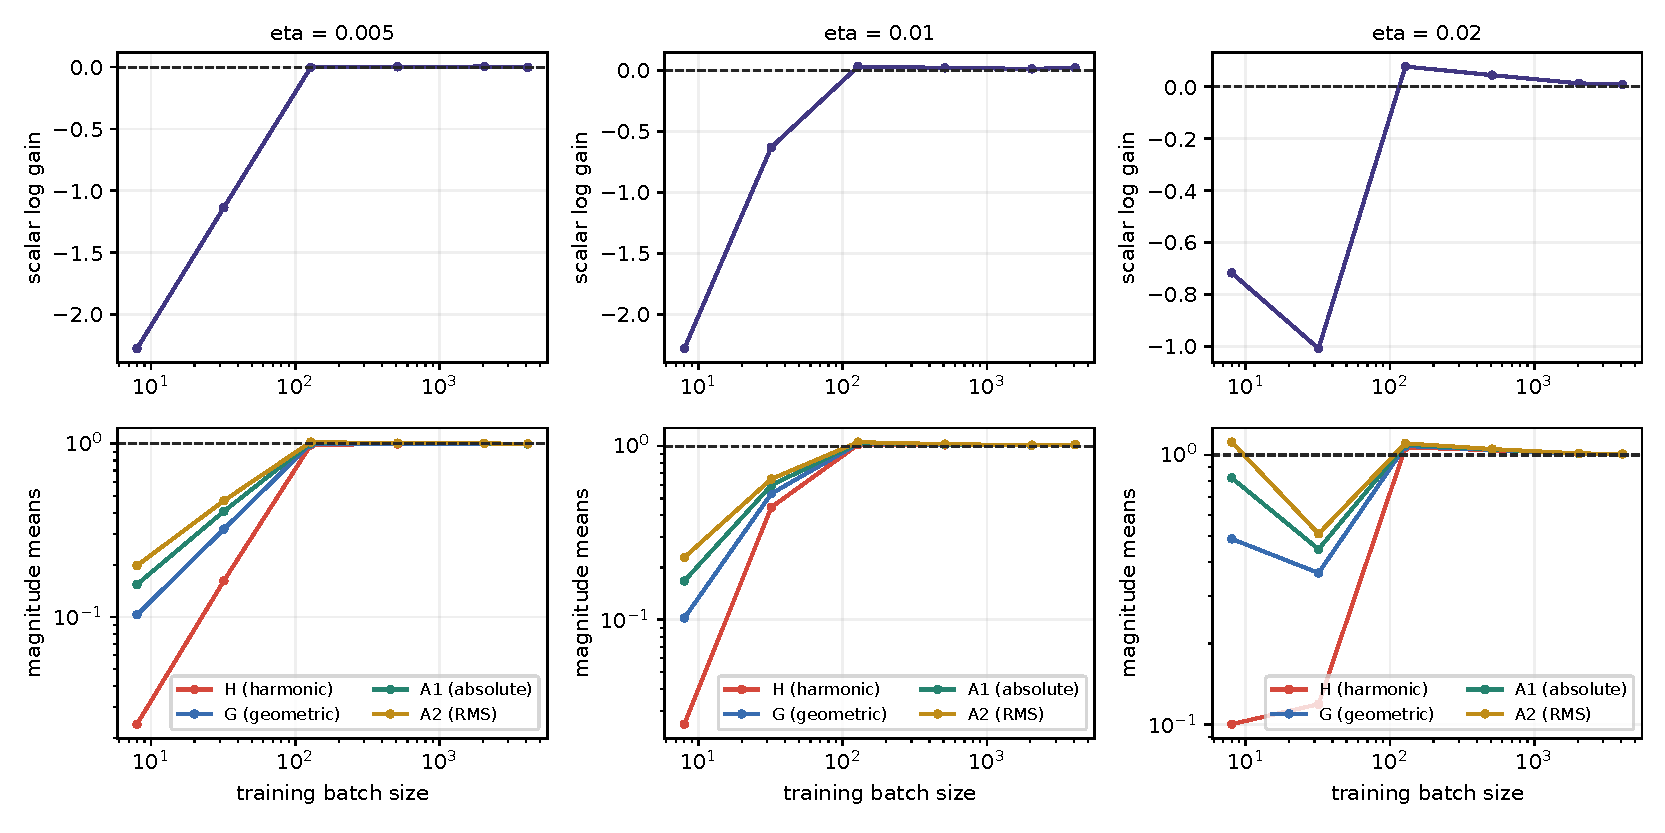
\includegraphics[width=\linewidth,height=0.78\textheight,keepaspectratio]{img/current_results/mlp_tanh_02_moments.pdf}
\caption{\textbf{MLP, 2 x 512 (tanh) | the moment ladder.} eta=0.005: step 39,999; eta=0.01: step 39,999; eta=0.02: step 39,999. Curves show average run-level measurements. H=1/E[1/|a|], G=exp(Lambda), A1=E|a|, A2=sqrt(E|a|\textasciicircum{}2). The lower panel uses a logarithmic scale. A mean of run-level H estimates is not H of a pooled distribution; finite estimates do not prove inverse-moment existence.}
\label{fig:current-mlp-tanh-02-moments}
\end{figure}\clearpage

\begin{figure}[p]\centering
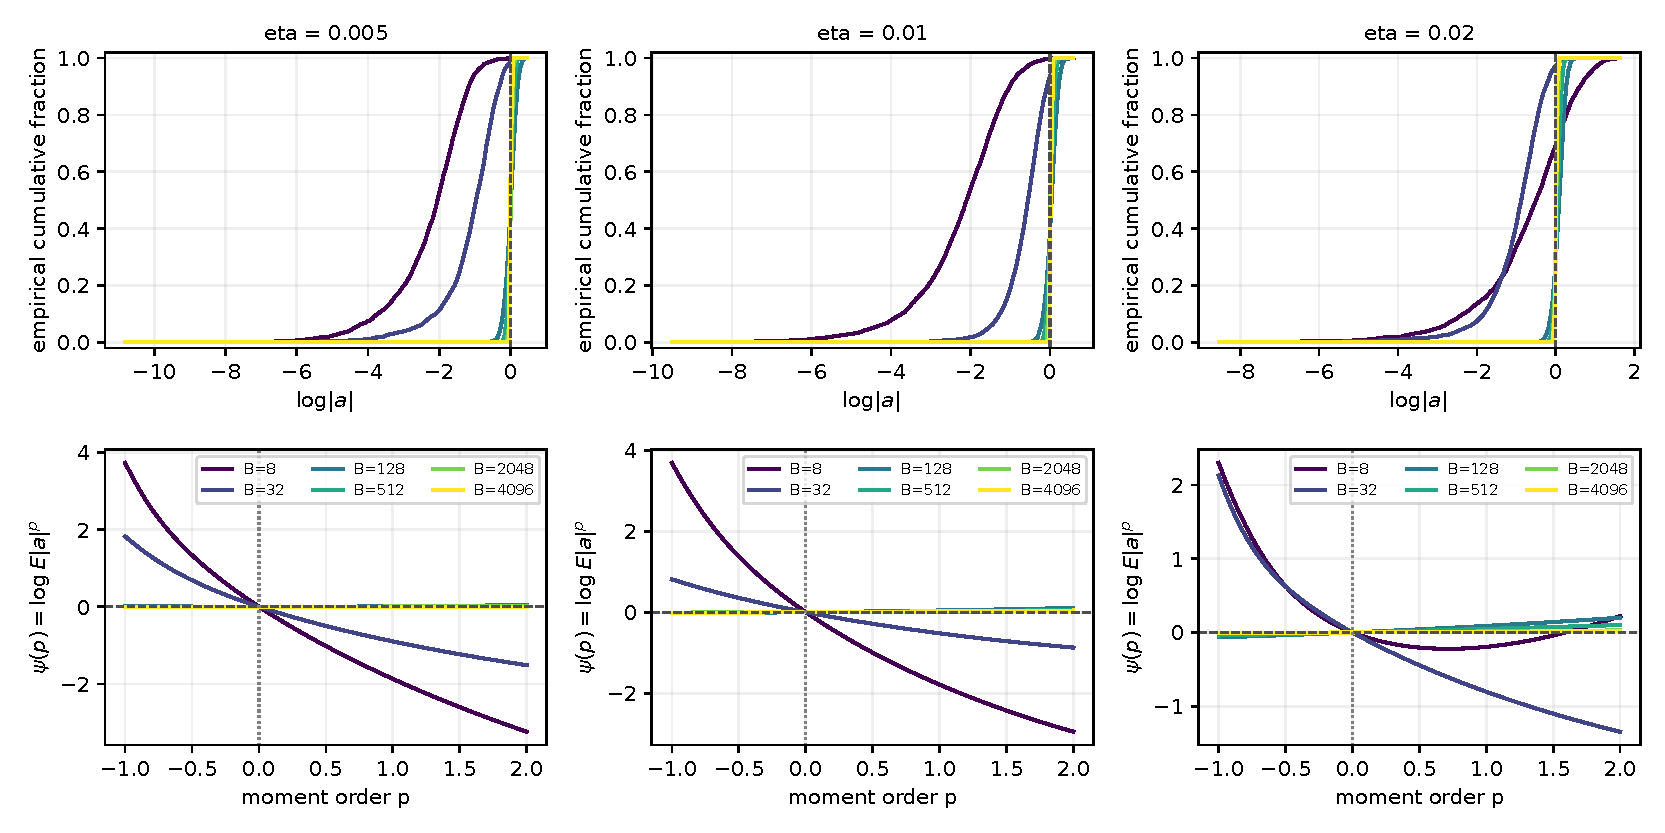
\includegraphics[width=\linewidth,height=0.78\textheight,keepaspectratio]{img/current_results/mlp_tanh_03_gain_law.pdf}
\caption{\textbf{MLP, 2 x 512 (tanh) | gain distributions and moment pressure.} eta=0.005: step 39,999; eta=0.01: step 39,999; eta=0.02: step 39,999. Curves show average run-level measurements. CDFs and log moments are computed within each run, then averaged equally. These are distributions of a conditional scalar multiplier, not distributions of a fixed parameter coordinate. Values near a=0 dominate inverse moments; p=0 is exactly zero by definition.}
\label{fig:current-mlp-tanh-03-gain-law}
\end{figure}\clearpage

\begin{figure}[p]\centering
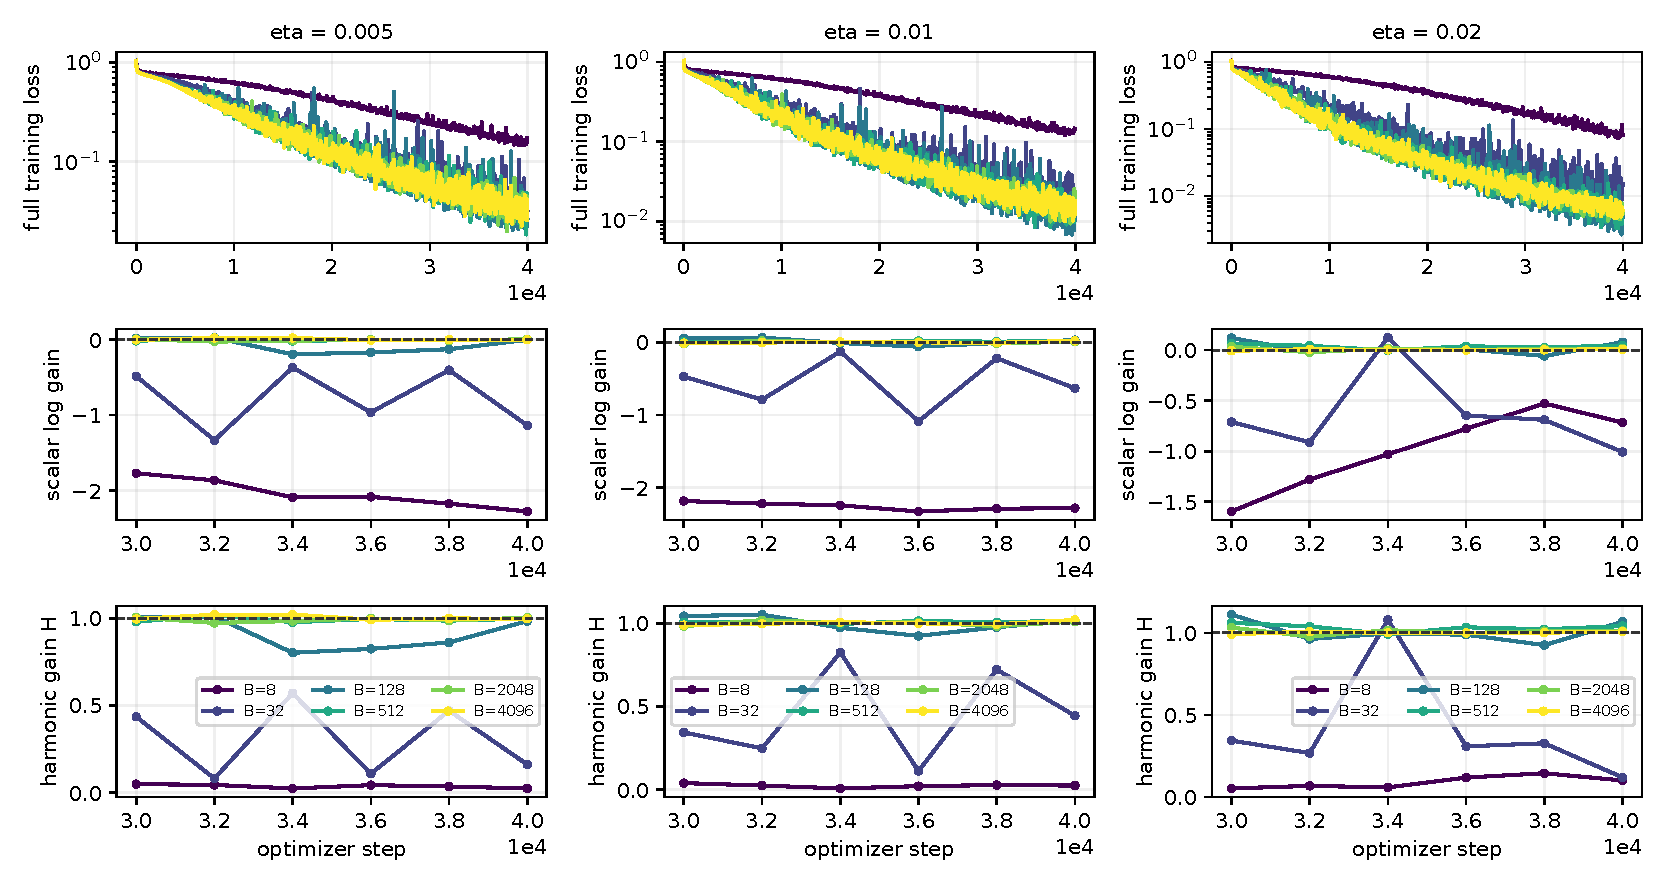
\includegraphics[width=\linewidth,height=0.78\textheight,keepaspectratio]{img/current_results/mlp_tanh_04_dynamics.pdf}
\caption{\textbf{MLP, 2 x 512 (tanh) | training and conditional gain dynamics.} Each batch curve averages run-level measurements at shared checkpoints and stops at the last common measurement. Loss and gain panels use their own recorded sampling grids. Finite training prefixes and decreasing loss do not establish a stationary distribution.}
\label{fig:current-mlp-tanh-04-dynamics}
\end{figure}\clearpage

\begin{figure}[p]\centering
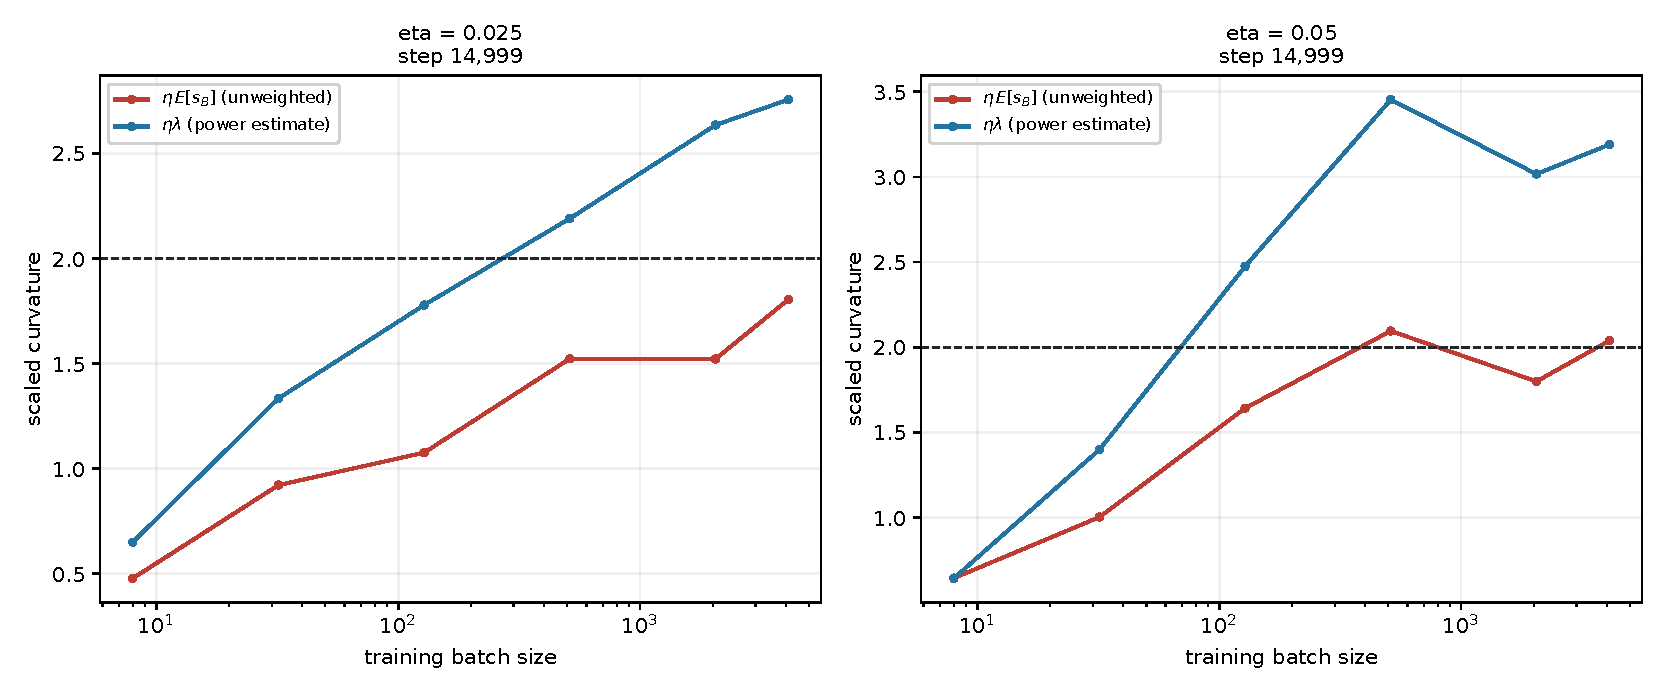
\includegraphics[width=\linewidth,height=0.78\textheight,keepaspectratio]{img/current_results/resnet20_01_curvature.pdf}
\caption{\textbf{ResNet-20 without BatchNorm | curvature thresholds.} eta=0.025: step 14,999; eta=0.05: step 14,999. Curves show average run-level measurements. The Hessian curve is a finite power-iteration estimate; it is not a certified largest eigenvalue. Actual saved learning rates are used. A red cross retains a pre-escape checkpoint.}
\label{fig:current-resnet20-01-curvature}
\end{figure}\clearpage

\begin{figure}[p]\centering
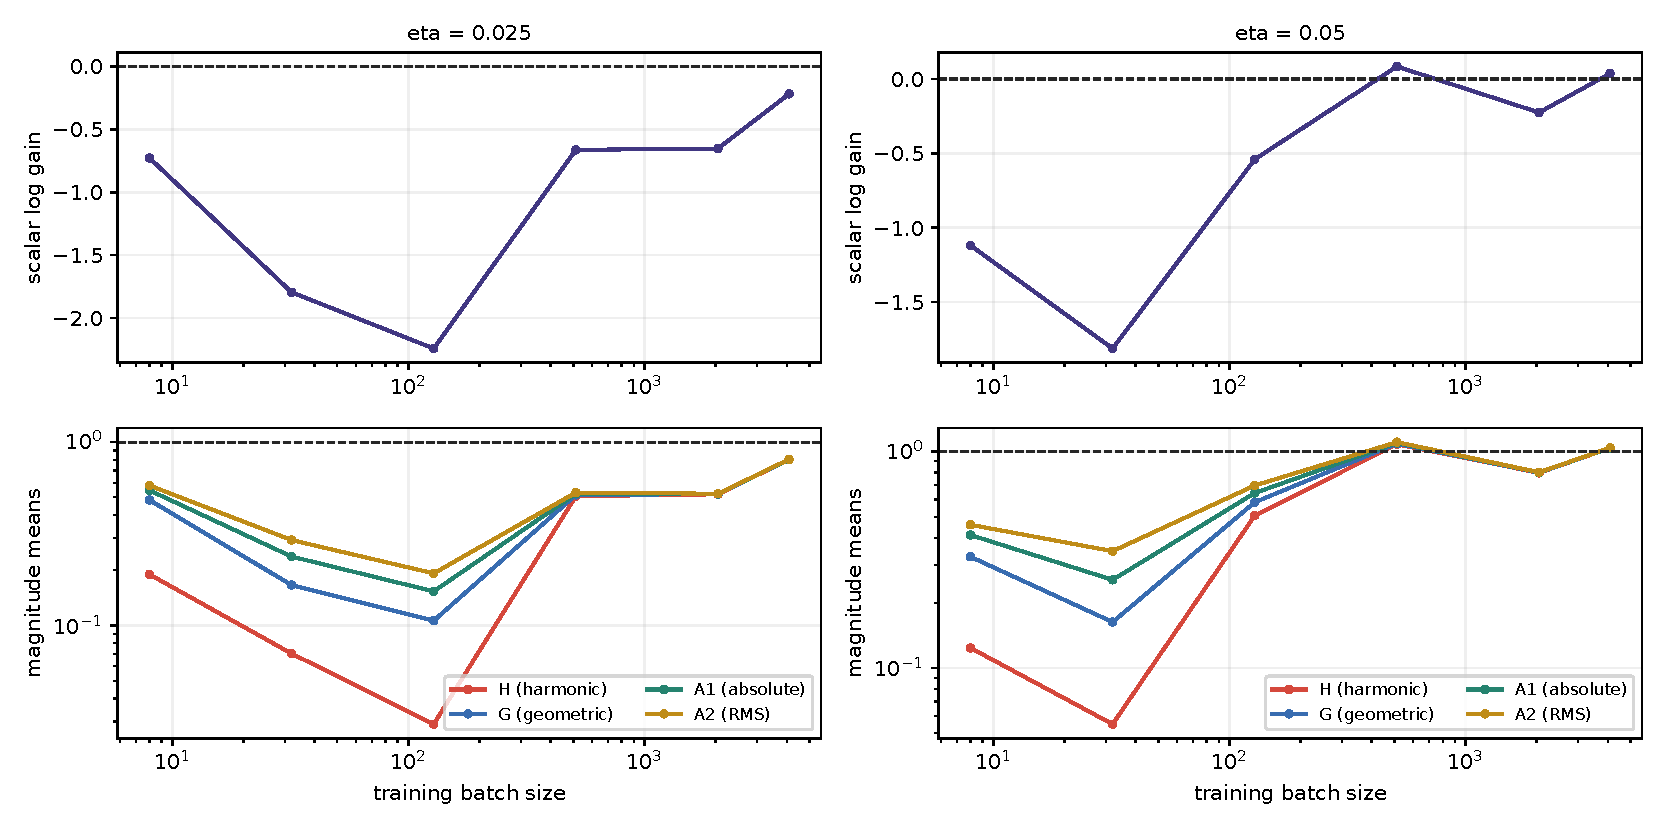
\includegraphics[width=\linewidth,height=0.78\textheight,keepaspectratio]{img/current_results/resnet20_02_moments.pdf}
\caption{\textbf{ResNet-20 without BatchNorm | the moment ladder.} eta=0.025: step 14,999; eta=0.05: step 14,999. Curves show average run-level measurements. H=1/E[1/|a|], G=exp(Lambda), A1=E|a|, A2=sqrt(E|a|\textasciicircum{}2). The lower panel uses a logarithmic scale. A mean of run-level H estimates is not H of a pooled distribution; finite estimates do not prove inverse-moment existence.}
\label{fig:current-resnet20-02-moments}
\end{figure}\clearpage

\begin{figure}[p]\centering
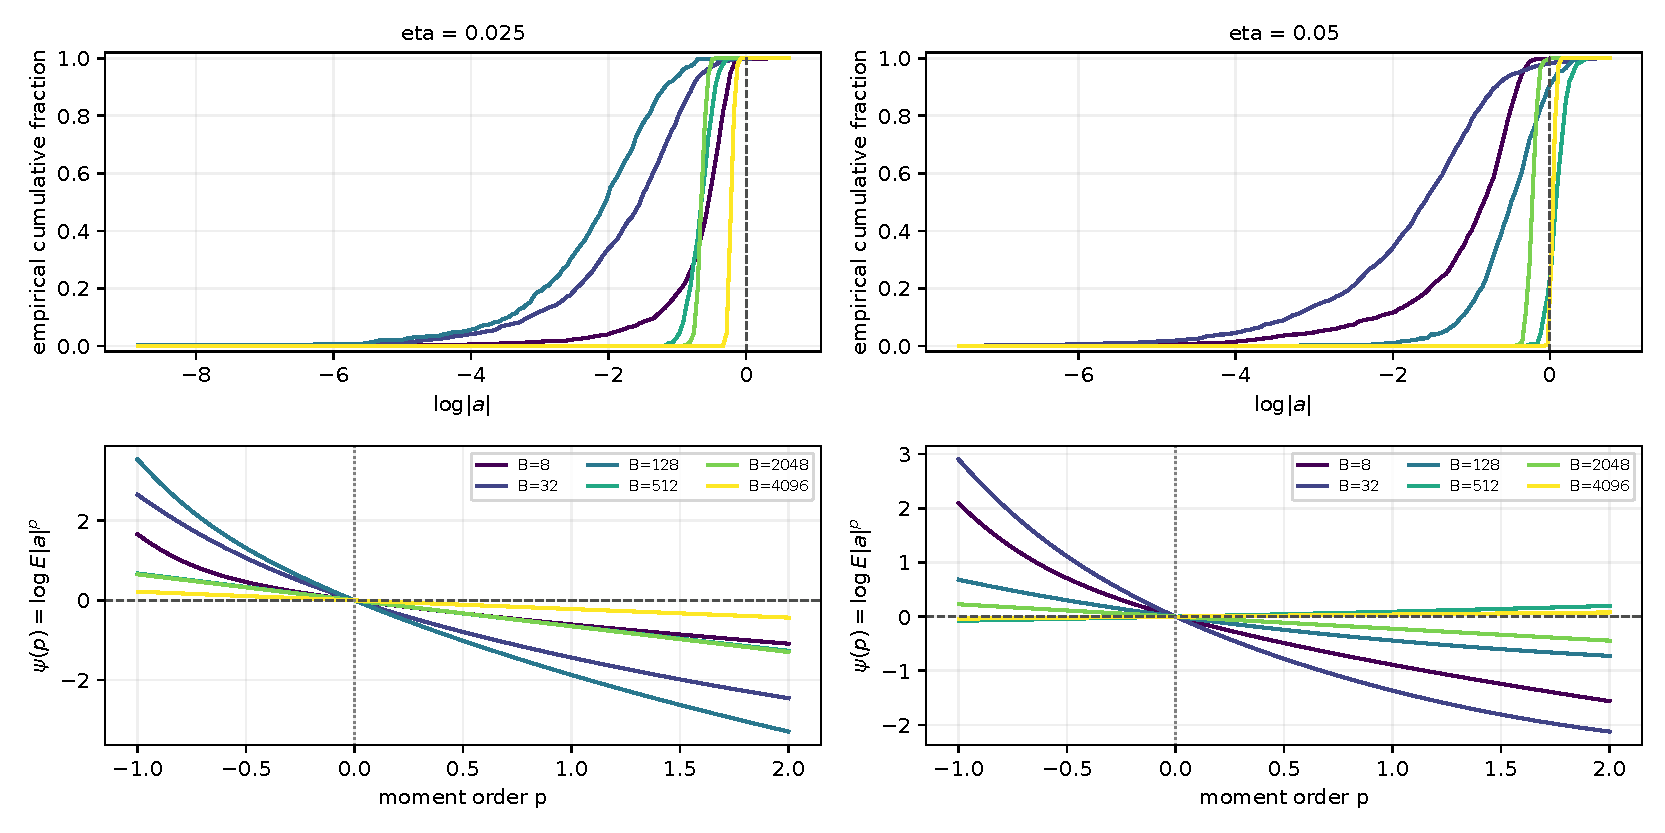
\includegraphics[width=\linewidth,height=0.78\textheight,keepaspectratio]{img/current_results/resnet20_03_gain_law.pdf}
\caption{\textbf{ResNet-20 without BatchNorm | gain distributions and moment pressure.} eta=0.025: step 14,999; eta=0.05: step 14,999. Curves show average run-level measurements. CDFs and log moments are computed within each run, then averaged equally. These are distributions of a conditional scalar multiplier, not distributions of a fixed parameter coordinate. Values near a=0 dominate inverse moments; p=0 is exactly zero by definition.}
\label{fig:current-resnet20-03-gain-law}
\end{figure}\clearpage

\begin{figure}[p]\centering
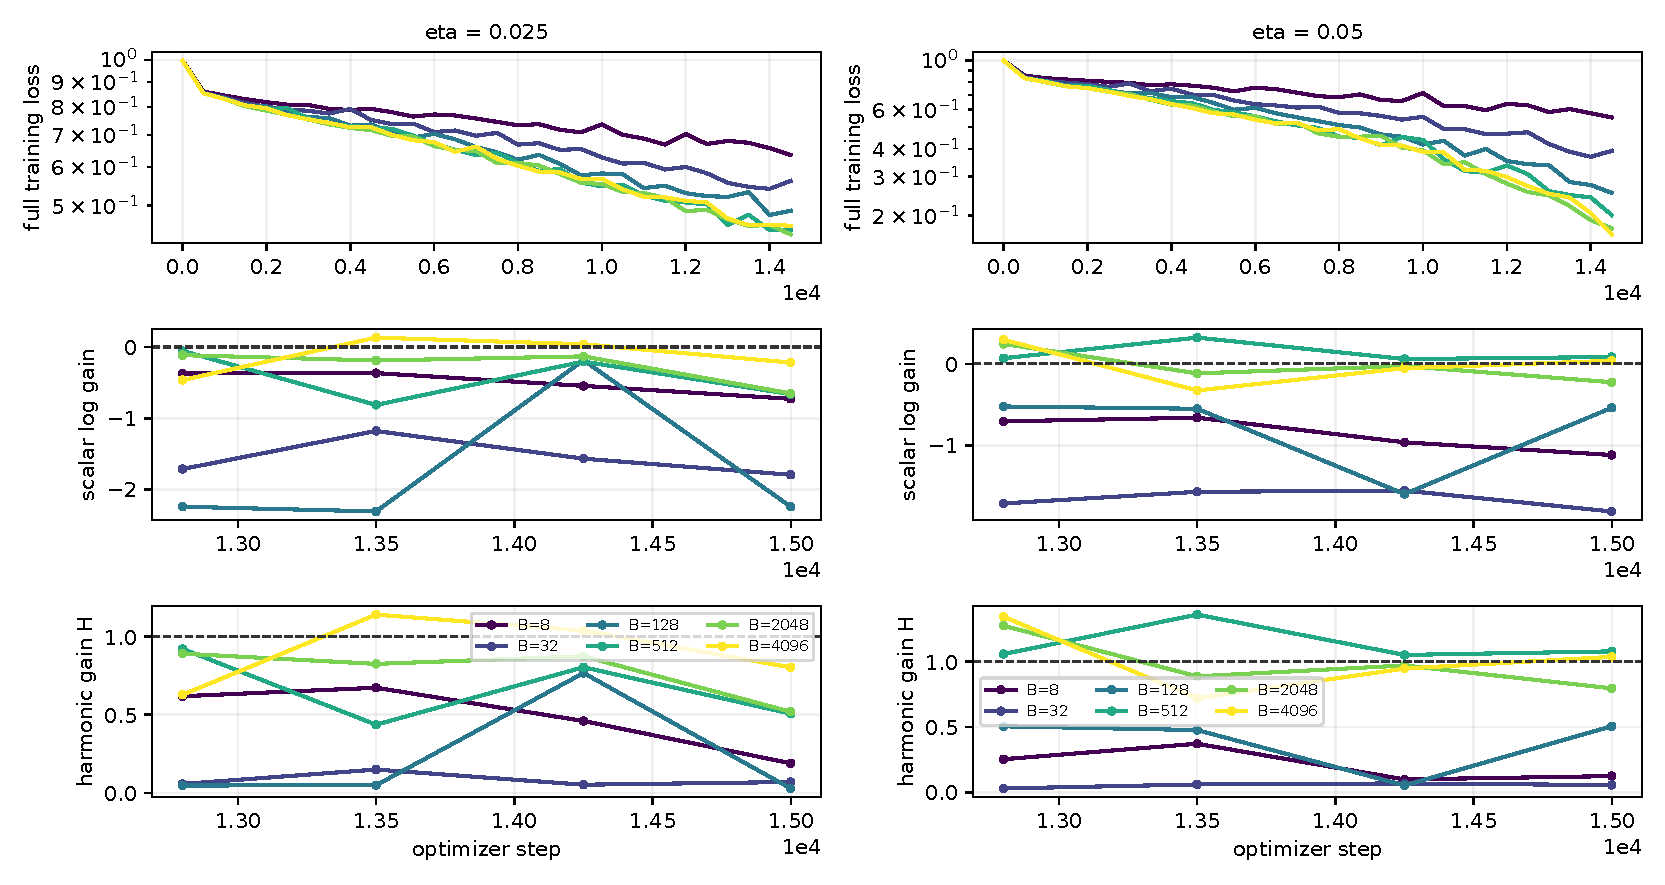
\includegraphics[width=\linewidth,height=0.78\textheight,keepaspectratio]{img/current_results/resnet20_04_dynamics.pdf}
\caption{\textbf{ResNet-20 without BatchNorm | training and conditional gain dynamics.} Each batch curve averages run-level measurements at shared checkpoints and stops at the last common measurement. Loss and gain panels use their own recorded sampling grids. Finite training prefixes and decreasing loss do not establish a stationary distribution.}
\label{fig:current-resnet20-04-dynamics}
\end{figure}\clearpage

\begin{figure}[p]\centering
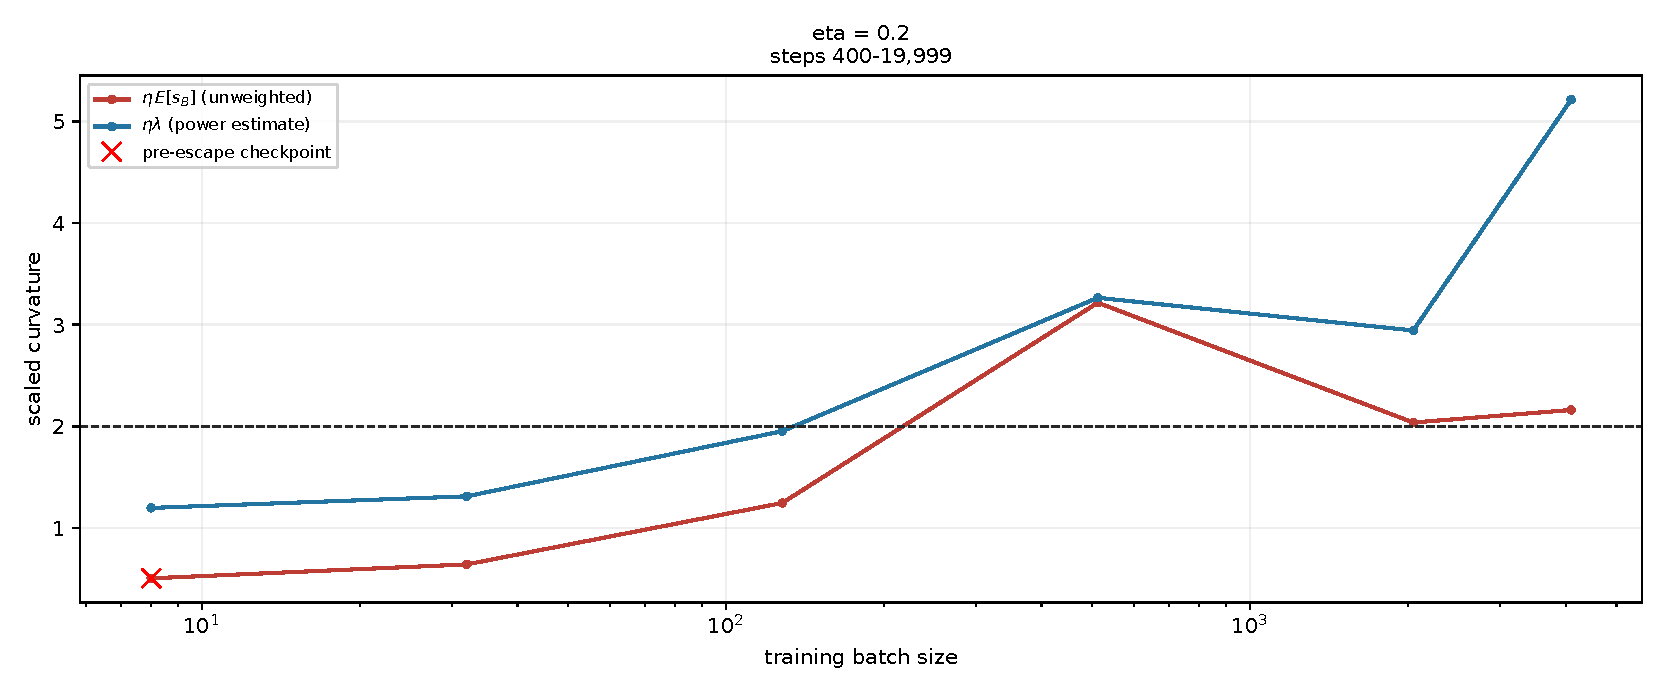
\includegraphics[width=\linewidth,height=0.78\textheight,keepaspectratio]{img/current_results/vit_01_curvature.pdf}
\caption{\textbf{ViT, 2 blocks x width 64 | curvature thresholds.} eta=0.2: steps 400-19,999. Curves show average run-level measurements. The Hessian curve is a finite power-iteration estimate; it is not a certified largest eigenvalue. Actual saved learning rates are used. A red cross retains a pre-escape checkpoint.}
\label{fig:current-vit-01-curvature}
\end{figure}\clearpage

\begin{figure}[p]\centering
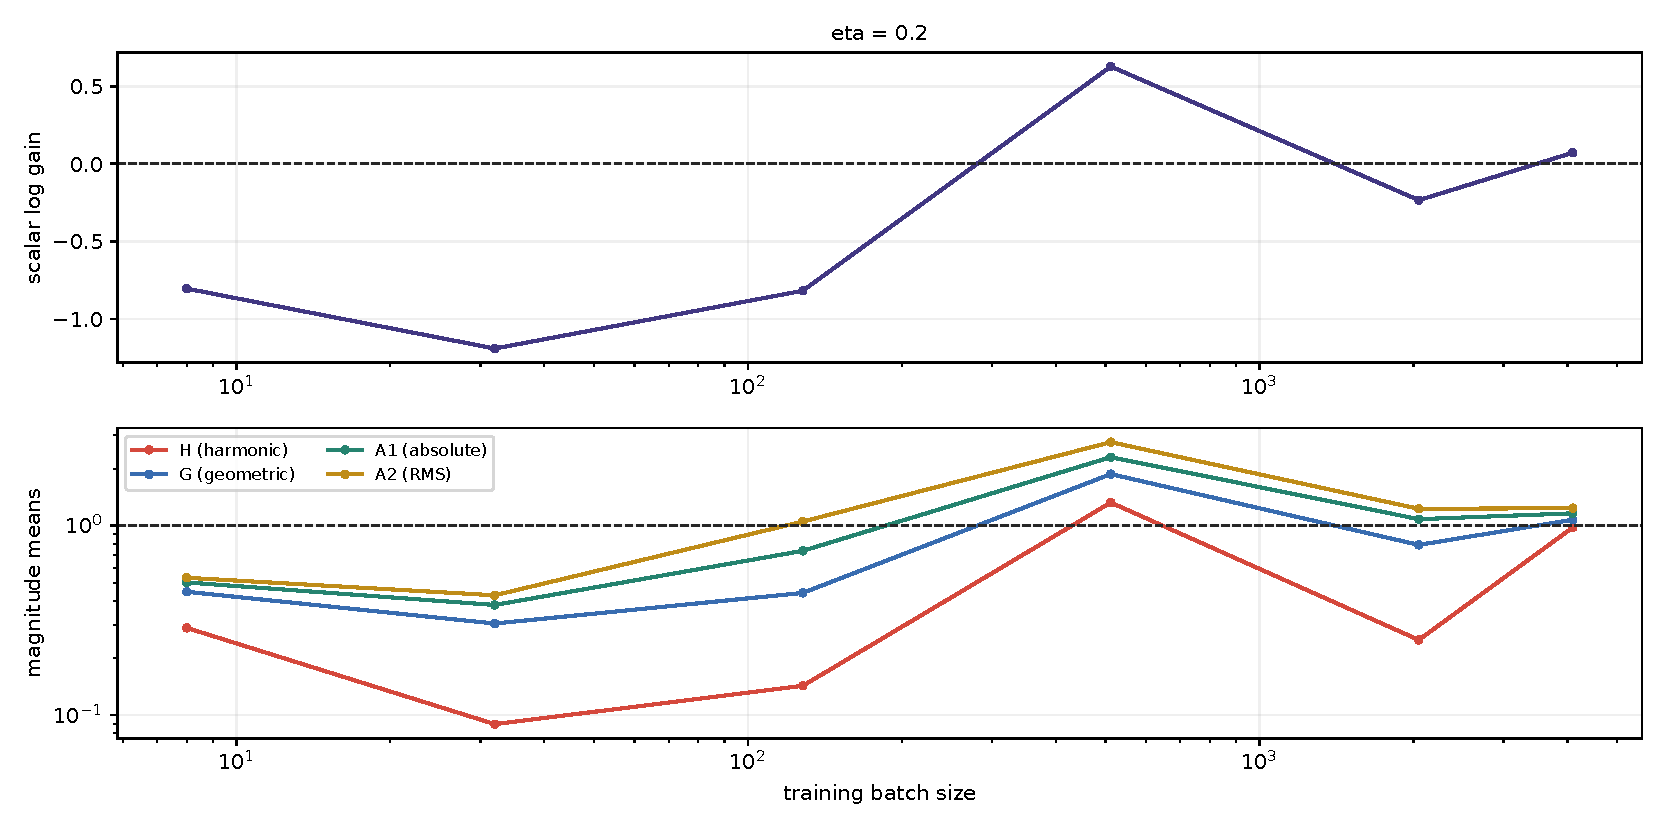
\includegraphics[width=\linewidth,height=0.78\textheight,keepaspectratio]{img/current_results/vit_02_moments.pdf}
\caption{\textbf{ViT, 2 blocks x width 64 | the moment ladder.} eta=0.2: steps 400-19,999. Curves show average run-level measurements. H=1/E[1/|a|], G=exp(Lambda), A1=E|a|, A2=sqrt(E|a|\textasciicircum{}2). The lower panel uses a logarithmic scale. A mean of run-level H estimates is not H of a pooled distribution; finite estimates do not prove inverse-moment existence.}
\label{fig:current-vit-02-moments}
\end{figure}\clearpage

\begin{figure}[p]\centering
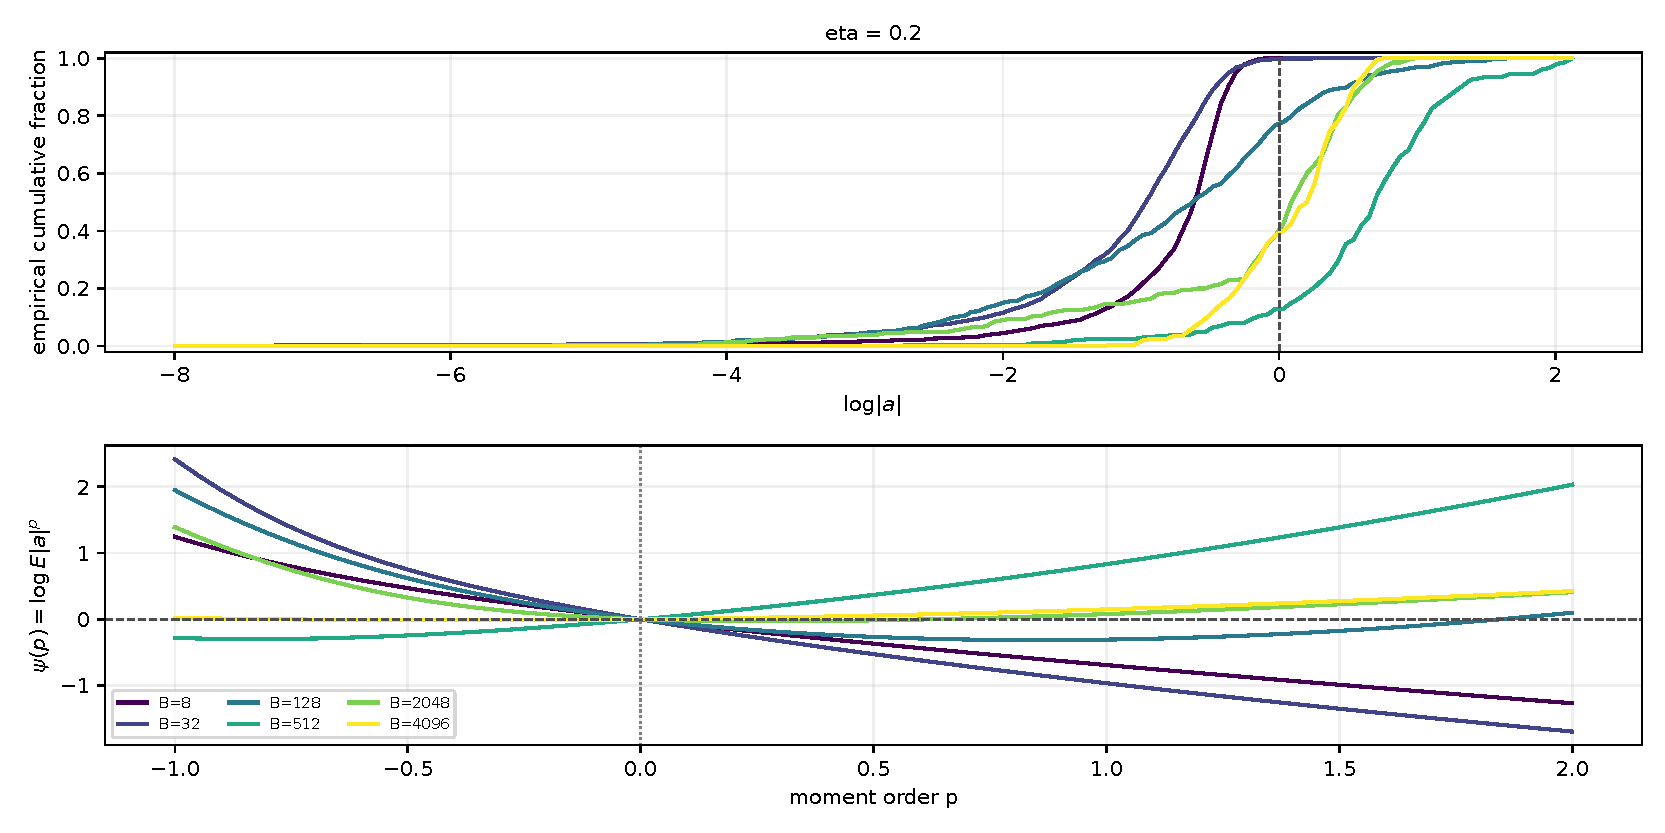
\includegraphics[width=\linewidth,height=0.78\textheight,keepaspectratio]{img/current_results/vit_03_gain_law.pdf}
\caption{\textbf{ViT, 2 blocks x width 64 | gain distributions and moment pressure.} eta=0.2: steps 400-19,999. Curves show average run-level measurements. CDFs and log moments are computed within each run, then averaged equally. These are distributions of a conditional scalar multiplier, not distributions of a fixed parameter coordinate. Values near a=0 dominate inverse moments; p=0 is exactly zero by definition.}
\label{fig:current-vit-03-gain-law}
\end{figure}\clearpage

\begin{figure}[p]\centering
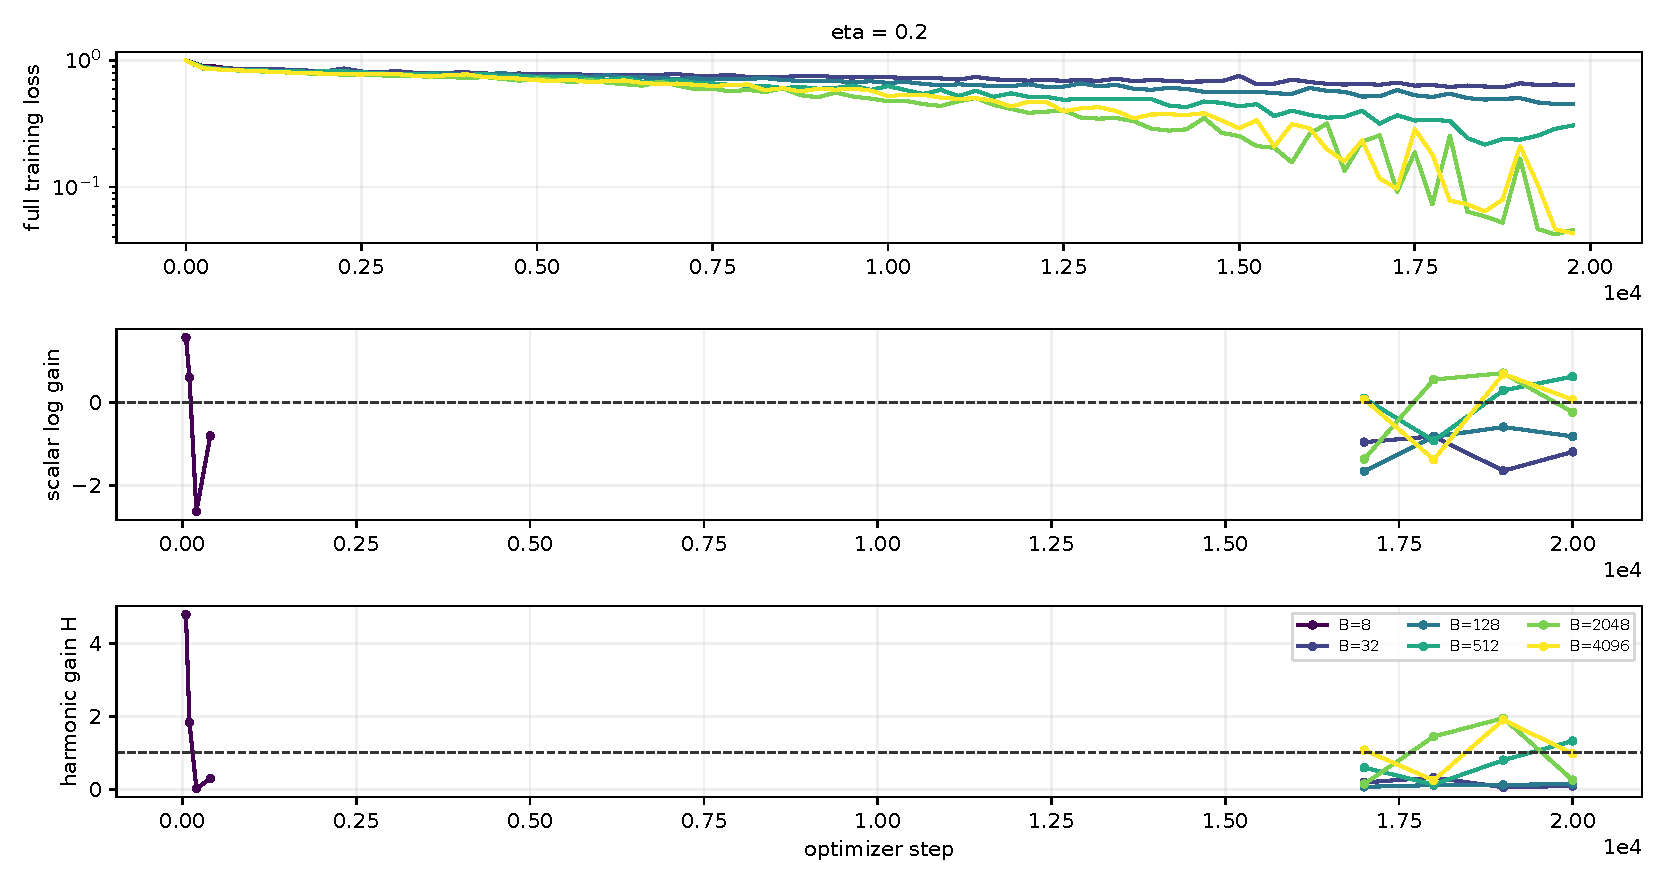
\includegraphics[width=\linewidth,height=0.78\textheight,keepaspectratio]{img/current_results/vit_04_dynamics.pdf}
\caption{\textbf{ViT, 2 blocks x width 64 | training and conditional gain dynamics.} Each batch curve averages run-level measurements at shared checkpoints and stops at the last common measurement. Loss and gain panels use their own recorded sampling grids. Finite training prefixes and decreasing loss do not establish a stationary distribution.}
\label{fig:current-vit-04-dynamics}
\end{figure}\clearpage

\begin{figure}[p]\centering
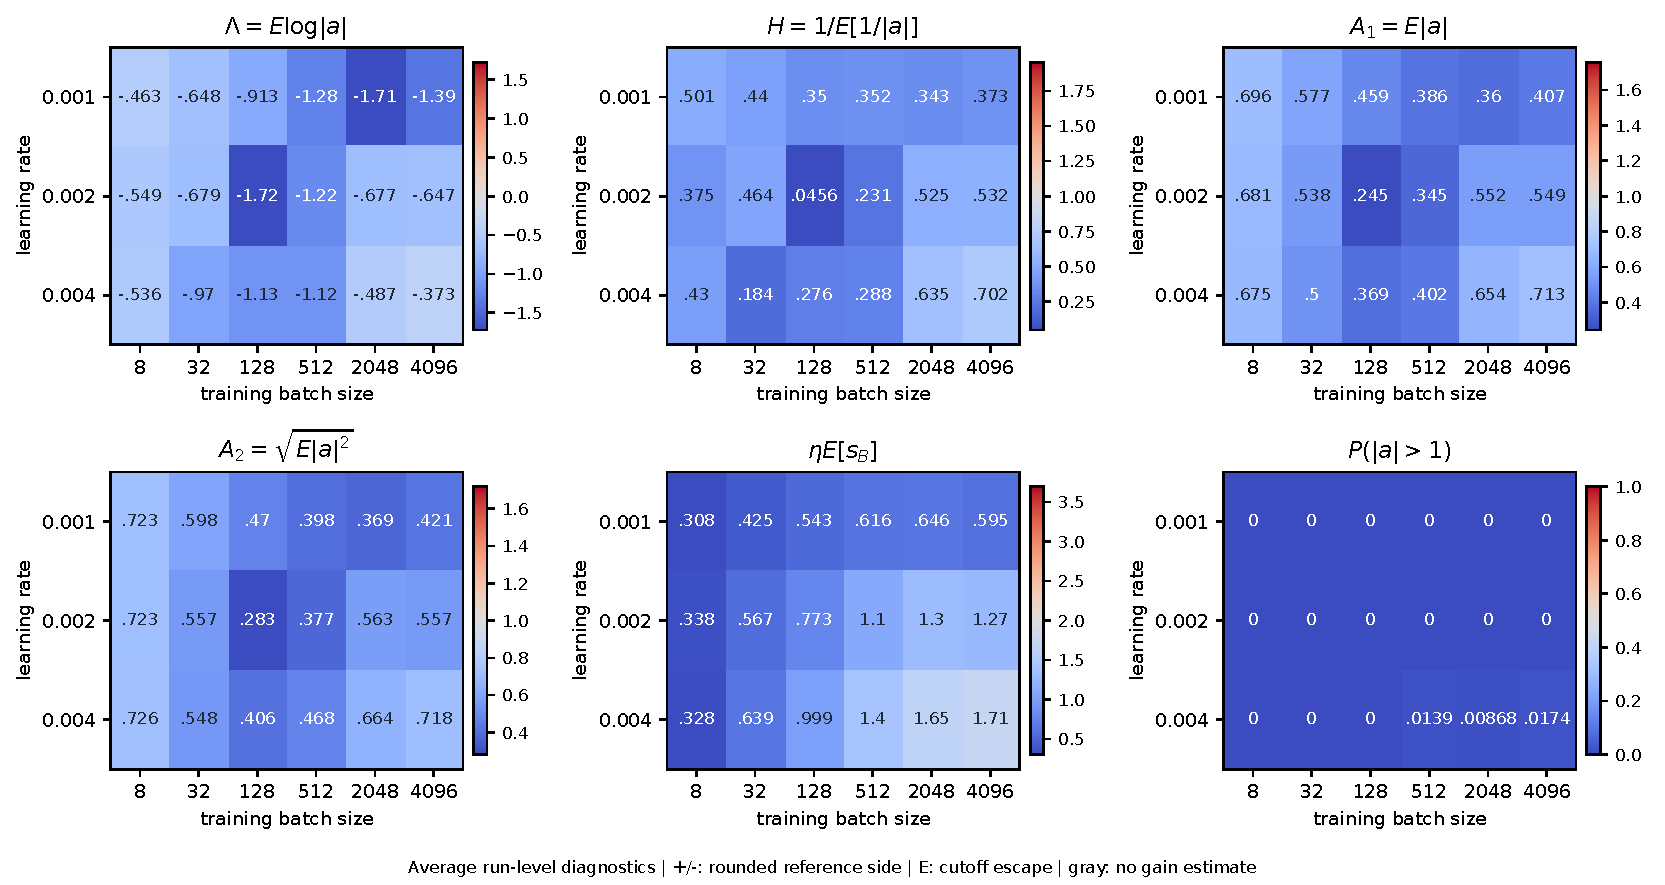
\includegraphics[width=\linewidth,height=0.78\textheight,keepaspectratio]{img/current_results/wrn_no_bn_grid_eta_batch.pdf}
\caption{\textbf{WideResNet-10-2, native Fixup | stability grid over batch size and step size.} Axes are actual training learning rate and batch size. The six panels show Lambda, H, A1, A2, eta E[s\_B], and the fraction of expanding gains. Each cell averages run-level statistics from the final three available checkpoints; time windows can differ across settings and runs. Color centers are 0, 1, 1, 1, 2, and 0.5. Curvature and expansion-fraction centers are references, not full-network stability tests. A trailing +/- preserves the side of a reference after rounding. Gray means no gain estimate; E marks a recorded escape, including pre-escape estimates. Finite H does not establish population inverse-moment finiteness.}
\label{fig:current-wrn-no-bn-grid-eta-batch}
\end{figure}\clearpage

\begin{figure}[p]\centering
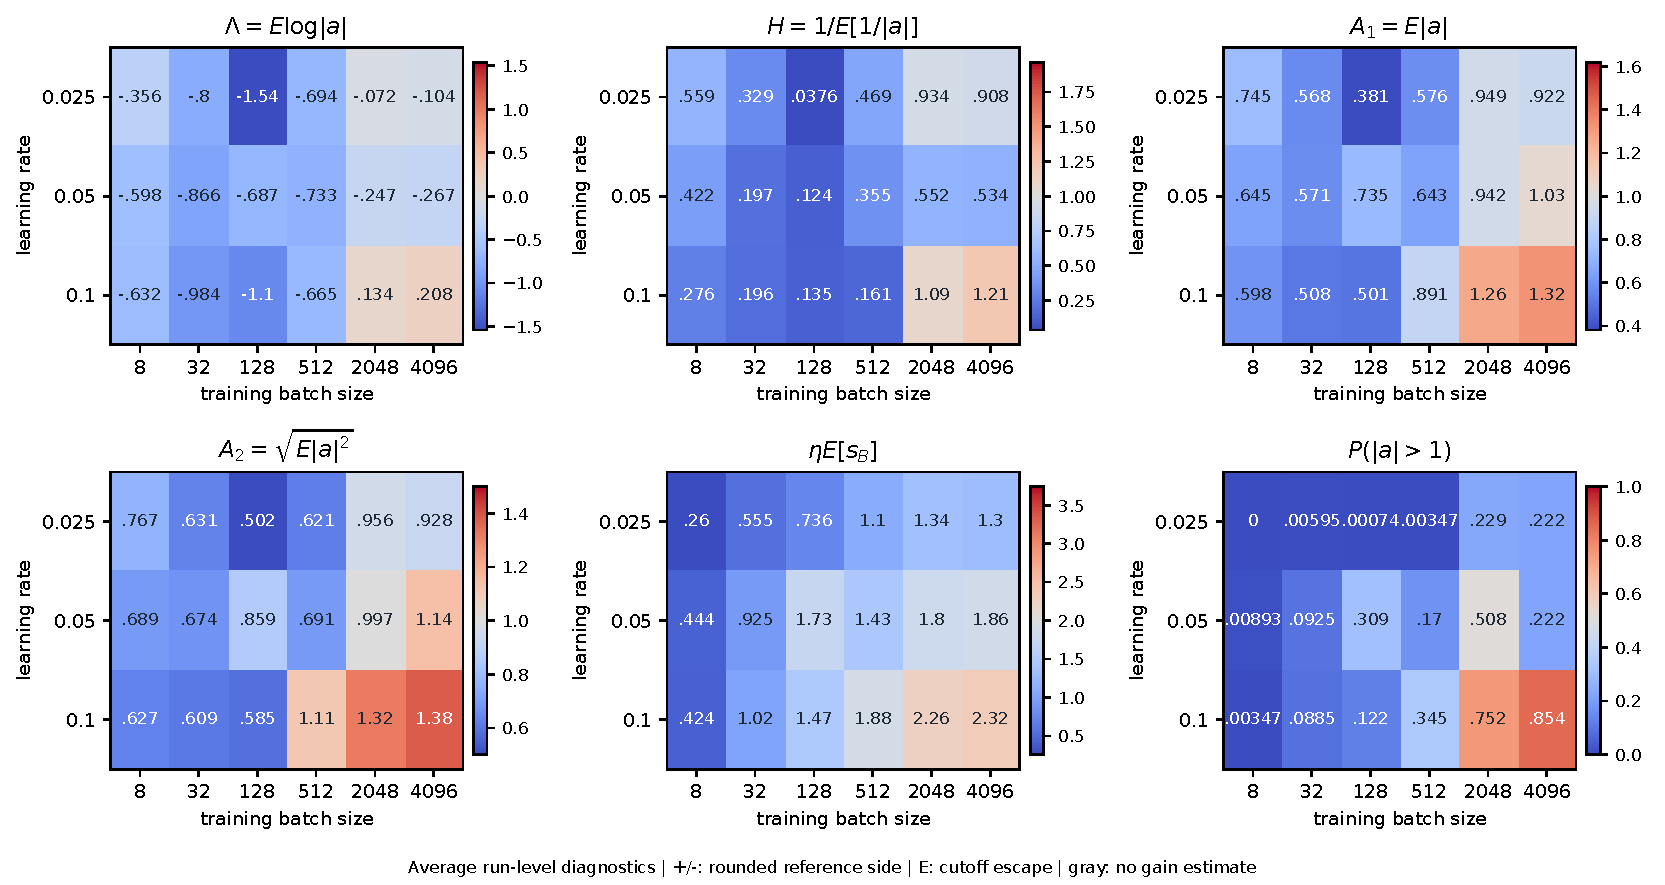
\includegraphics[width=\linewidth,height=0.78\textheight,keepaspectratio]{img/current_results/resnet32_grid_eta_batch.pdf}
\caption{\textbf{ResNet-32 without BatchNorm | stability grid over batch size and step size.} Axes are actual training learning rate and batch size. The six panels show Lambda, H, A1, A2, eta E[s\_B], and the fraction of expanding gains. Each cell averages run-level statistics from the final three available checkpoints; time windows can differ across settings and runs. Color centers are 0, 1, 1, 1, 2, and 0.5. Curvature and expansion-fraction centers are references, not full-network stability tests. A trailing +/- preserves the side of a reference after rounding. Gray means no gain estimate; E marks a recorded escape, including pre-escape estimates. Finite H does not establish population inverse-moment finiteness.}
\label{fig:current-resnet32-grid-eta-batch}
\end{figure}\clearpage

\begin{figure}[p]\centering
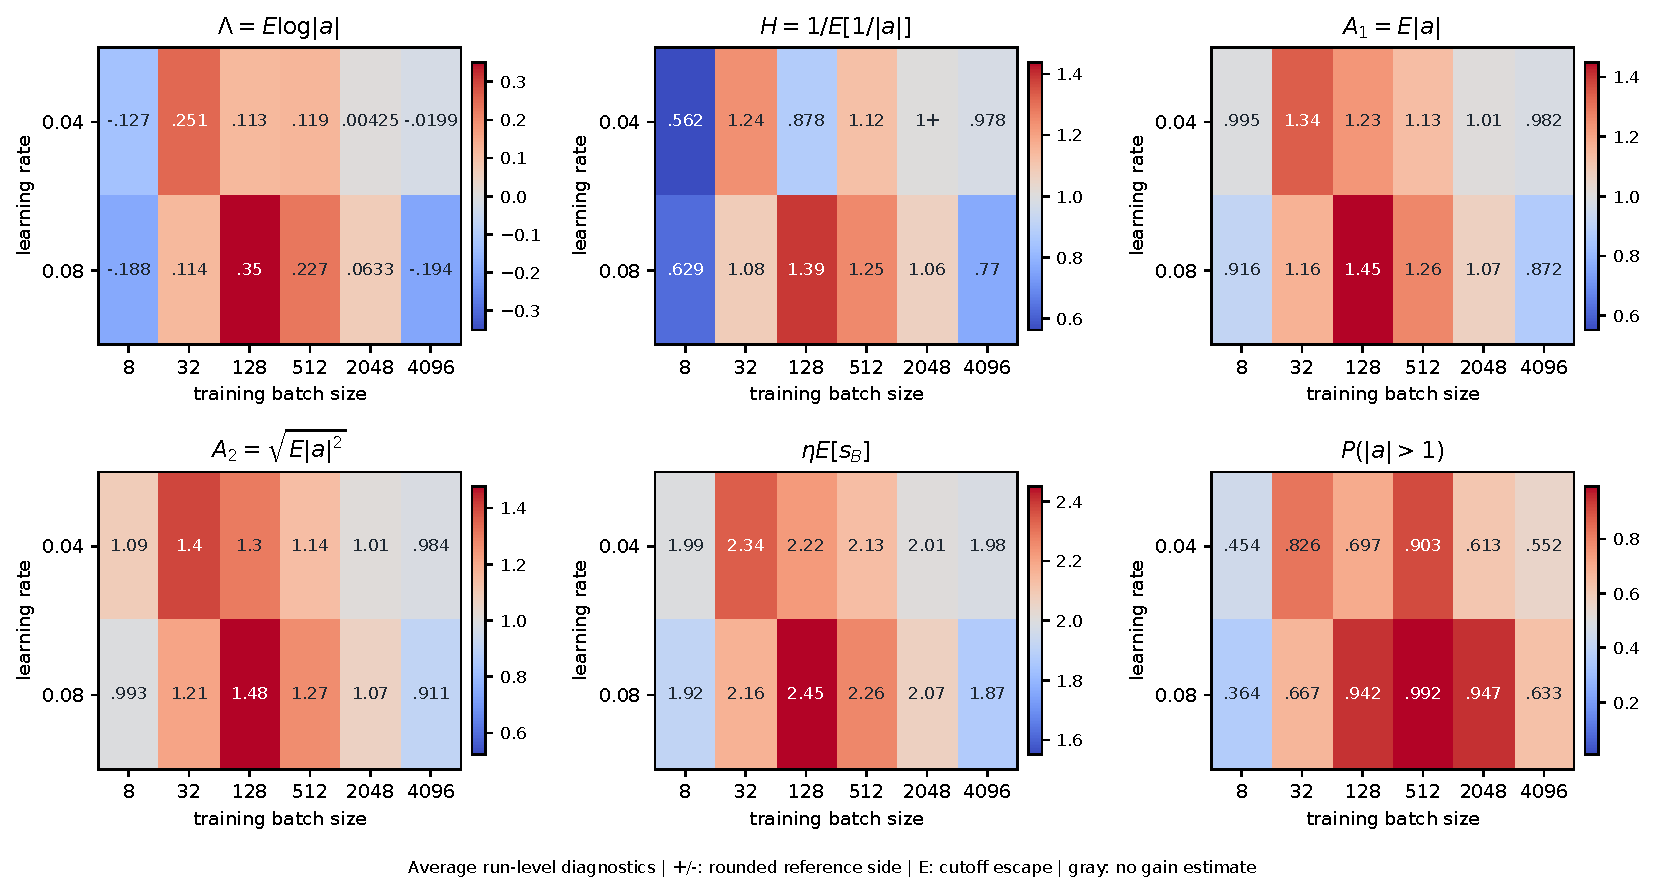
\includegraphics[width=\linewidth,height=0.78\textheight,keepaspectratio]{img/current_results/cnn_grid_eta_batch.pdf}
\caption{\textbf{CNN, 3 convolutional layers (ReLU) | stability grid over batch size and step size.} Axes are actual training learning rate and batch size. The six panels show Lambda, H, A1, A2, eta E[s\_B], and the fraction of expanding gains. Each cell averages run-level statistics from the final three available checkpoints; time windows can differ across settings and runs. Color centers are 0, 1, 1, 1, 2, and 0.5. Curvature and expansion-fraction centers are references, not full-network stability tests. A trailing +/- preserves the side of a reference after rounding. Gray means no gain estimate; E marks a recorded escape, including pre-escape estimates. Finite H does not establish population inverse-moment finiteness.}
\label{fig:current-cnn-grid-eta-batch}
\end{figure}\clearpage

\begin{figure}[p]\centering
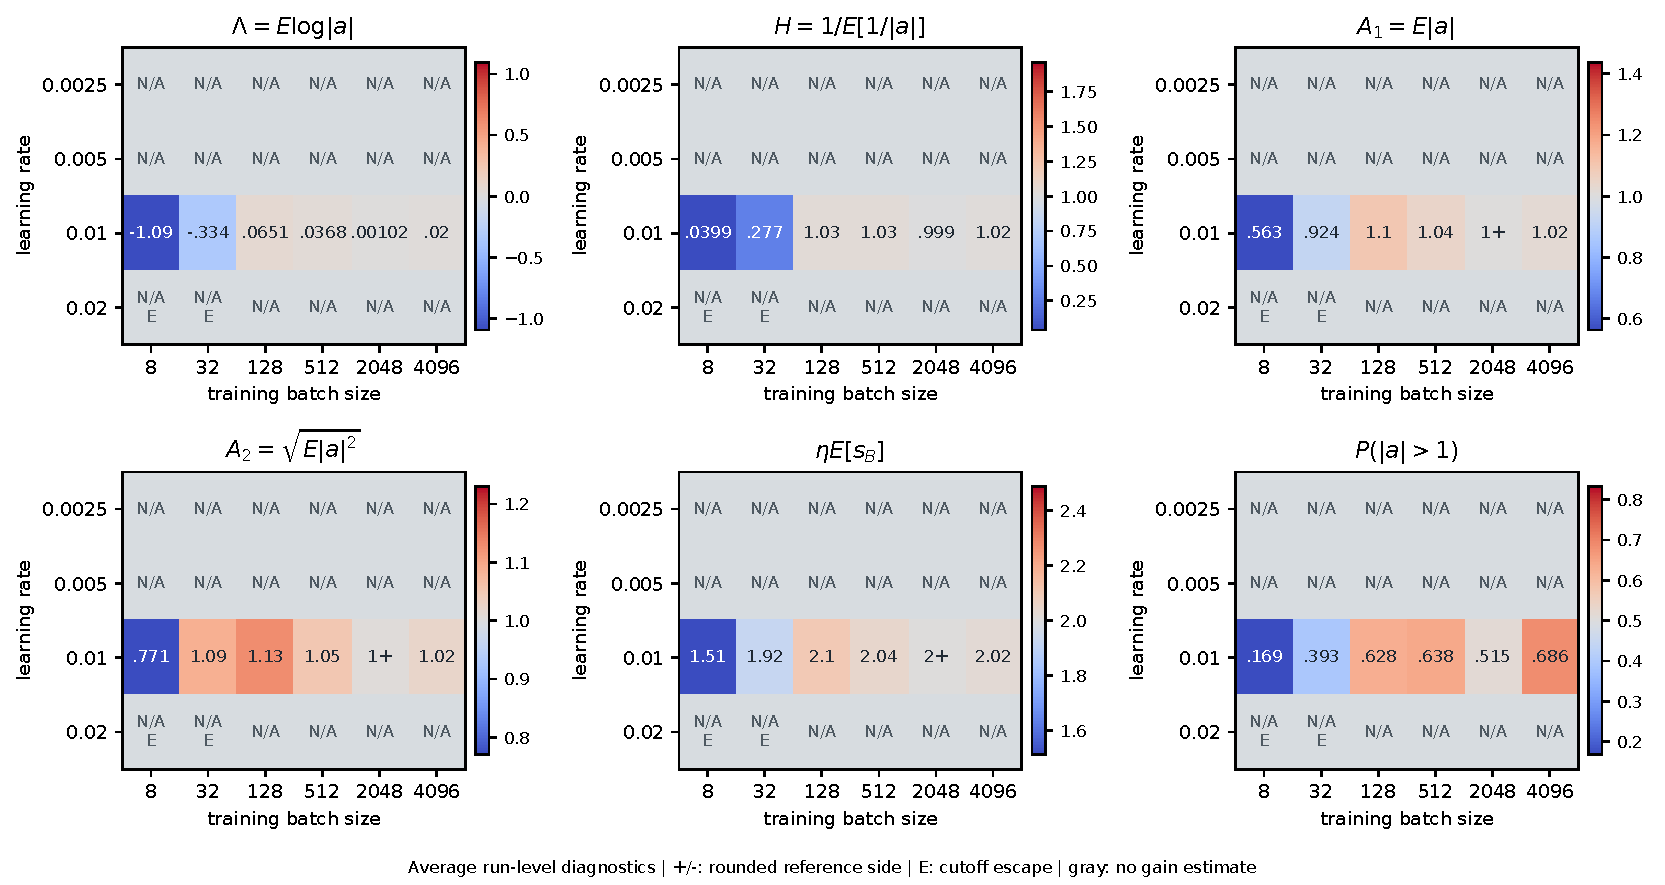
\includegraphics[width=\linewidth,height=0.78\textheight,keepaspectratio]{img/current_results/mlp_d1_grid_eta_batch.pdf}
\caption{\textbf{MLP, 1 x 256 (ReLU) | stability grid over batch size and step size.} Axes are actual training learning rate and batch size. The six panels show Lambda, H, A1, A2, eta E[s\_B], and the fraction of expanding gains. Each cell averages run-level statistics from the final three available checkpoints; time windows can differ across settings and runs. Color centers are 0, 1, 1, 1, 2, and 0.5. Curvature and expansion-fraction centers are references, not full-network stability tests. A trailing +/- preserves the side of a reference after rounding. Gray means no gain estimate; E marks a recorded escape, including pre-escape estimates. Finite H does not establish population inverse-moment finiteness.}
\label{fig:current-mlp-d1-grid-eta-batch}
\end{figure}\clearpage

\begin{figure}[p]\centering
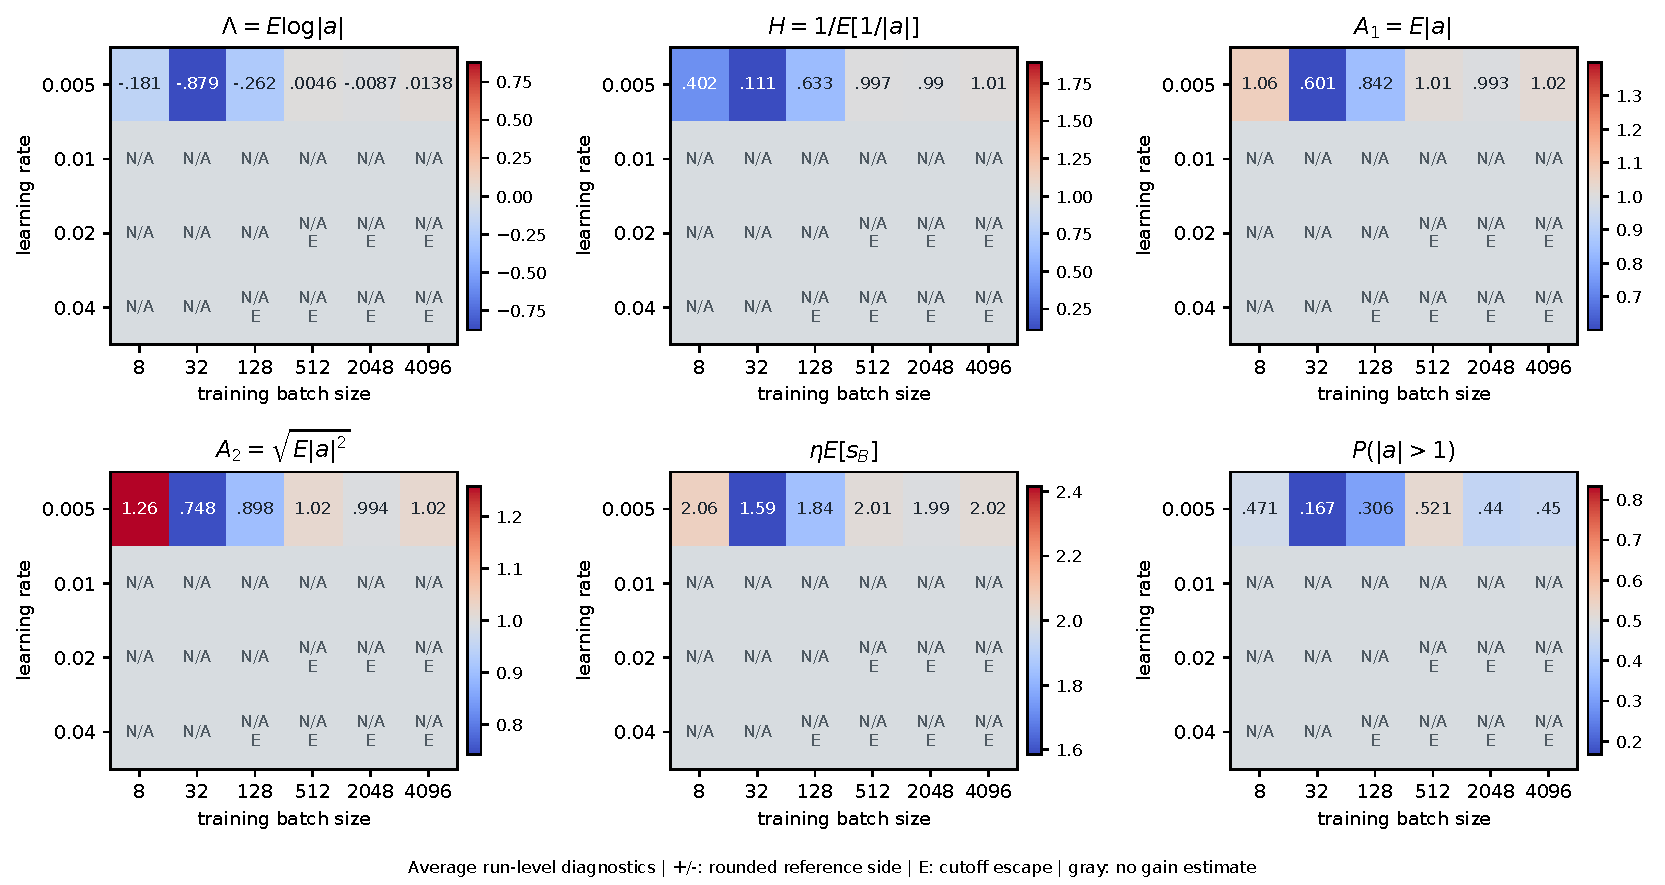
\includegraphics[width=\linewidth,height=0.78\textheight,keepaspectratio]{img/current_results/mlp_d2_grid_eta_batch.pdf}
\caption{\textbf{MLP, 2 x 512 (ReLU) | stability grid over batch size and step size.} Axes are actual training learning rate and batch size. The six panels show Lambda, H, A1, A2, eta E[s\_B], and the fraction of expanding gains. Each cell averages run-level statistics from the final three available checkpoints; time windows can differ across settings and runs. Color centers are 0, 1, 1, 1, 2, and 0.5. Curvature and expansion-fraction centers are references, not full-network stability tests. A trailing +/- preserves the side of a reference after rounding. Gray means no gain estimate; E marks a recorded escape, including pre-escape estimates. Finite H does not establish population inverse-moment finiteness.}
\label{fig:current-mlp-d2-grid-eta-batch}
\end{figure}\clearpage

\begin{figure}[p]\centering
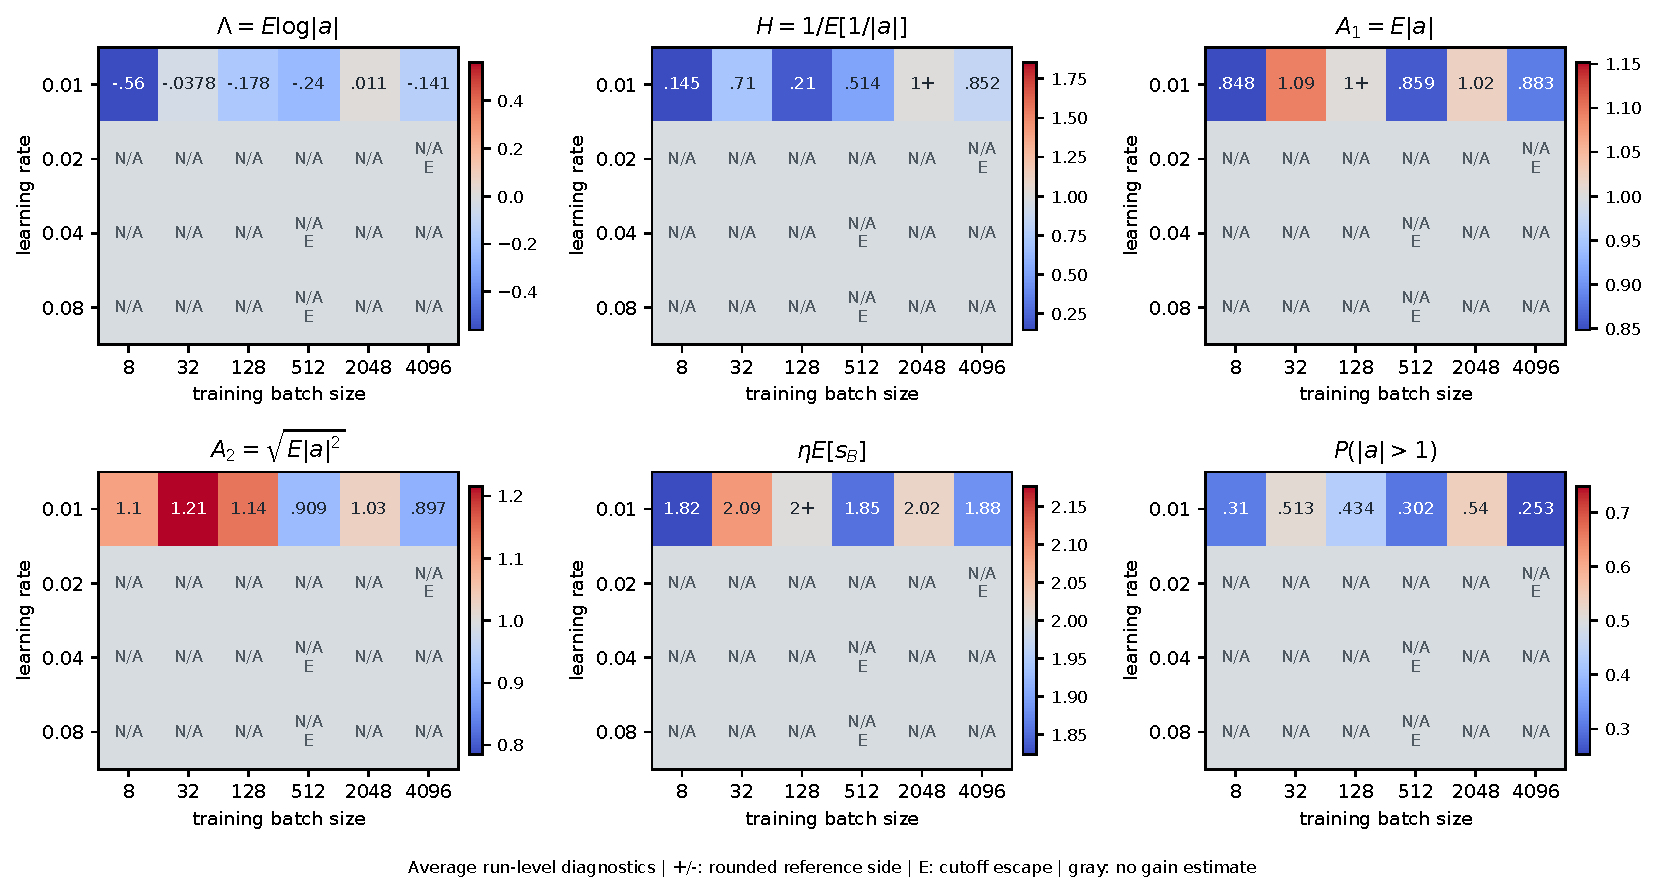
\includegraphics[width=\linewidth,height=0.78\textheight,keepaspectratio]{img/current_results/mlp_d3_grid_eta_batch.pdf}
\caption{\textbf{MLP, 3 x 256 (ReLU) | stability grid over batch size and step size.} Axes are actual training learning rate and batch size. The six panels show Lambda, H, A1, A2, eta E[s\_B], and the fraction of expanding gains. Each cell averages run-level statistics from the final three available checkpoints; time windows can differ across settings and runs. Color centers are 0, 1, 1, 1, 2, and 0.5. Curvature and expansion-fraction centers are references, not full-network stability tests. A trailing +/- preserves the side of a reference after rounding. Gray means no gain estimate; E marks a recorded escape, including pre-escape estimates. Finite H does not establish population inverse-moment finiteness.}
\label{fig:current-mlp-d3-grid-eta-batch}
\end{figure}\clearpage

\begin{figure}[p]\centering
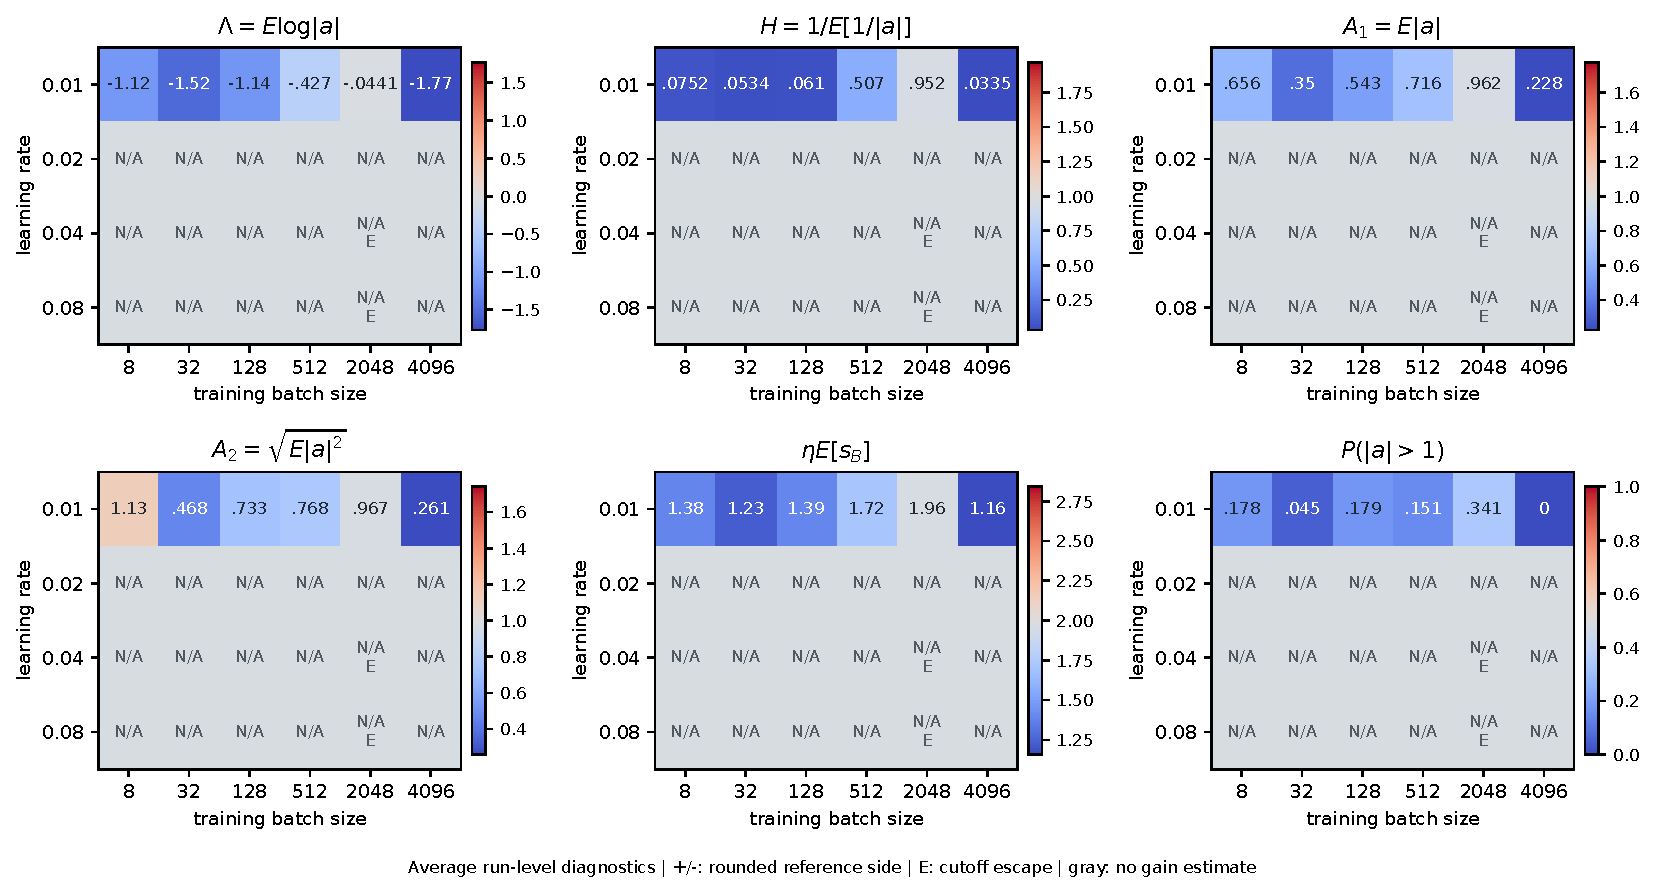
\includegraphics[width=\linewidth,height=0.78\textheight,keepaspectratio]{img/current_results/mlp_d4_grid_eta_batch.pdf}
\caption{\textbf{MLP, 4 x 512 (ReLU) | stability grid over batch size and step size.} Axes are actual training learning rate and batch size. The six panels show Lambda, H, A1, A2, eta E[s\_B], and the fraction of expanding gains. Each cell averages run-level statistics from the final three available checkpoints; time windows can differ across settings and runs. Color centers are 0, 1, 1, 1, 2, and 0.5. Curvature and expansion-fraction centers are references, not full-network stability tests. A trailing +/- preserves the side of a reference after rounding. Gray means no gain estimate; E marks a recorded escape, including pre-escape estimates. Finite H does not establish population inverse-moment finiteness.}
\label{fig:current-mlp-d4-grid-eta-batch}
\end{figure}\clearpage

\begin{figure}[p]\centering
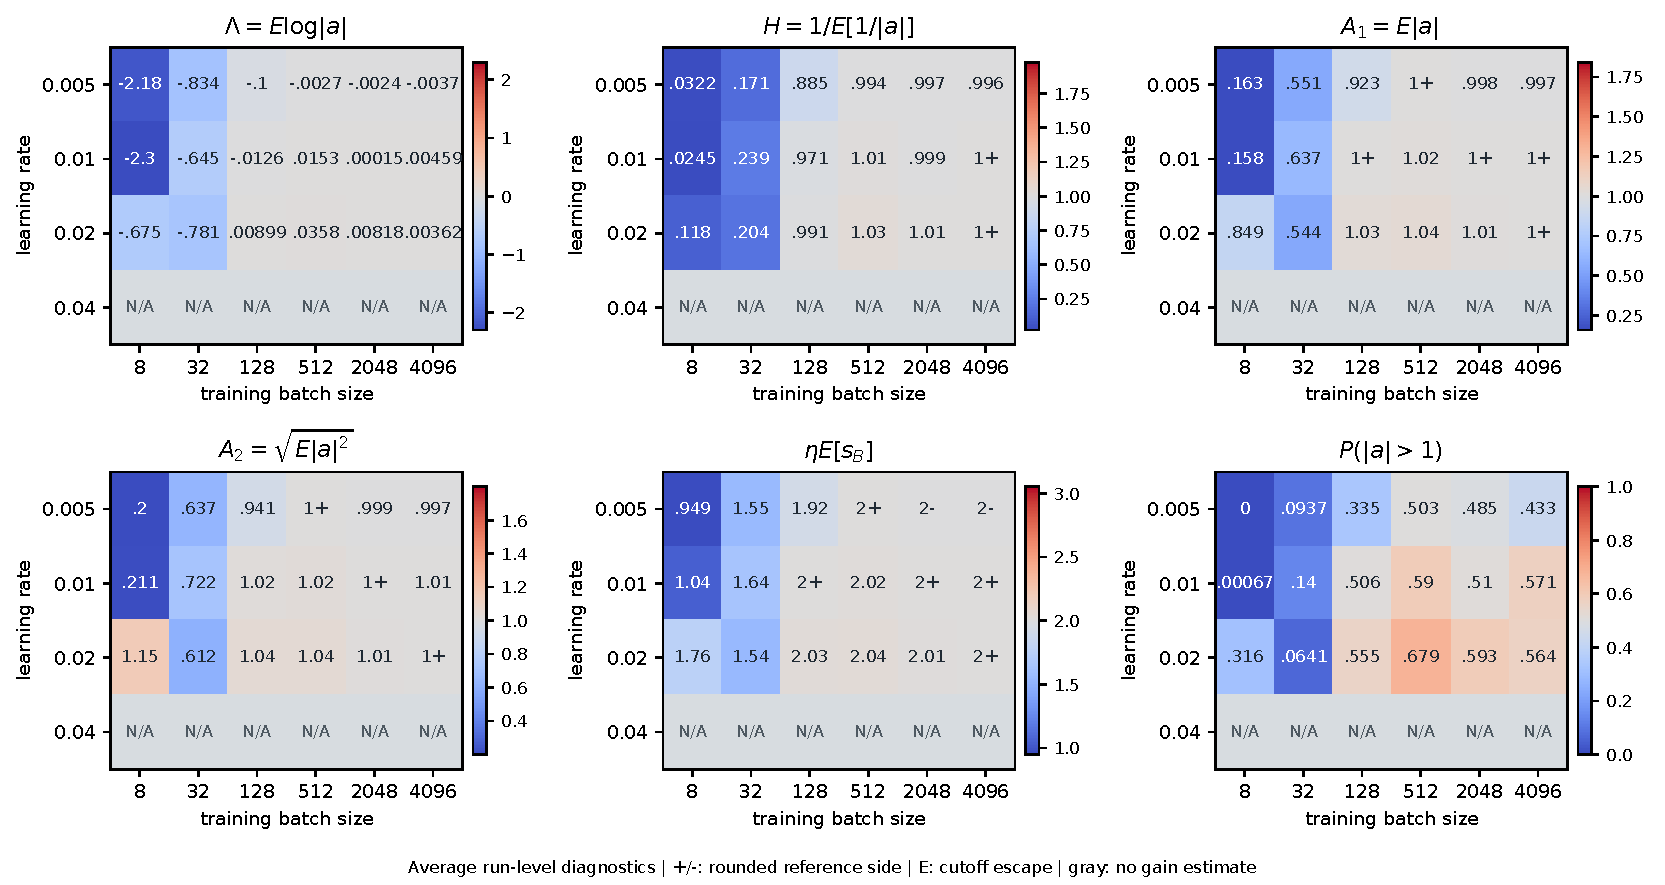
\includegraphics[width=\linewidth,height=0.78\textheight,keepaspectratio]{img/current_results/mlp_tanh_grid_eta_batch.pdf}
\caption{\textbf{MLP, 2 x 512 (tanh) | stability grid over batch size and step size.} Axes are actual training learning rate and batch size. The six panels show Lambda, H, A1, A2, eta E[s\_B], and the fraction of expanding gains. Each cell averages run-level statistics from the final three available checkpoints; time windows can differ across settings and runs. Color centers are 0, 1, 1, 1, 2, and 0.5. Curvature and expansion-fraction centers are references, not full-network stability tests. A trailing +/- preserves the side of a reference after rounding. Gray means no gain estimate; E marks a recorded escape, including pre-escape estimates. Finite H does not establish population inverse-moment finiteness.}
\label{fig:current-mlp-tanh-grid-eta-batch}
\end{figure}\clearpage

\begin{figure}[p]\centering
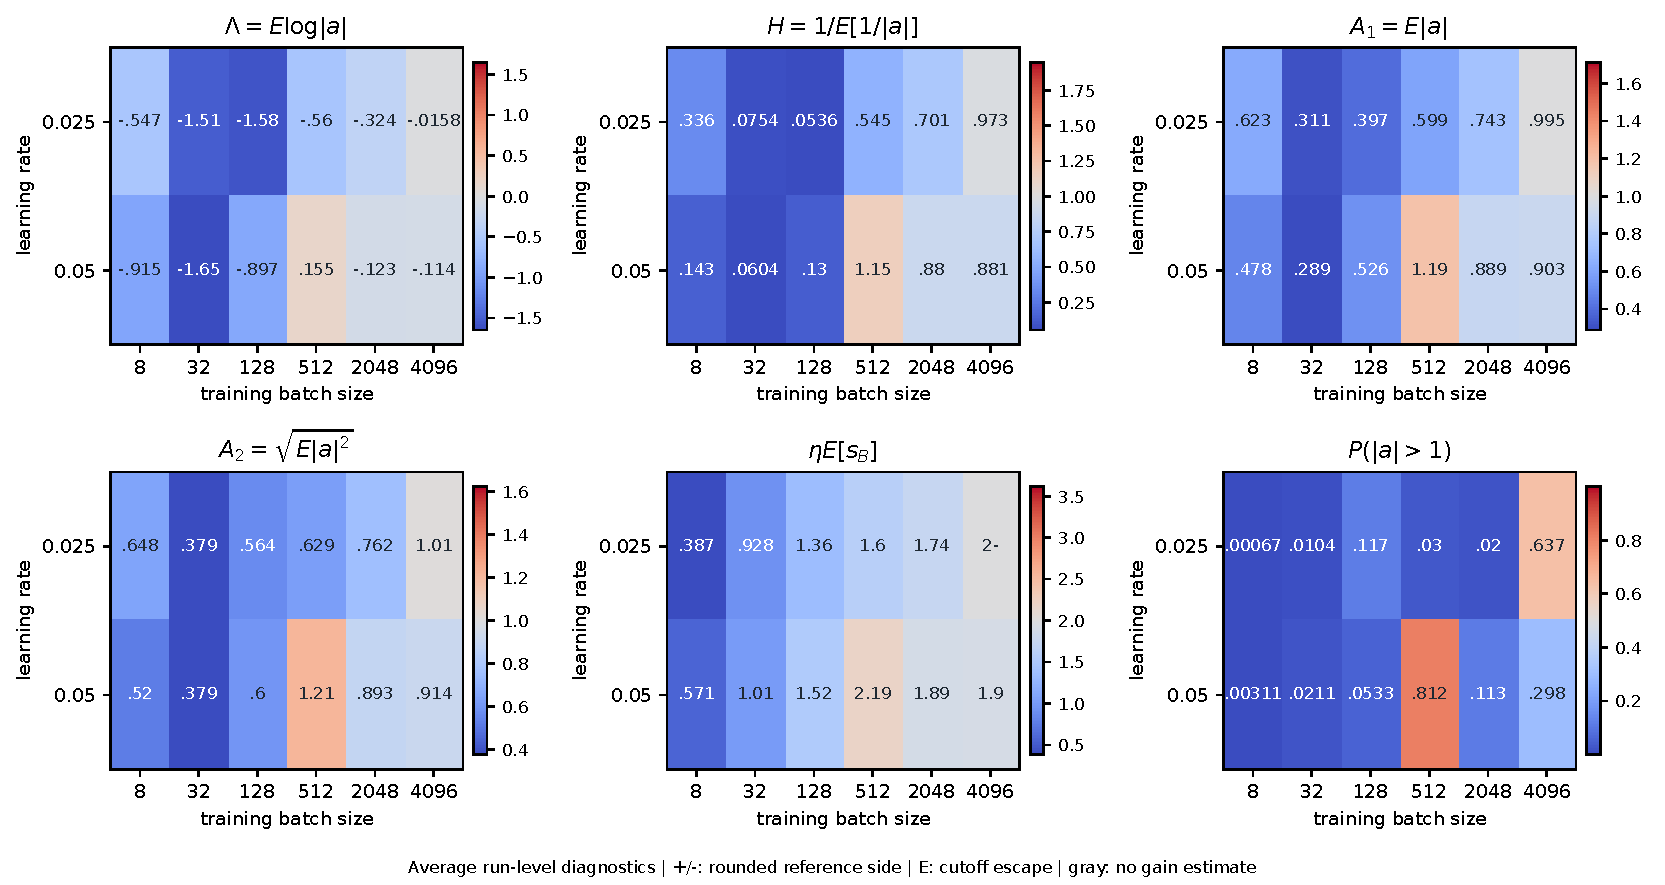
\includegraphics[width=\linewidth,height=0.78\textheight,keepaspectratio]{img/current_results/resnet20_grid_eta_batch.pdf}
\caption{\textbf{ResNet-20 without BatchNorm | stability grid over batch size and step size.} Axes are actual training learning rate and batch size. The six panels show Lambda, H, A1, A2, eta E[s\_B], and the fraction of expanding gains. Each cell averages run-level statistics from the final three available checkpoints; time windows can differ across settings and runs. Color centers are 0, 1, 1, 1, 2, and 0.5. Curvature and expansion-fraction centers are references, not full-network stability tests. A trailing +/- preserves the side of a reference after rounding. Gray means no gain estimate; E marks a recorded escape, including pre-escape estimates. Finite H does not establish population inverse-moment finiteness.}
\label{fig:current-resnet20-grid-eta-batch}
\end{figure}\clearpage

\begin{figure}[p]\centering
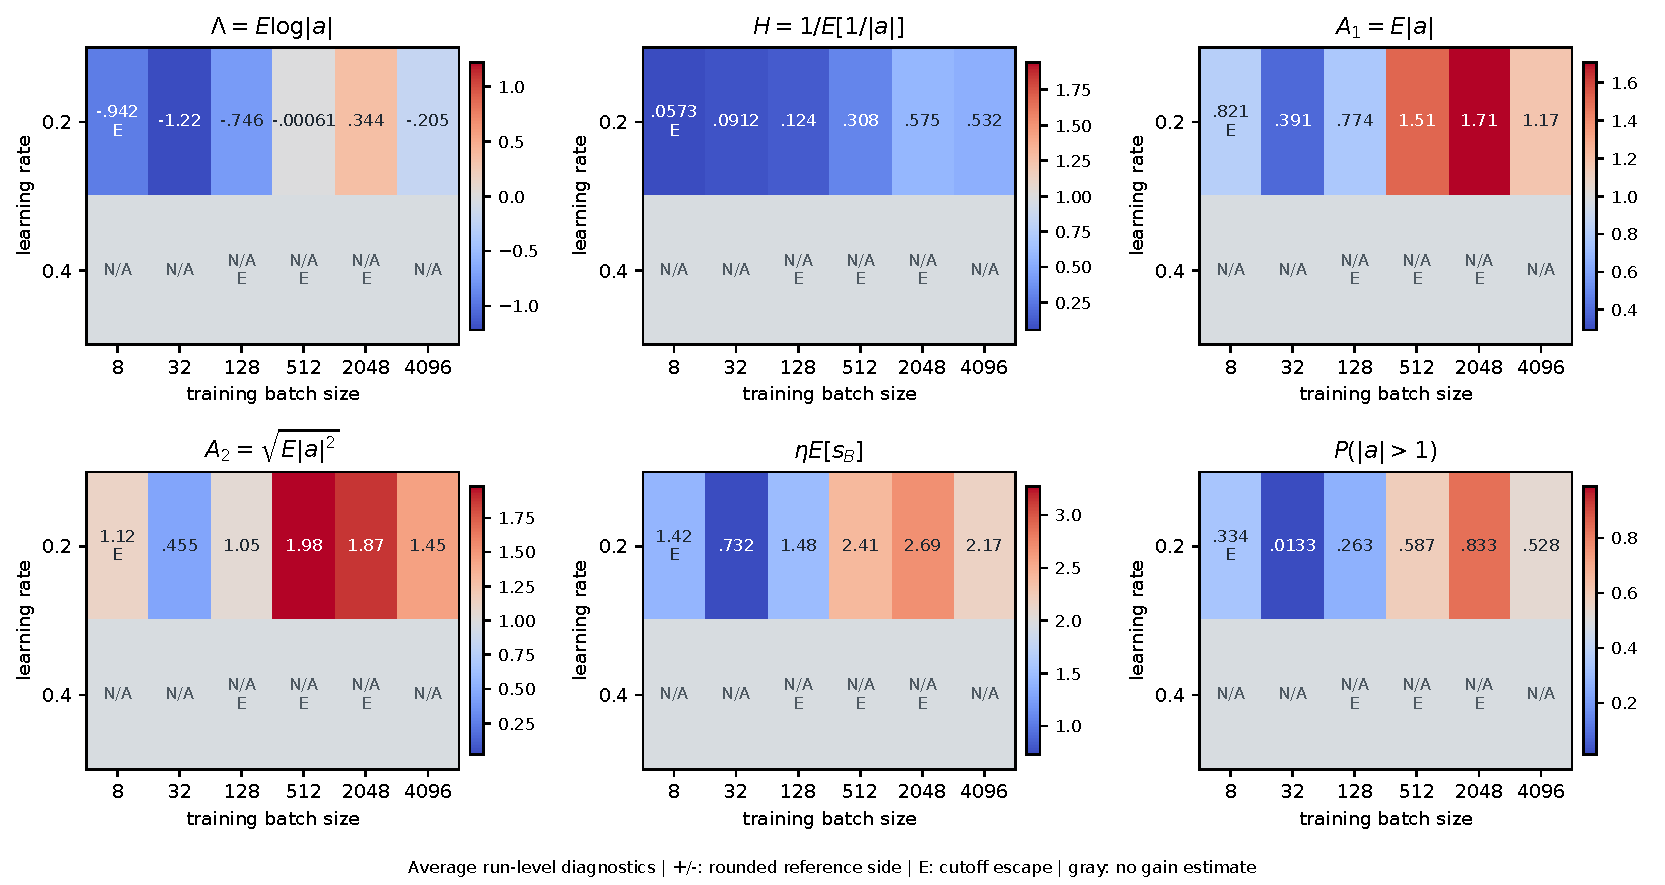
\includegraphics[width=\linewidth,height=0.78\textheight,keepaspectratio]{img/current_results/vit_grid_eta_batch.pdf}
\caption{\textbf{ViT, 2 blocks x width 64 | stability grid over batch size and step size.} Axes are actual training learning rate and batch size. The six panels show Lambda, H, A1, A2, eta E[s\_B], and the fraction of expanding gains. Each cell averages run-level statistics from the final three available checkpoints; time windows can differ across settings and runs. Color centers are 0, 1, 1, 1, 2, and 0.5. Curvature and expansion-fraction centers are references, not full-network stability tests. A trailing +/- preserves the side of a reference after rounding. Gray means no gain estimate; E marks a recorded escape, including pre-escape estimates. Finite H does not establish population inverse-moment finiteness.}
\label{fig:current-vit-grid-eta-batch}
\end{figure}\clearpage

\begin{figure}[p]\centering
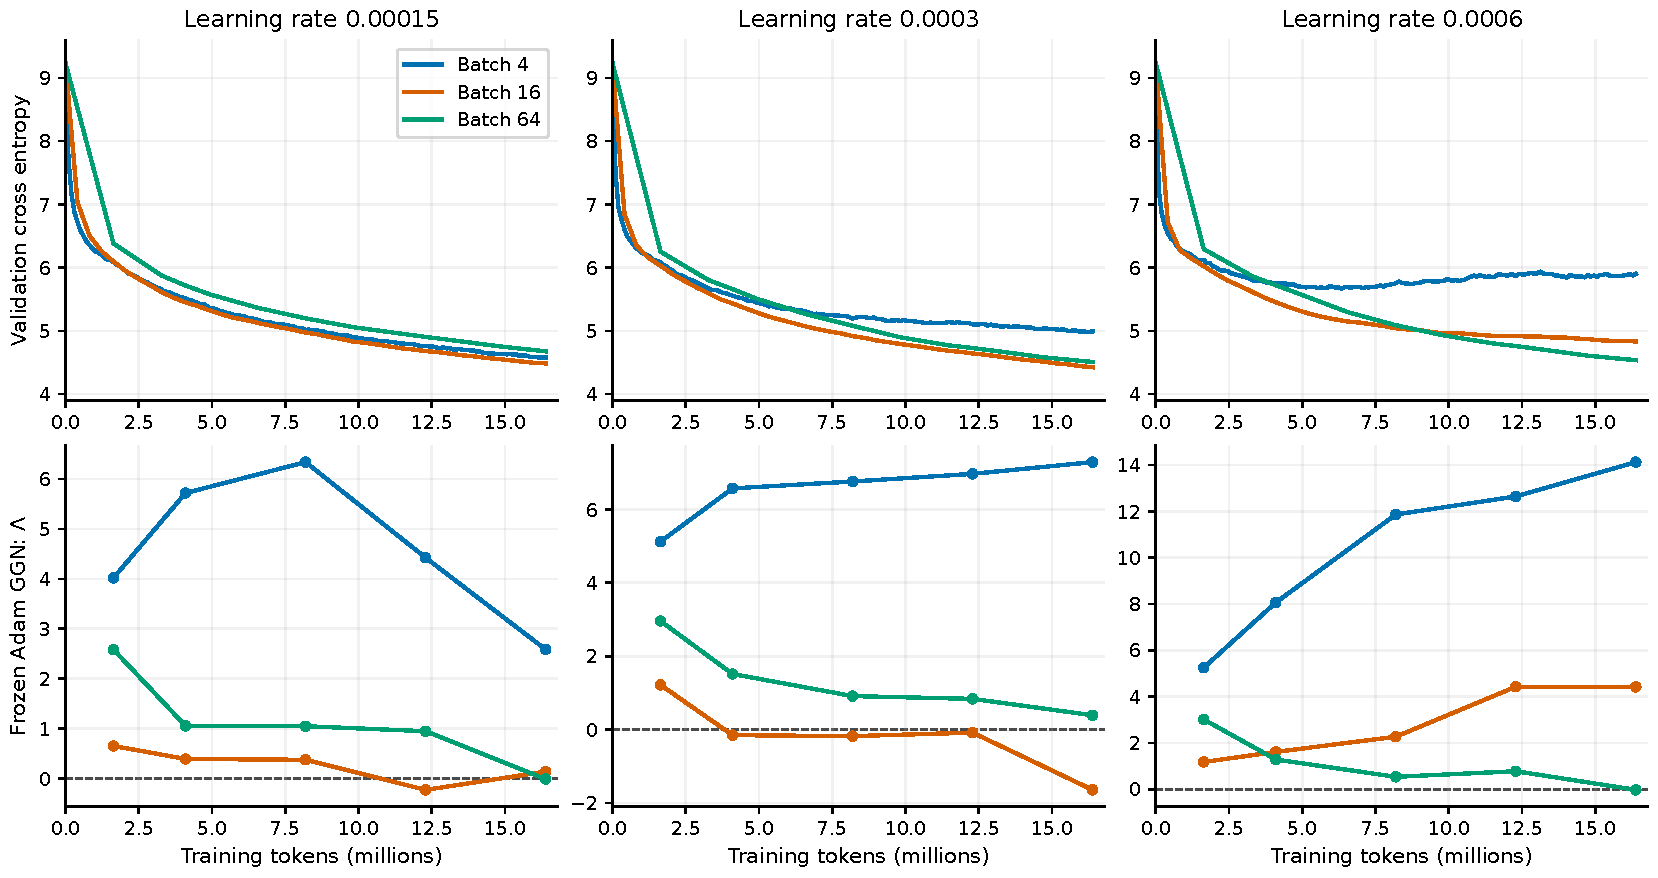
\includegraphics[width=\linewidth,height=0.78\textheight,keepaspectratio]{img/current_results/gpt01_token_dynamics.pdf}
\caption{\textbf{GPT / FineWeb-Edu: loss improves while frozen scalar growth can expand.} Columns compare learning rates and colors compare effective batches in sequences. Top: validation-window Monte Carlo loss along training. Bottom: matched-parent-batch frozen-Adam GGN scalar Lambda = mean(log|1-eta s|), measured on 8 fresh probe batches at each checkpoint. Lines show average run-level estimates. All parent optimizers use Adam; the frozen diagnostic excludes momentum and preconditioner evolution. Positive scalar Lambda is not a full Adam Lyapunov exponent. Warmup occupies the first 10\% of tokens.}
\label{fig:current-gpt01-token-dynamics}
\end{figure}\clearpage

\begin{figure}[p]\centering
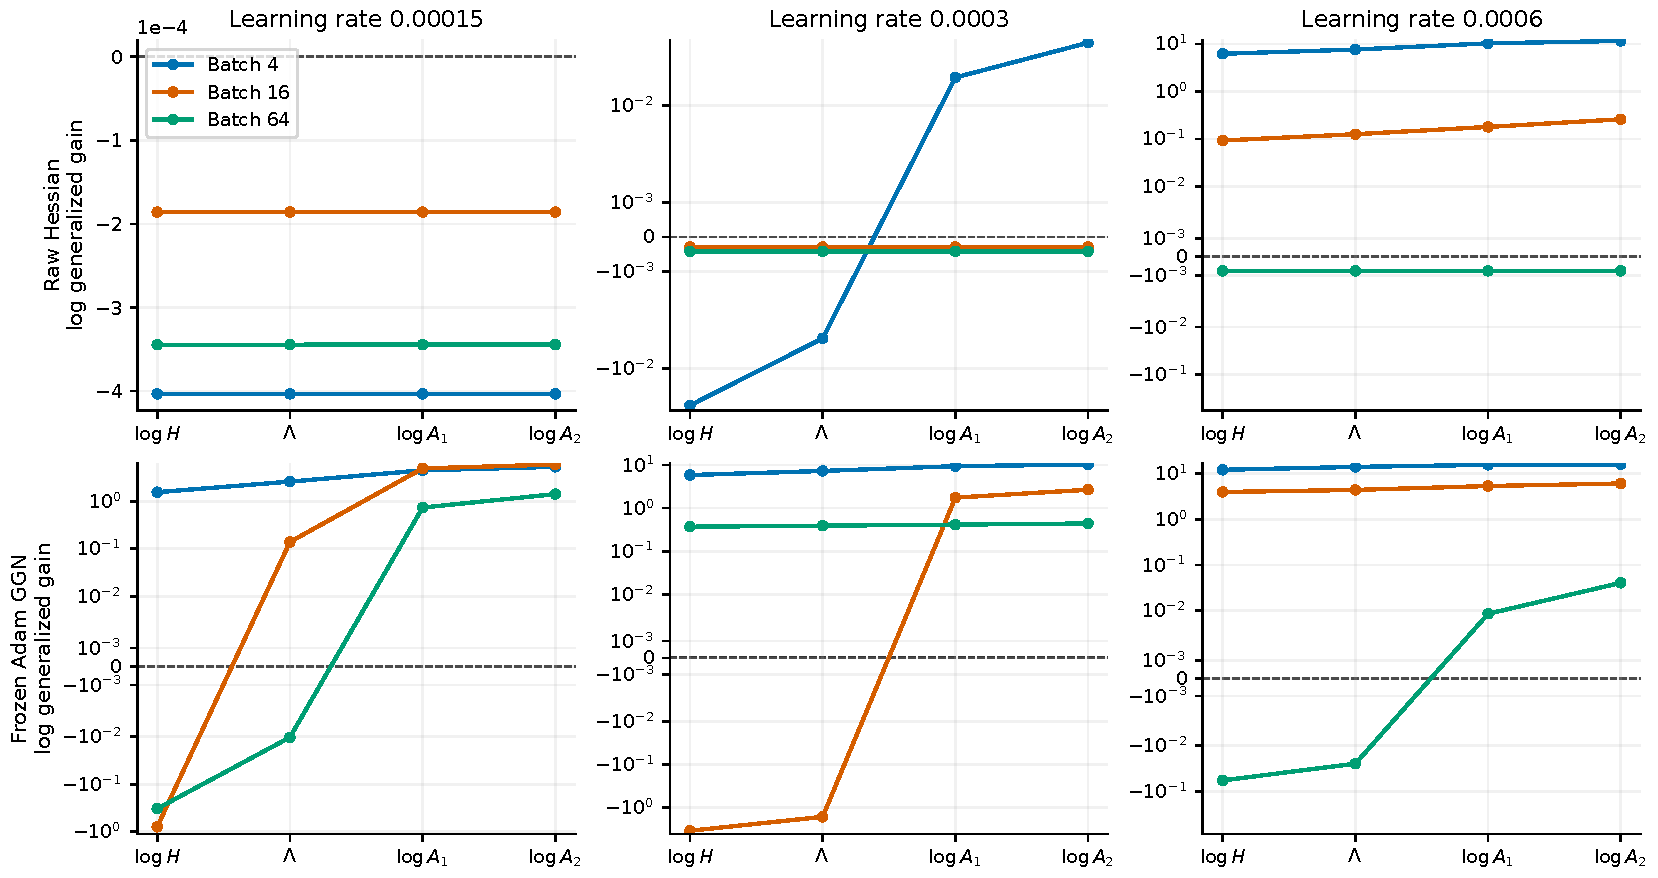
\includegraphics[width=\linewidth,height=0.78\textheight,keepaspectratio]{img/current_results/gpt02_moment_ladder.pdf}
\caption{\textbf{GPT / FineWeb-Edu: the apparent edge depends on moment and metric.} Final checkpoint only, with probe batch equal to parent batch. H=1/mean(|a|\textasciicircum{}-1), Lambda=mean(log|a|), A1=mean(|a|), A2=sqrt(mean(|a|\textasciicircum{}2)); each transformed quantity crosses its empirical boundary at zero. Vertical scales are symmetric-log except for the entirely near-zero top-left panel, which is linear. Every statistic is computed separately within a run; the displayed log statistics are then averaged. Raw Hessian uses 16 probes and frozen GGN 8. These finite-sample moment summaries do not establish population inverse-moment existence, an invariant distribution, or a full-optimizer boundary.}
\label{fig:current-gpt02-moment-ladder}
\end{figure}\clearpage

\begin{figure}[p]\centering
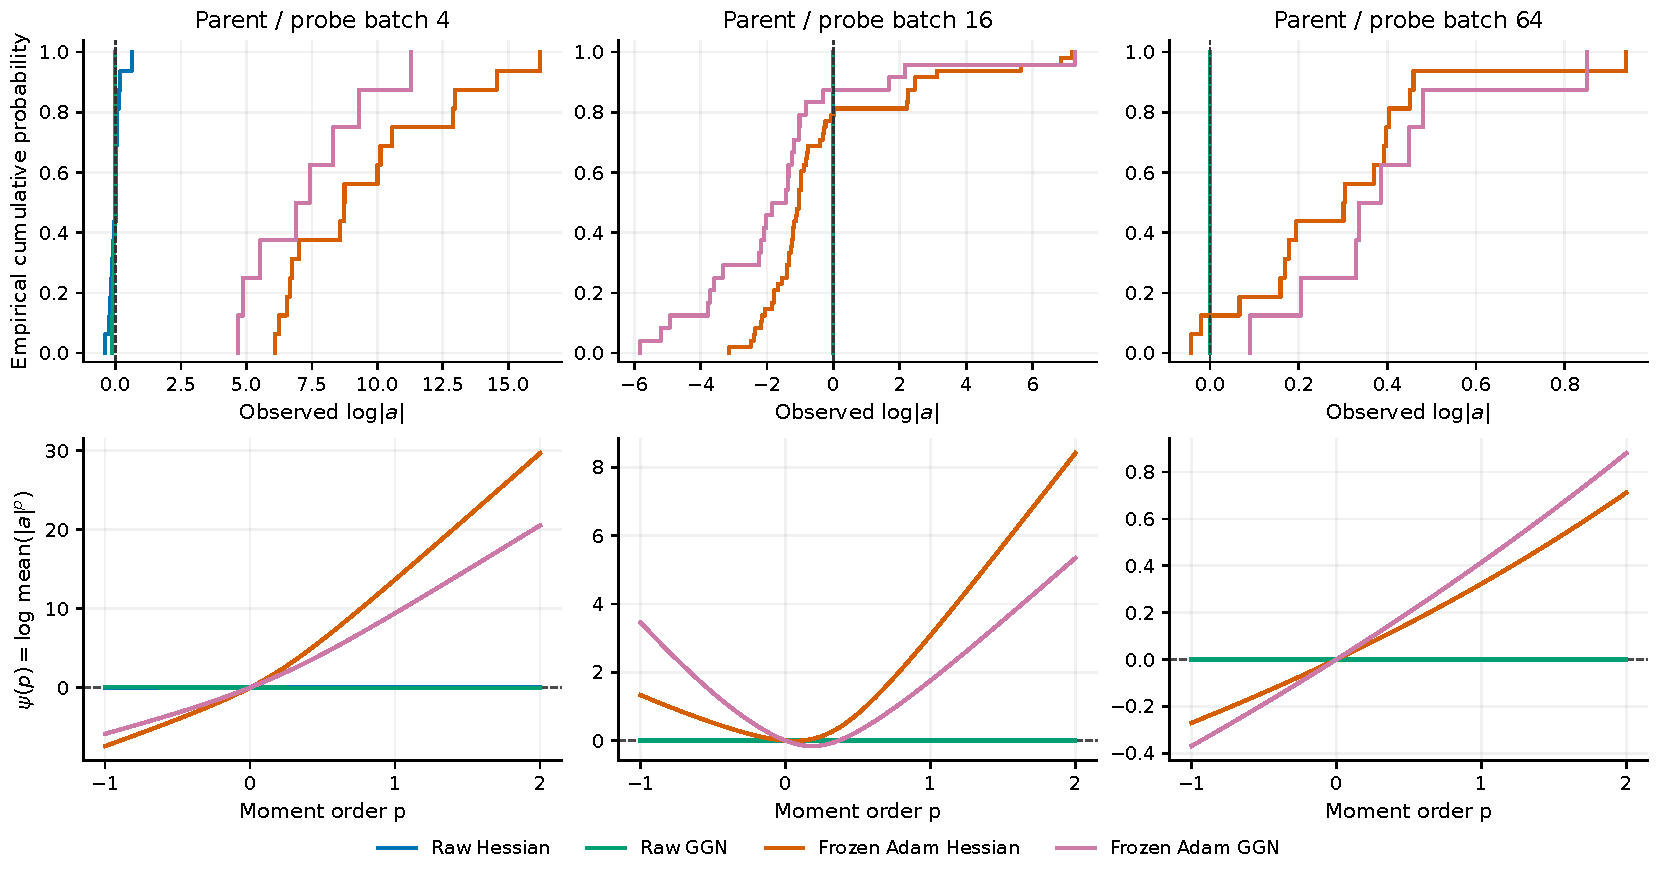
\includegraphics[width=\linewidth,height=0.78\textheight,keepaspectratio]{img/current_results/gpt03_gain_law.pdf}
\caption{\textbf{GPT / FineWeb-Edu: a few large gains change positive moments.} Eta 0.0003; final checkpoint and matched parent/probe batch. Top: empirical cumulative distribution of log absolute scalar gain. Bottom: empirical log moment function over p in [-1,2], with psi(0)=0 by identity. Raw and frozen Hessian use 16 probes per run, GGN uses 8. Lines are pointwise averages of run-level CDFs and moment curves, without merging raw samples across runs or checkpoints. Gain distributions are not distributions of model coordinates, so these panels do not establish bimodality.}
\label{fig:current-gpt03-gain-law}
\end{figure}\clearpage

\begin{figure}[p]\centering
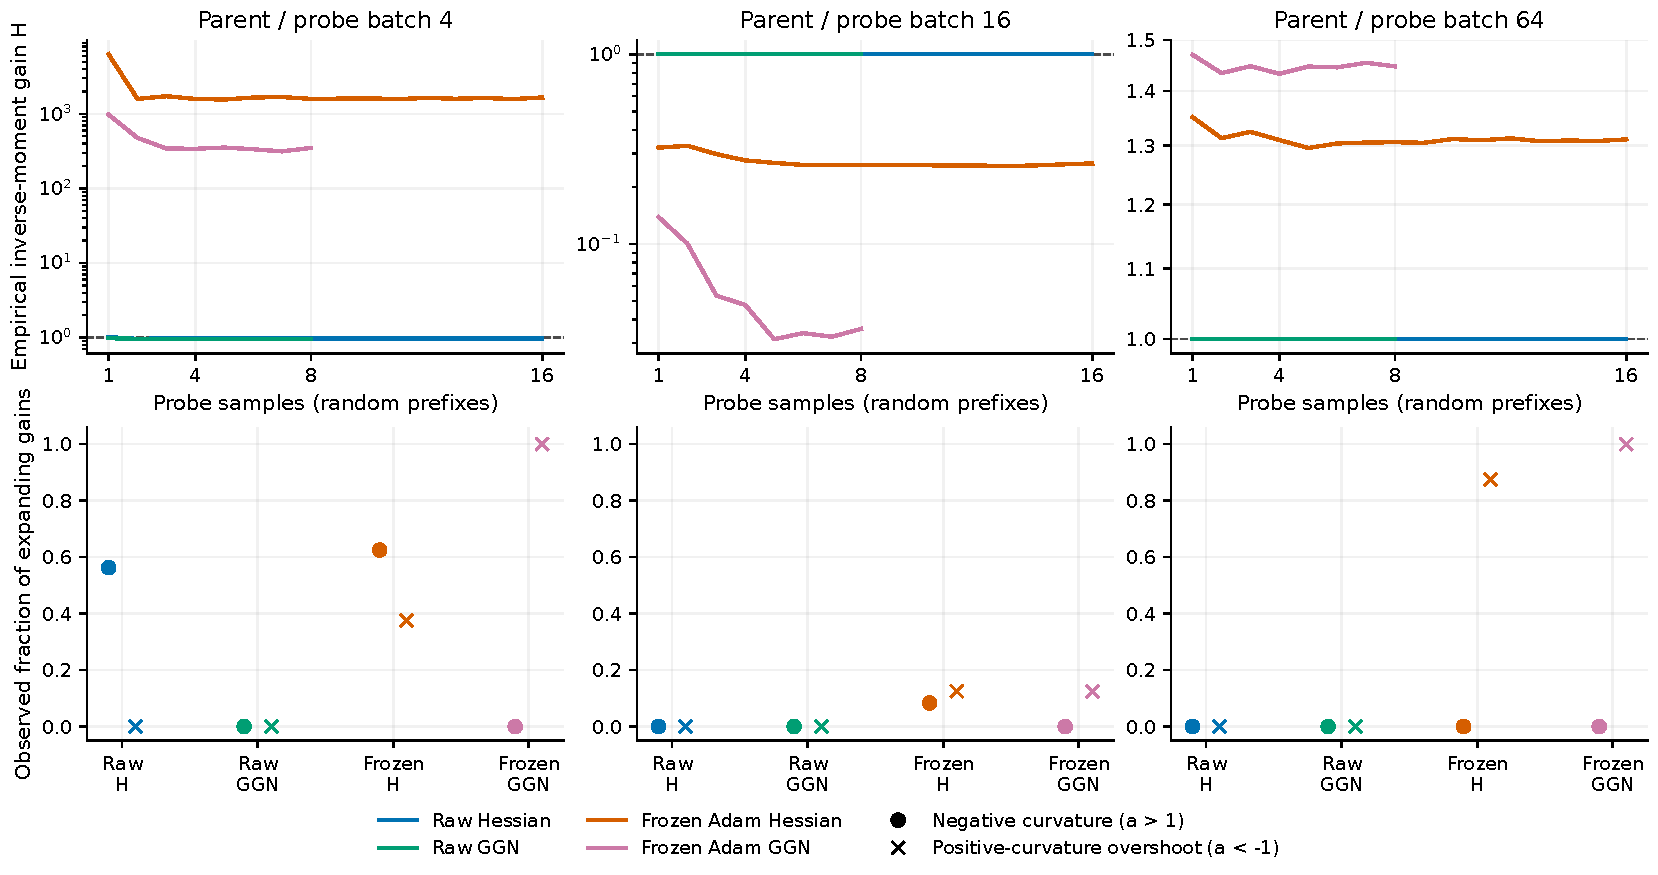
\includegraphics[width=\linewidth,height=0.78\textheight,keepaspectratio]{img/current_results/gpt04_inverse_and_mechanism.pdf}
\caption{\textbf{GPT / FineWeb-Edu: inverse moments and the cause of expansion need separate checks.} Eta 0.0003; final checkpoint and matched parent/probe batch. Top: median H over 256 randomized sample orders for each prefix size, computed separately per run; the line averages these medians. Prefix reshuffling is a sensitivity diagnostic, not new independent data or proof of inverse-moment convergence. Bottom: expansion caused by negative curvature (a>1) versus positive-curvature overshoot (a<-1), with average run-level fractions. GGN is positive semidefinite, so its expansion is from overshoot. Colors retain the four distinct scalar metric definitions.}
\label{fig:current-gpt04-inverse-and-mechanism}
\end{figure}\clearpage

\begin{figure}[p]\centering
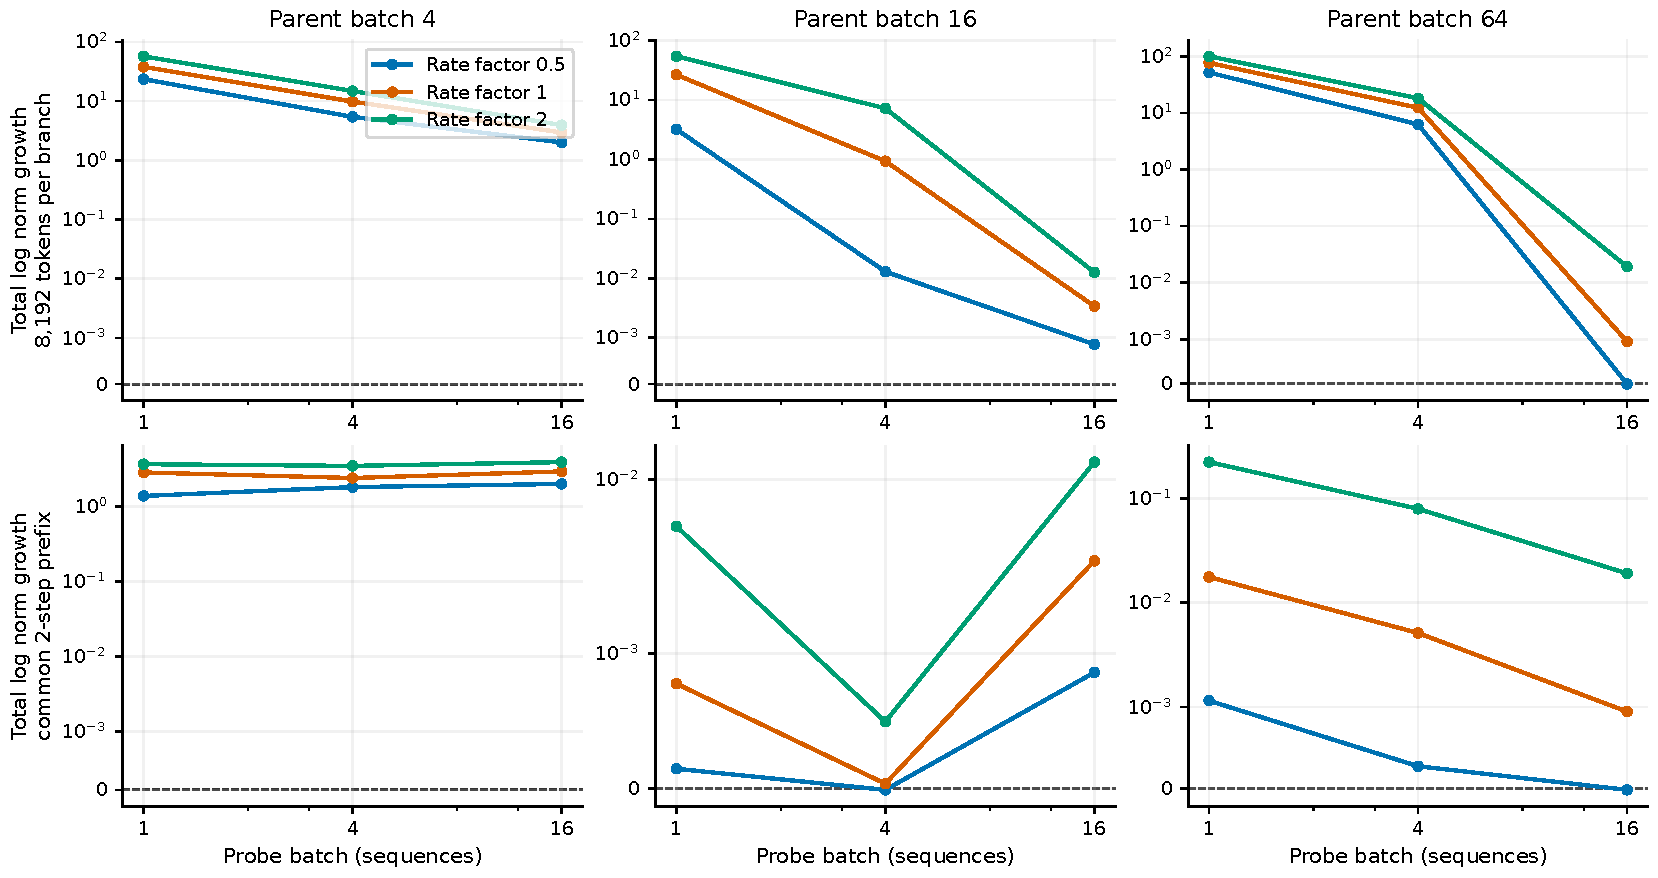
\includegraphics[width=\linewidth,height=0.78\textheight,keepaspectratio]{img/current_results/gpt05_matrix_control.pdf}
\caption{\textbf{GPT / FineWeb-Edu: token-matched matrix probes reveal growth missed by short prefixes.} Existing final-checkpoint frozen-Adam GGN matrix controls for eta0.0003 parents: propagate u by (I-eta D\textasciicircum{}(1/2) G\_B D\textasciicircum{}(1/2)) without resetting its direction and sum the log norms. Top gives each cell the same 8,192 tokens (32,8,2 steps at probe batches1,4,16); bottom uses only the common first2 steps. Curves average the available parent/probe-stream measurements. Rate factors are relative to parent eta0.0003. These finite-horizon, fixed-checkpoint matrix products exclude Adam momentum and evolution of D; they are not a full Adam Jacobian, asymptotic Lyapunov exponent, or nonlinear stability certificate.}
\label{fig:current-gpt05-matrix-control}
\end{figure}\clearpage

\begin{figure}[p]\centering
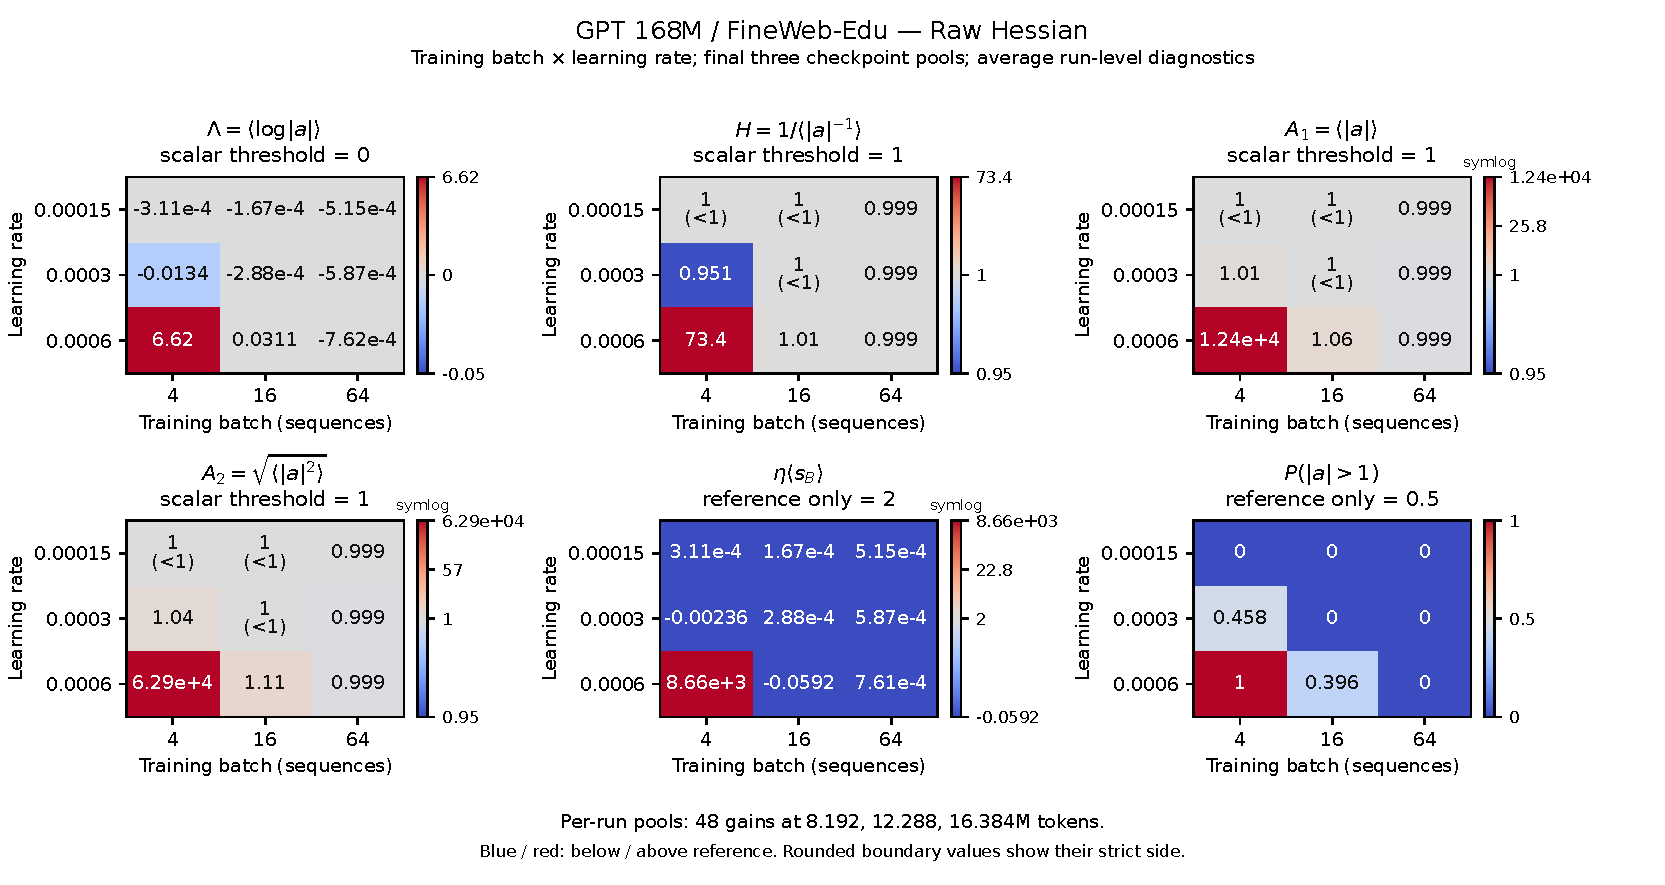
\includegraphics[width=\linewidth,height=0.78\textheight,keepaspectratio]{img/current_results/gpt_grid01_raw_hessian.pdf}
\caption{\textbf{GPT / FineWeb-Edu: batch--step-size grid, raw hessian.} Raw Hessian; all nine batch-rate cells retained. Values average run-level statistics from final-three-checkpoint pools at 8.192, 12.288 and 16.384 million tokens. Blue/red means below/above the panel reference. Pools contain 48 Hessian or 24 GGN gains per run. Annotations use three significant figures, with strict inequalities when rounded to a threshold. Symlog colorbars retain extreme values; ticks use original units. Eta E[s\_B]=2 and P(|a|>1)=0.5 are references, not stability certificates. Small inverse-moment samples do not establish population finiteness or stationarity. Parents use Adam: raw metrics are scalar SGD counterfactuals; frozen metrics exclude momentum and preconditioner evolution. Neither is a full-Adam Jacobian.}
\label{fig:current-gpt-grid01-raw-hessian}
\end{figure}\clearpage

\begin{figure}[p]\centering
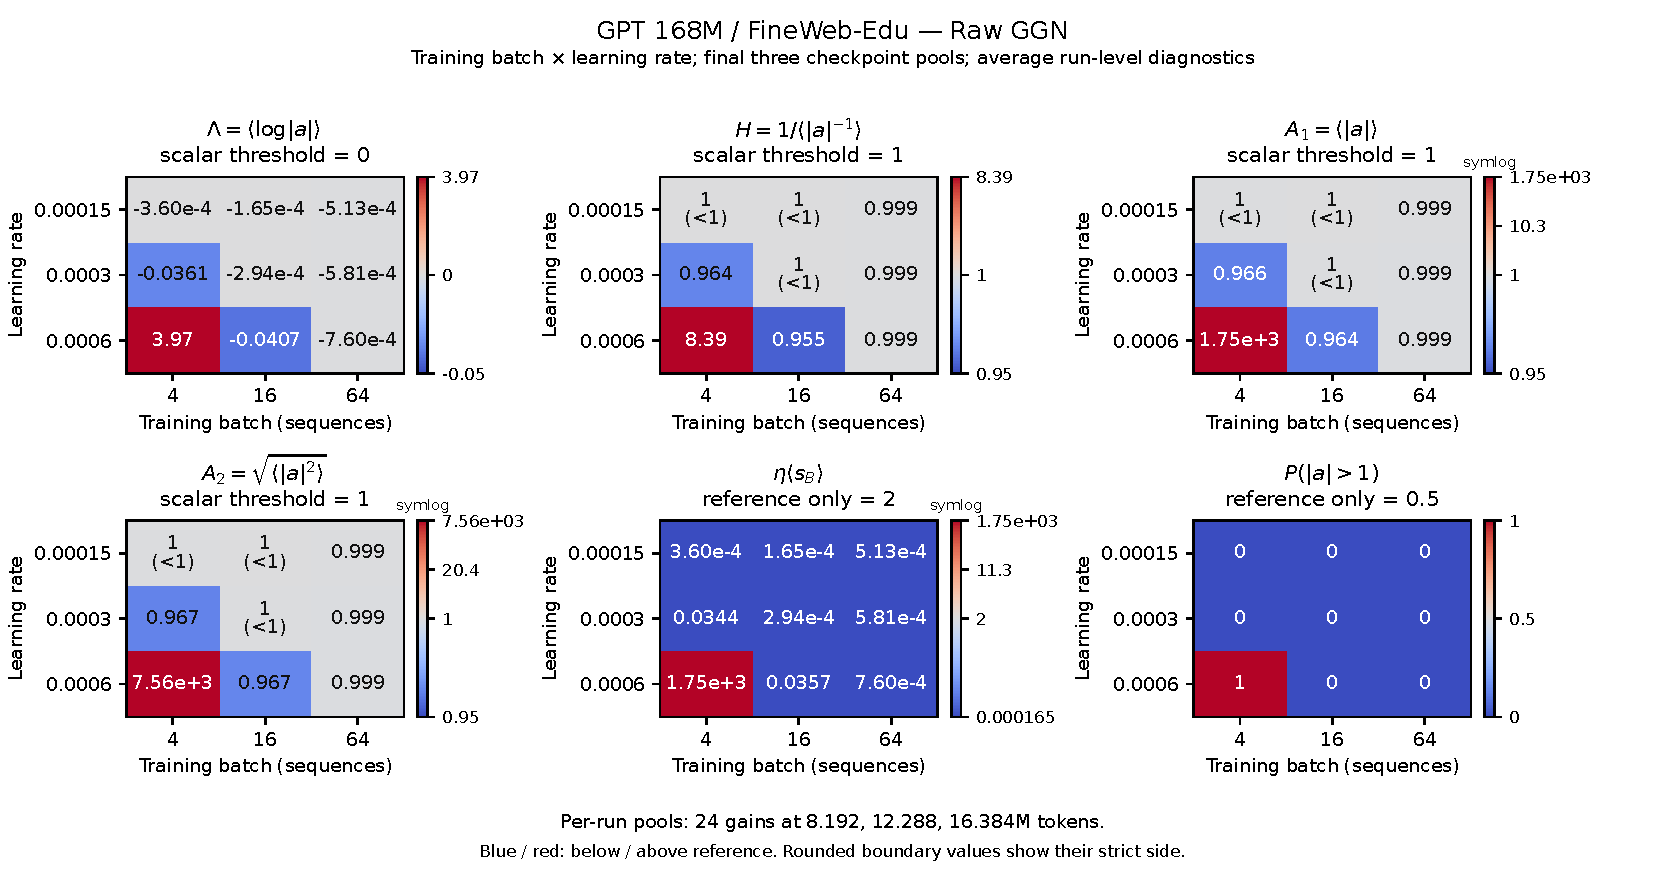
\includegraphics[width=\linewidth,height=0.78\textheight,keepaspectratio]{img/current_results/gpt_grid02_raw_ggn.pdf}
\caption{\textbf{GPT / FineWeb-Edu: batch--step-size grid, raw ggn.} Raw GGN; all nine batch-rate cells retained. Values average run-level statistics from final-three-checkpoint pools at 8.192, 12.288 and 16.384 million tokens. Blue/red means below/above the panel reference. Pools contain 48 Hessian or 24 GGN gains per run. Annotations use three significant figures, with strict inequalities when rounded to a threshold. Symlog colorbars retain extreme values; ticks use original units. Eta E[s\_B]=2 and P(|a|>1)=0.5 are references, not stability certificates. Small inverse-moment samples do not establish population finiteness or stationarity. Parents use Adam: raw metrics are scalar SGD counterfactuals; frozen metrics exclude momentum and preconditioner evolution. Neither is a full-Adam Jacobian.}
\label{fig:current-gpt-grid02-raw-ggn}
\end{figure}\clearpage

\begin{figure}[p]\centering
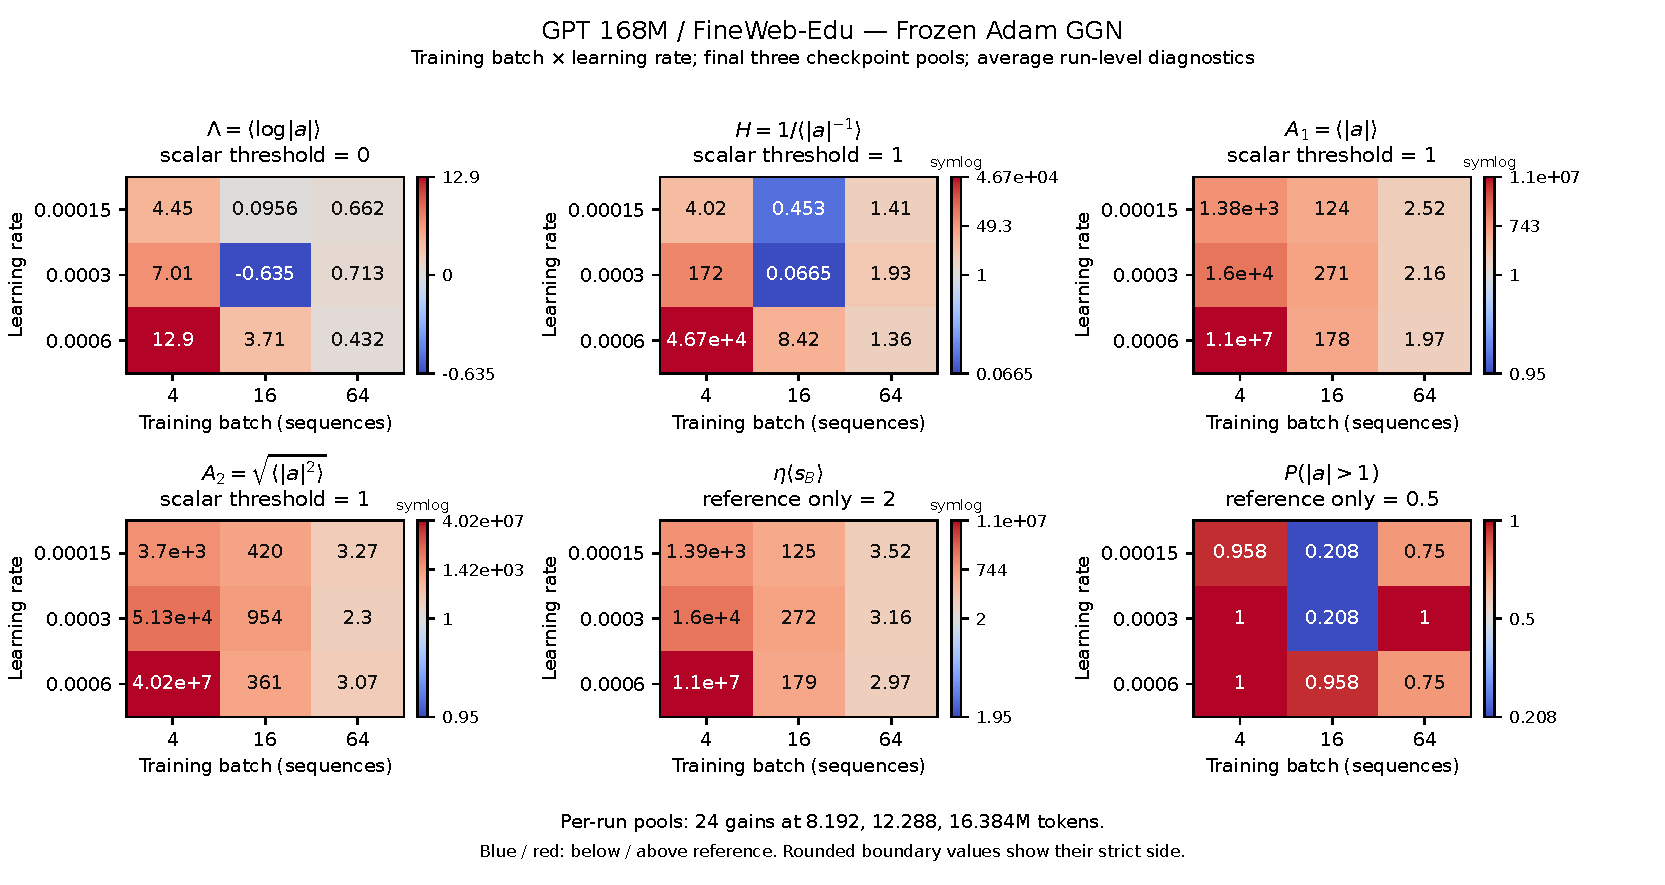
\includegraphics[width=\linewidth,height=0.78\textheight,keepaspectratio]{img/current_results/gpt_grid04_frozen_adam_ggn.pdf}
\caption{\textbf{GPT / FineWeb-Edu: batch--step-size grid, frozen adam ggn.} Frozen Adam GGN; all nine batch-rate cells retained. Values average run-level statistics from final-three-checkpoint pools at 8.192, 12.288 and 16.384 million tokens. Blue/red means below/above the panel reference. Pools contain 48 Hessian or 24 GGN gains per run. Annotations use three significant figures, with strict inequalities when rounded to a threshold. Symlog colorbars retain extreme values; ticks use original units. Eta E[s\_B]=2 and P(|a|>1)=0.5 are references, not stability certificates. Small inverse-moment samples do not establish population finiteness or stationarity. Parents use Adam: raw metrics are scalar SGD counterfactuals; frozen metrics exclude momentum and preconditioner evolution. Neither is a full-Adam Jacobian.}
\label{fig:current-gpt-grid04-frozen-adam-ggn}
\end{figure}\clearpage

\end{document}
